% !TEX program = xelatex
% \documentclass[cn,blue,14pt,screen]{elegantnote}
% pad、pc、kindle、normal、screen
\documentclass[cn,blue,12pt,normal]{elegantnote}
\title{高等数值分析}
\author{\href{mailto:zhangxinhang19@foxmail.com}{张鑫航}}
\institute{国防科技大学}
\version{1.0}
\date{\zhtoday}

\usepackage{array}
\usepackage{bigstrut}
\usepackage{float}
\usepackage{multirow}
\usepackage{wrapfig}
\usepackage{colortbl}
\usepackage{cancel}
\usepackage{amsmath}
%green color
\definecolor{main1}{RGB}{210,168,75}
\definecolor{seco1}{RGB}{9,80,3}
\definecolor{thid1}{RGB}{0,175,152}
%cyan color
\definecolor{main2}{RGB}{239,126,30}
\definecolor{seco2}{RGB}{0,175,152}
\definecolor{thid2}{RGB}{236,74,53}
%cyan color
\definecolor{main3}{RGB}{127,191,51}
\definecolor{seco3}{RGB}{0,145,215}
\definecolor{thid3}{RGB}{180,27,131}

%  ---自定义命令区--- %
% 破折号
\newcommand{\pozhehao}{\kern0.2em\rule[0.8ex]{1.6em}{0.1ex}\kern0.2em}
\newcommand{\xiaopozhe}{\kern0.2em\rule[0.8ex]{0.6em}{0.1ex}\kern0.2em}
% 星号
\usepackage{tikz}
\usepackage{pgfplots}
\usetikzlibrary{shapes.geometric}
\newcommand{\Stars}[2][fill=yellow,draw=orange]{\begin{tikzpicture}[baseline=-0.35em,#1]
\foreach \X in {1,...,5}
{\pgfmathsetmacro{\xfill}{min(1,max(1+#2-\X,0))}
\path (\X*1.1em,0) 
node[star,draw,star point height=0.25em,minimum size=1em,inner sep=0pt,
path picture={\fill (path picture bounding box.south west) 
rectangle  ([xshift=\xfill*1em]path picture bounding box.north west);}]{};
}
\end{tikzpicture}}
% 选择题 \choice{#1}{#2} #1=1选项为答案、#2=[A/B/C/D]为序号
\newcommand{\choice}[2]{
    \if #1==\textcolor{white}{0}
        \colorbox{black!30}{\textcolor{white}{#2}}
    \else
        \colorbox{cyan!50}{\textcolor{white}{#2}}
    \fi
}
% 填空题
\newcommand{\sol}[1]{
    \colorbox{cyan!50}{[#1]}
}
\newcommand{\diff}{\mathrm{d}}
% latexdiff
%DIF PREAMBLE EXTENSION ADDED BY LATEXDIFF
%DIF UNDERLINE PREAMBLE %DIF PREAMBLE
\RequirePackage[normalem]{ulem} %DIF PREAMBLE
\RequirePackage{color}\definecolor{RED}{rgb}{1,0,0}\definecolor{BLUE}{rgb}{0,0,1} %DIF PREAMBLE
\providecommand{\DIFadd}[1]{{\protect\color{blue}\uwave{#1}}} %DIF PREAMBLE
\providecommand{\DIFdel}[1]{{\protect\color{red}\sout{#1}}}                      %DIF PREAMBLE
%DIF SAFE PREAMBLE %DIF PREAMBLE
\providecommand{\DIFaddbegin}{} %DIF PREAMBLE
\providecommand{\DIFaddend}{} %DIF PREAMBLE
\providecommand{\DIFdelbegin}{} %DIF PREAMBLE
\providecommand{\DIFdelend}{} %DIF PREAMBLE
%DIF FLOATSAFE PREAMBLE %DIF PREAMBLE
\providecommand{\DIFaddFL}[1]{\DIFadd{#1}} %DIF PREAMBLE
\providecommand{\DIFdelFL}[1]{\DIFdel{#1}} %DIF PREAMBLE
\providecommand{\DIFaddbeginFL}{} %DIF PREAMBLE
\providecommand{\DIFaddendFL}{} %DIF PREAMBLE
\providecommand{\DIFdelbeginFL}{} %DIF PREAMBLE
\providecommand{\DIFdelendFL}{} %DIF PREAMBLE
%DIF END PREAMBLE EXTENSION ADDED BY LATEXDIFF

% 算法环境
\usepackage[linesnumbered,ruled,vlined]{algorithm2e}
\renewcommand{\algorithmcfname}{算法}
\SetKwInOut{KIN}{输入}
\SetKwInOut{KOUT}{输出}
\renewcommand{\thealgocf}{\thesection.\arabic{algocf}} %<---细节与重点(实现连字符编号)
\DontPrintSemicolon 

\begin{document}
\maketitle
\centerline{
  
\includegraphics[width=0.2\textwidth]{figure/logo.pdf}
}
判断$10\times 3'$

大题$6$

\newpage
\tableofcontents
\newpage

% !TeX program = xelatex*2
% !TeX root = ../elegantnote.tex
\section{绪论}
\subsection{误差的来源和分类}
\begin{definition}[舍入误差]
    由于计算机字长的有限性,对相关数据进行存储表示时便产生舍入误差。
\end{definition}
\begin{definition}[截断误差]
    计算机必须在有限的时间内得到运行结果,于是无穷的运算过程必须截断为有限过程,由此产生截断误差。
\end{definition}
\begin{figure}[htbp]
    \centering
    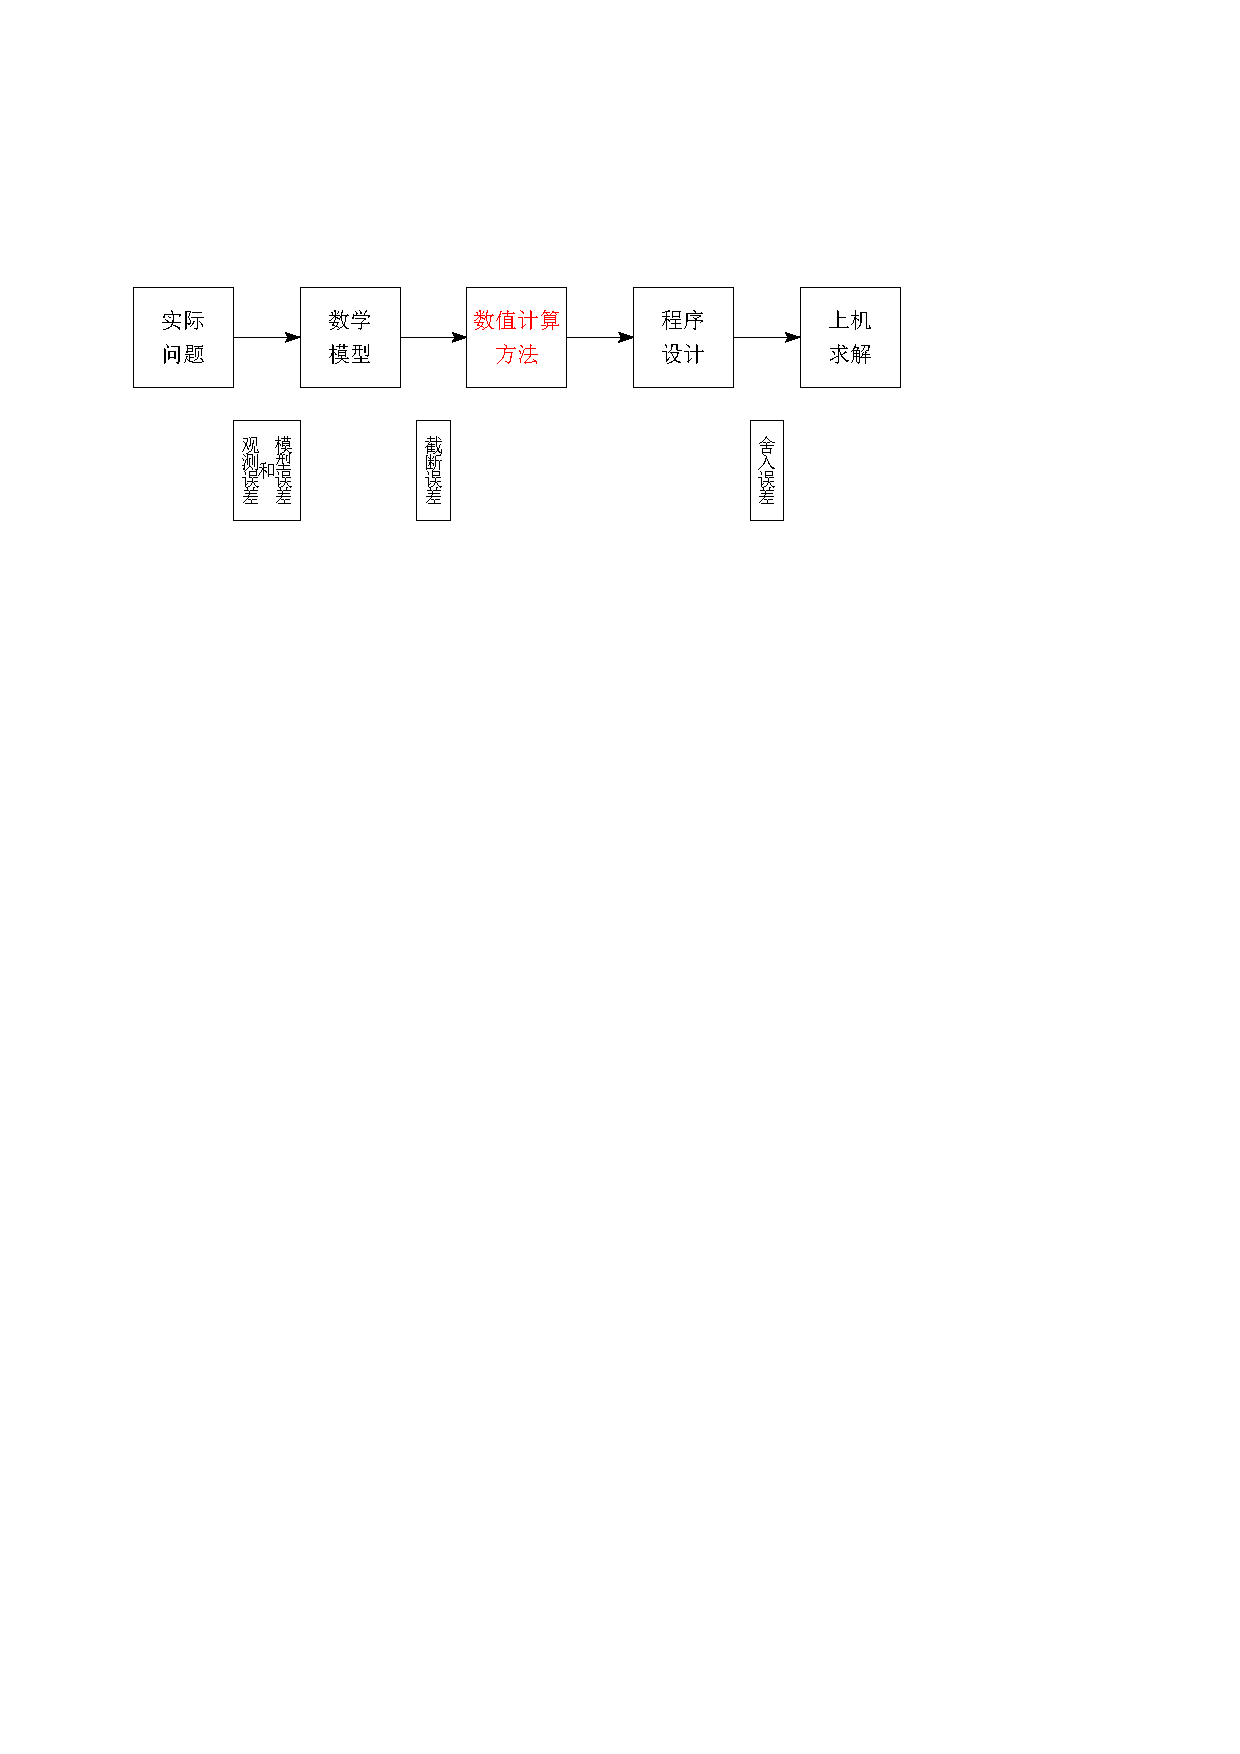
\includegraphics{image/误差.pdf}
\end{figure}
\subsection{误差度量}
\begin{definition}[误差]
    设$x$为精确值(准确值),$x^*$是$x$的一个近似值,称$e^* = x^*-x$为近似$x$的绝对误差或误差。
\end{definition}
\begin{definition}[误差限]
    如果精确值$x$与近似值$x^*$的误差的绝对值不超过某正数$\varepsilon$,即
    \[
        |e| = |x^*-x|<\varepsilon
    \]
    称$\varepsilon$为绝对误差限或误差限。
\end{definition}
\begin{definition}[相对误差]
    设$x$为精确值(准确值),$x^*$是$x$的一个近似值,称$\colorbox{yellow!50}{$r = \dfrac{e^*}{x^*}=\dfrac{x^*-x}{x^*}$}$为近似$x$的相对误差。
\end{definition}
\begin{definition}[相对误差限]
    如果有正数$\varepsilon_r$,使得$r = \left| \dfrac{e^*}{x^*} \right|<\varepsilon_r$,则称$\varepsilon_r$为$x$的相对误差限。
\end{definition}

\begin{definition}[有效数字]
    当$x$的误差限为\colorbox{yellow!50}{某一位}的半个单位,则\colorbox{yellow!50}{这一位}到第一个非零位的位数称为$x$的有效位数。若有效数字共有$n$个,则称$x$有$n$位有效数字,或者说$x$精确到$n$位。
    
    或者说对于用标准形式表示的近似值$x^*$
    \[
        \begin{array}{c}
            x^* = \pm 10^m\times \left( a_1+a_2\times 10^{-1}+\cdots+a_n\times 10^{-(n-1)} \right)\\
            a_{i}\in\left\{ 1,2,\cdots 9 \right\},\,i = 1,2,\cdots n-1
        \end{array}
    \]
    有
    \[
        |x^*-x|< \dfrac{1}{2}\times 10^{m-n+1}
    \]
\end{definition}
\begin{theorem}
    对于用标准形式表示的近似值$x^*$
    \[
        \begin{array}{c}
            x^* = \pm 10^m\times \left( a_1+a_2\times 10^{-1}+\cdots+a_n\times 10^{-(n-1)} \right)\\
            a_{i}\in\left\{ 1,2,\cdots 9 \right\},\,i = 1,2,\cdots n-1
        \end{array}
    \]
    若$x^*$具有$n$位有效数字,则其相对误差限为
    \[
        r\leqslant \dfrac{1}{2a_1}\times 10^{-(n-1)}
    \]
    反之,若$x^*$的相对误差限$r\leqslant \dfrac{1}{2(a_1+1)}\times 10^{-(n-1)}$,则$x^*$至少具有$n$位有效数字。
\end{theorem}
\begin{proof}
    对于$x^*$有
    \[
        a_1\times 10^{m} \leqslant|x^*|\leqslant(a_1+1)\times 10^{m}  
    \]
    则,相对误差限$r$
    \[
        r = \dfrac{|x^*-x|}{|x^*|} \leqslant \dfrac{\dfrac{1}{2}\times 10^{m-n+1}}{a_1\times 10^{m}} = \dfrac{1}{2a_1}\times 10^{-(n-1)}
    \]
    反之,若$r\leqslant \dfrac{1}{2(a_1+1)}\times 10^{-(n-1)}$,有
    \[
        |x^*-x| = r|x^*|<\dfrac{1}{2(a_1+1)}\times 10^{-(n-1)}\times (a_1+1)\times 10^{m} = \dfrac{1}{2}\times 10^{m-n+1}
    \]
    则$x^*$至少具有$n$位有效数字。证毕!
\end{proof}
\begin{theorem}
    四舍五入所得皆为有效数字。
\end{theorem}
\begin{proof}
    若将精确值$x$表示为
    \[
        x = \pm 10^m\times \left( a_1+a_2\times 10^{-1}+\cdots+a_n\times 10^{-(n-1)}+a_{n+1}\times 10^{-n}+\cdots \right)
    \]
    将$x$四舍五入到第$n$位得到$x^*$
    \[
        x^* = \pm 10^m\times \left( a_1+a_2\times 10^{-1}+\cdots+a_n^{\prime}\times 10^{-(n-1)} \right)
    \]
    对于四舍五入到第$n$位得到的$x^*$,有以下两种情况:
    \begin{enumerate}
        \item $a_n^{\prime}-a_n = 0,\ a_{n+1}<5$(靠近原点)
        \[
            \left| (a_n^{\prime}-a_n) - a_{n-1}\times 10^{-1} \right|<\dfrac{1}{2}
        \]
        \item $a_n^{\prime}-a_n = 1,\ 5\leqslant a_{n+1}<10$(远离原点)
        \[
            \left| (a_n^{\prime}-a_n) - a_{n-1}\times 10^{-1} \right|<\dfrac{1}{2}
        \]
    \end{enumerate}
    那么$|x^*-x|$有
    \[
        \begin{array}{ll}
            |x^*-x| &= 10^{m-n+1}\times \left| (a_n-a_n^{\prime}) + a_{n-1}\times 10^{-1} \right|\\
            &<\dfrac{1}{2}\times 10^{m-n+1}
        \end{array} 
    \]证毕!
\end{proof}
\begin{note}
    误差的传播:记$x^*$和$y^*$分别为$x$和$y$的近似值,则初始误差与计算结果中产生的误差有下列关系
    \[
        \varepsilon_{x^*\pm y^*} = \varepsilon_{x^*}+\varepsilon_{y^*},\ \varepsilon_{r_{x^*\pm y^*}} = \dfrac{\varepsilon_{x^*}+\varepsilon_{y^*}}{x^{*}\pm y^{*}}
    \]
    \[
        \varepsilon_{x^*\cdot y^*} = x^*\varepsilon_{y^*}+y^*\varepsilon_{x^*},\ \varepsilon_{r_{x^*\cdot y^*}} = \dfrac{x^*\varepsilon_{y^*}+y^*\varepsilon_{x^*}}{x^{*}\cdot y^{*}}
    \]
    \[
        \varepsilon_{\frac{x^*}{y^*}} \approx \dfrac{x^*\varepsilon_{y^*}+y^*\varepsilon_{x^*}}{y^{*2}},\ \varepsilon_{r_{\frac{x^*}{y^*}}} \approx \dfrac{x^*\varepsilon_{y^*}+y^*\varepsilon_{x^*}}{x^{*}\cdot y^{*}}
    \]
    \[
        \begin{array}{c}
            \varepsilon(f(\boldsymbol{x}^*))\approx \sum\limits_{i = 1}^{n}\left|\dfrac{\partial f(\boldsymbol{x}^*)}{\partial x_i}\right|\varepsilon(x_i^*)\\
            \varepsilon_r(f(\boldsymbol{x}^*))\approx \sum\limits_{i = 1}^{n}\left|\dfrac{\partial f(\boldsymbol{x}^*)}{\partial x_i}\right|\dfrac{\varepsilon(x_i^*)}{f(\boldsymbol{x}^*)}
        \end{array}
    \]
\end{note}
\begin{example}
    设$V = \dfrac{4\pi R^3}{3}$,当半径$R$有误差时,求球体积$V$的相对误差与$R$的相对误差的关系。\Stars{3.5}{}
    \[
        e_r[V] = \dfrac{e[V]}{V} = \dfrac{4\pi R^2\cdot e[R]}{\dfrac{4\pi R^3}{3}} = 3\dfrac{e[R]}{R} = 3e_r{R}
    \]
\end{example}
\begin{example}
    设$x>0$,$x$的相对误差为$\delta$,求$\ln x$的误差。\Stars{4}{}
    \[
        \ln x-\ln x^* = \ln \dfrac{x}{x^*} = \ln \dfrac{x-x^*+x^*}{x^*} = \ln (\delta+1)\approx \delta
    \]
    或者
    \[
        e(\ln x^*) \approx \dfrac{e(x^*)}{x^*} = e_r(x^*) = \delta
    \]
\end{example}
\begin{example}
    设$x$的相对误差为$2\%$,求$x^n$的相对误差。\Stars{4}{}
    \[
        e_r(x^n)\approx n\dfrac{x^{*(n-1)}e(x^*)}{x^{*(n)}} = ne_r(x^*) = 0.02n
    \]
\end{example}

\subsection{误差分析方法与原则}
\begin{definition}[病态问题]
    对于一个数值问题,若输入数据的微小扰动(即误差)会引起输出数据(即问题解)相对误差很大,这就是\textcolor{red!50}{病态问题}。
\end{definition}
\begin{definition}[数值稳定性]
    一个算法如果原始数据有扰动(即误差),二计算过程中舍入误差不增长,则称此算法是数值稳定的;否则,若误差增长则称算法数值不稳定。
\end{definition}
\begin{note}
    数值运算中误差分析的方法与原则
    \begin{itemize}
        \item 避免除数的绝对值远远小于被除数
        \item 避免两相近数相减
        \item 防止大数“吃掉”小数
        \item 注意简化计算步骤,减少运算次数
    \end{itemize}
\end{note}
% !TeX program = xelatex*2
% !TeX root = ../elegantnote.tex
\section{数值逼近}
\subsection{插值法}
\begin{definition}[插值函数]
    已知函数$y = f(x)$在互异节点$\left\{ x_i \right\}_{i = 0}^{n}\subset \left[ a,b \right]$处的函数值$\left\{ y_i = f(x_i) \right\}_{i = 0}^{n}$,若存在简单函数$p(x)$,使得
    \begin{equation}\label{eq:chazhi}
        p(x_i) = y_i,\ (i = 0,1,\dots,n)
    \end{equation}
    成立,则称$p(x)$是$f(x)$关于节点$\left\{ x_i \right\}_{i = 0}^{n}$的一个插值函数。
    $\left\{ x_i \right\}_{i = 0}^{n}$——插值节点,$\left[ a,b \right]$——插值区间,$f(x)$——被插值函数。
\end{definition}
\begin{note}
    用$p(z)$的值作为$f(z)$的近似值,当元在节点形成的区间上时,称该方法为内插法﹔当元不在节点形成的区间上但在插值区间上,则称该方法为外插法。
\end{note}
\begin{note}
    当插值函数$p(z)$为多项式时,称 $p(x)$是$f(x)$的一个插值多项式。插值余项$R(x)\overset{\text{def}}{=}f(x)-p(x)$,插值余项又称为截断误差。
\end{note}
\begin{theorem}[插值多项式的存在惟一性定理]
    满足插值条件(\ref{eq:chazhi})的不超过$n$次的插值多项式$p(x)$是存在唯一的。
\end{theorem}
\begin{corollary}
    若$f(\alpha)$是不超过$n$次的多项式,则它的关于$n+1$个互异节点$\left\{ x_i \right\}_{i = 0}^{n}$的不超过$n$次的插值多项式$p(x)$与被插值函数$f(x)$恒等,即有
    \[
        p(x)\equiv f(x)
    \]
\end{corollary}
\begin{note}
    误差的估计:
    \begin{itemize}
        \item 若被插值函数$f(x)\in \boldsymbol{C}^{n+1}\left[ a,b \right]$,则有插值误差估计式
        \[
            \left| R_{n}(x) \right|\leqslant \dfrac{M_{n+1}}{(n+1)!}\left| \omega_{n+1}(x) \right|
        \]
        \item 若仅需估计某一点$\bar{x}^*$处的插值误差,则利用
        \[
            \left| R(\bar{x}) \right|\leqslant \dfrac{M_{n+1}}{(n+1)!}\left| \omega_{n+1}(\bar{x}) \right|,\,\bar{x} \in \left[ a,b \right]
        \]
        \item 若要估计在整个插值区间上的误差,用
        \[
            \left| R(\bar{x}) \right|\leqslant \dfrac{M_{n+1}}{(n+1)!}\left| \omega_{n+1}(x) \right|,\,\forall x \in \left[ a,b \right]
        \]
        其中,$M_{n+1}$和$\max\limits_{x\in [a,b]} |\omega_{n+1}(x)|$用微积分中求极值的方法进行。
    \end{itemize}
\end{note}
\subsection{Lagrange插值}
设$p(x)$是形如$p(x) = a_0+a_1x+a_2x^2+\cdots+a_nx^n$,根据$n+1$个互异节点$\left\{ x_i \right\}_{i = 0}^{n}$,得到
\[
    \begin{cases}a_0+a_1x_0+\cdots+a_nx_0^n=y_0,\\a_0+a_1x_1+\cdots+a_nx_1^n=y_1,\\\vdots\\a_0+a_1x_n+\cdots+a_nx_n^n=y_n.\end{cases}
\]
因为
\[
    V_n(x_0,x_1,\cdots,x_n)=\left.\left|\begin{array}{ccccc}1&x_0&x_0^2&\cdots&x_0^n\\1&x_1&x_1^2&\cdots&x_1^n\\\vdots&\vdots&\vdots&&\vdots\\1&x_n&x_n^2&\cdots&x_n^n\end{array}\right.\right|\neq 0
\]
所以方程存在唯一一组解$a_0,a_1,\cdots,a_n$,故而拉格朗日插值多项式也存在且唯一。
\[
    p_n(x) = L_n(x) = \sum\limits_{i = 0}^{n}f(x_i)l_i(x)
\]
拉格朗日插值多项式需要满足$p_{n}(x_i) = f(x_i)$,故而$n$次多项式$l_i(x)$需要满足
\[
    l_i(x_j) = \left\{
        \begin{array}{ll}
            1, & j = i\\
            0, & j\neq i
        \end{array}
    \right.
\]
可以将拉格朗日插值基函数$\left\{ l_i(x) \right\}_{i = 0}^{n}$的定义如下:
\[
    l_{i}(x) = \prod\limits_{\substack{j = 0\\ j\neq i}}\dfrac{x-x_j}{x_i-x_j} = \dfrac{\omega_{n+1}(x)}{(x-x_i)\omega_{n+1}'(x_i)}
\]
其中
\[
    \begin{array}{l}

        \omega_{n+1}(x) = (x-x_0)(x-x_1)\cdots(x-x_n)\\
        \omega'_{n+1}(x_k) = (x_k-x_0)\cdots(x_k-x_{k-1})(x_k-x_{k+1})(x_k-x_n)\\
    \end{array}
\]
\begin{theorem}[插值余项定理]
    设$f^{n}(x)$在$\left[ a,b \right]$上连续,$f^{n+1}(x)$在$\left( a,b \right)$上存在,节点$a\leqslant x_0<x_1<\cdots<x_n\leqslant b$,$L_{n}(x)$是满足条件$p_{n}(x_i) = f(x_i)$的多项式,则对任何$x\in\left[ a,b \right]$,插值余项
    \[
        R_n(x) = f(x)-L_n(x) = \dfrac{f^{(n+1)}(\xi)}{(n+1)!}\omega_{n+1}(x)
    \]
    这里,$\xi\in(a,b)$且依赖于$x$。
\end{theorem}
\begin{proof}
    由给定条件知,$R_n(x)$在$\left\{ x_i \right\}_{i = 0}^{n}$上为0,即
    \[
        R_n(x_i) = 0
    \]
    于是
    \[
        R_n(x) = K(x)\omega_{n+1}(x)
    \]
    其中$K(x)$是与$x$有关的待定系数。
    现在把$x$看成$\left[ a,b \right]$上的一个固定点,做函数
    \[
        \phi(t) = f(t)-L_n(t)-K(x)\omega_{n+1}(t)
    \]
    容易知道$\phi(t)$在点$x,x_0,\cdots,x_n$这$n+2$个点上满足$\phi(t) = 0$,反复利用Rolle定理,知道
    \[
        \phi^{(n+1)}(\xi) = f^{(n+1)}(\xi)-(n+1)!K(x) = 0
    \]
    于是
    \[
        K(x) = \dfrac{f^{(n+1)(\xi)}}{(n+1)!}
    \]
    证毕!
\end{proof}
\begin{remark}
    $\xi$在$(a,b)$内的具体位置通常不可能给出,如果可以求出$\max\limits_{a\leqslant x\leqslant b}|f^{(n+1)}(x)| = M_{n+1}$,那么插值多项式$L_n(x)$逼近$f(x)$的截断误差是
    \[
        |R_n(x)|\leqslant \dfrac{M_{n+1}}{(n+1)!}|\omega_{n+1}(x)|
    \]
\end{remark}
\begin{corollary}
    若$f(x)$是不超过$n$次的多项式,则它的关于$n+1$个互异节点$\left\{ x_i \right\}_{i = 0}^{n}$$n$次的拉格朗日插值多项式$L_{n}(x)$有
    \[
        R_{n}(x) = f(x)-L_{n}(x) = 0
    \]
    即
    \[
        f(x) = L_{n}(x) = \sum\limits_{i = 0}^{n}f(x_i)l_{i}(x)
    \]
\end{corollary}
\begin{example}
    证明$\sum\limits_{i = 0}^{5}\left( x-x_i \right)^2l_{i}(x) = 0$,其中$l_{i}(x)$是关于$\left\{ x_0,x_1,\cdots, x_5 \right\}$的插值基函数。\Stars{5}
    \begin{proof}
        \[
            \begin{array}{ll}
                \sum\limits_{i = 0}^{5}\left( x-x_i \right)^2l_{i}(x) & = x^2\sum\limits_{i = 0}^{5}1\cdot l_{i}(x)-2x\sum\limits_{i = 0}^{5}x_i\cdot l_{i}(x)+\sum\limits_{i = 0}^{5}x_{i}^2\cdot l_{i}(x)\\
                &=x^2-2x\cdot x+x^2 = 0
            \end{array}
        \]
        证毕!
    \end{proof}    
\end{example}
\begin{example}
    对一条直线采样10个点进行Lagrange插值,所得插值多项式是\sol{1}次的。
\end{example}
\begin{note}
    Aitken逐次线性插值法:

    用Lagrange插值多项式$L_{n}(x)$计算函数近似值时,如需增加插值节点,那么原来算出来的数据均不能利用,必须重新计算。为克服这个缺点通常可用逐次线性插值方法得到高次插值。

    两个$k$次插值多项式可通过线性插值得到$k+1$次插值多项式
    \begin{equation}\label{eq:Aitken}
        I_{0,1,\cdots,k,l}(x) = I_{0,1,\cdots,k}(x)+\dfrac{I_{0,1,\cdots,k-1,l}(x)-I_{0,1,\cdots,k}(x)}{x_l-x_k}\left( x-x_k \right)
    \end{equation}
    这是关于节点$\left\{ x_0,\cdots,x_{k},x_{l} \right\}$的插值多项式。显然
    \begin{itemize}
        \item 对于$i = 0,1,\cdots,k-1$
        \[
            I_{0,1,\cdots,k,l}(x_i) = I_{0,1,\cdots,k}(x_i) = f(x_i)
        \]
        \item 对于$x_k$
        \[
            I_{0,1,\cdots,k,l}(x_k) = I_{0,1,\cdots,k}(x_k) = f(x_k)
        \]
        \item 对于$x_l$
        \[
            I_{0,1,\cdots,k,l}(x_l) = I_{0,1,\cdots,k}(x_l)+\dfrac{f(x_l)-I_{0,1,\cdots,k}(x_l)}{x_l-x_k}(x_l-x_k) = f(x_l)
        \]
    \end{itemize}
    这证明了(\ref{eq:Aitken})满足插值条件。

    当$k = 0$时为线性插值,当$k = 1$时插值节点为$x_0,x_1,x_l$,插值多项式为
    \[
        I_{0,1,l}(x) = I_{0,1}(x)+\dfrac{I_{0,l}(x)-I_{0,1}(x)}{x_l-x_1}(x-x_1)
    \]
    % Table generated by Excel2LaTeX from sheet 'Aitken逐次线性插值'
    \begin{table}[htbp]
        \centering
        \begin{tabular}{|c|c|c|c|c|c|c|}
            \hline
            $x_0$ & $f(x_0)$ &     &     &     &     & $x-x_0$ \bigstrut\\
            \hline
            $x_1$ & $f(x_1)$ & $I_{0,1}$ &     &     &     & $x-x_1$ \bigstrut\\
            \hline
            $x_2$ & $f(x_2)$ & $I_{0,2}$ & $I_{0,1,2}$ &     &     & $x-x_2$ \bigstrut\\
            \hline
            $x_3$ & $f(x_3)$ & $I_{0,3}$ & $I_{0,1,3}$ & $I_{0,1,2,3}$ &     & $x-x_3$ \bigstrut\\
            \hline
            $x_4$ & $f(x_4)$ & $I_{0,4}$ & $I_{0,1,4}$ & $I_{0,1,2,4}$ & $I_{0,1,2,3,4}$ & $x-x_4$ \bigstrut\\
            \hline
        \end{tabular}%
  \end{table}%
\end{note}
\subsection{Newton插值}
\[
    p_{n}(x) = N_{n}(x) = \sum\limits_{i = 0}^{n}f\left[ x_0,x_1,\cdots,x_i \right]\omega_{i}(x)
\]
其中零阶插商
\[
    f\left[ x_0 \right] = f(x_0),\,\omega_0(x)\equiv 1,\,\omega_{i}(x) = \prod\limits_{k = 0}^{i-1}(x-x_k)
\]
\begin{definition}[差商]
    称$f\left[ x_0,x_k \right]=\dfrac{f(x_k)-f(x_0)}{x_k-x_0}$为函数$f(x)$关于$x_0,x_k$的一阶差商,称
    \[
        f\left[ x_0,x_l,x_k \right] = \dfrac{f\left[ x_0,x_k \right]-f\left[ x_0,x_l \right]}{x_k-x_l}
    \]
    为$f(x)$关于$x_0,x_k,x_l$的二阶差商。一般的称
    \[
        f[x_0,x_1,\cdots,x_m]=\frac{f[x_0,x_1,\cdots,x_{k-2},x_m]-f[x_0,x_1,\cdots,x_{k-2},
        x_{k-1}]}{x_m-x_{k-1}}
    \]
    为$f(x)$的$k$阶差商。
\end{definition}
\begin{note}
    插值误差:把$x$当作$[a,b]$一点,可得
    \[
        \begin{array}{c}
            f(x) = f(x_0)+f\left[ x,x_0 \right](x-x_0)\\
            f(x) = f(x_0)+f\left[ x_0,x_1 \right](x-x_0)+f\left[ x,x_0,x_1 \right](x-x_0)(x-x_1)\\
            \cdots\\
            \begin{array}{ll}
                f(x) &= f(x_0)+f\left[ x_0,x_1 \right](x-x_0)\\
                &+f\left[x_0,x_1,x_2 \right](x-x_0)(x-x_1)+\cdots\\
                &+f\left[ x_0,\cdots,x_n \right](x-x_0)\cdots(x-x_{n-1})\\
                &+f\left[ x,x_0,\cdots,x_n \right]\prod\limits_{i = 0}^{n}(x-x_i)\to\textcolor{red}{\text{插值误差\ or\ }\text{余项}R_{n}(x)}
            \end{array}
        \end{array}  
    \]
    由上,得
    \[
        \begin{array}{c}
            f(x) = N_n(x)+f\left[ x,x_0,\cdots,x_n \right]\prod\limits_{i = 0}^{n}(x-x_i)\\
            \text{和拉格朗日插值对比}\\
            f(x) = L_{n}(x)+\dfrac{f^{(n+1)}(\xi)}{(n+1)!}\omega_{n+1}(x)
        \end{array}
    \]
\end{note}



\begin{note}
    差商有如下性质:
    \begin{enumerate}
        \item $k$阶差商可表示为函数值$f(x_{0}),\cdots,f(x_k)$的线性组合,即
        \[
            f[x_0,x_1,\cdots,x_k]=\sum\limits_{j=0}^k\frac{f(x_j)}{(x_j-x_0)\cdotp\cdotp\cdotp(x_j-x_{j+1})(x_j-x_{j+1})\cdotp\cdotp\cdotp(x_j-x_k)}.
        \]
        这个性质也表明差商与节点的排列顺序无关(插值的对称性)。
        \item 差商与导数的关系
        \begin{equation}\label{eq:MinusQution}
            f[x_0,x_1,\cdots,x_n]=\frac{f^{(n)}(\xi)}{n!},\quad\xi\in[a,b].
        \end{equation}
        \begin{proof}
            \[
                f(x) = N_{n-1}(x)+f\left[ x,x_0,\cdots,x_{n-1} \right]\omega_{n}(x)
            \]
            记$R(x) = f(x)-N_{n-1}(x) = f\left[ x,x_0,\cdots,x_{n-1} \right]\omega_{n}(x)$,固定$x$,令
            \[
                g(t) = f(t)-N_{n-1}(x)-f\left[ x,x_0,\cdots,x_{n-1} \right]\omega_{n}(t)
            \]
            对于$\left\{ x,x_0,\cdots,x_{n-1} \right\}$有
            \[
                g(x) = g(x_0) = \cdots = g(x_{n-1}) = 0    
            \]
            反复利用Rolle定理,得到
            \[
                g^{(n)}(\xi) = f^{(n)}(\xi)-f\left[ x,x_0,\cdots,x_{n-1} \right]n! = 0
            \]
            即(这一步将$x_n$带入$x$,并利用插值的对称性)
            \[
                f[x_0,x_1,\cdots,x_n]=\frac{f^{(n)}(\xi)}{n!},\quad\xi\in[a,b].
            \]
            证毕!
        \end{proof}
    \end{enumerate}
\end{note}
\begin{figure}[htbp]
    \centering
    
\includegraphics{image/Newton插值表.pdf}
\end{figure}
\subsubsection{差分与等距节点插值公式}
设等式$y = f(x)$在等距节点$x_k = x_0+kh\,(k = 0,1,\cdots,n)$上的值$f_k = f(x_k)$为已知,这里$h$为常数,称为步长。
\begin{definition}[偏差]
    \[
        \begin{array}{c}
            \Delta f_k = f_{k+1}-f_k\\
            \nabla f_k = f_{k}-f_{k-1}\\
            \delta f_k=f(x_k+h/2)-f(x_k-h/2)=f_{k+\frac12}-f_{k-\frac12}
        \end{array}
    \]
    分别为向前差分、向后差分以及中心差分。
\end{definition}
\begin{corollary}[差商与差分的关系\Stars{5}]
    \[
        f\left[ x_k,x_{k+1},\cdots,x_{k+m} \right] = \dfrac{1}{m!}\dfrac{1}{h^m}\Delta^mf_{k},\,(m = 1,2,\cdots,n)
    \]
    \[
        f\left[ x_k,x_{k-1},\cdots,x_{k-m} \right] = \dfrac{1}{m!}\dfrac{1}{h^m}\Delta^mf_{k}
    \]
    同时利用(\ref{eq:MinusQution})可以得到
    \[
        \Delta^nf_{k} = h^nf^{(n)}(\xi),\,\xi\in(x_k,x_{k+n})
    \]
\end{corollary}

\subsection{Hermite插值}
不少实际问题不但要求在节点上函数值相等,而且还要求它的导数值相等,甚至要求高阶导数值也相等.满足这种要求的插值多项式就是Hermite插值多项式.

已知节点$\left\{ x_{j} \right\}_{j = 0}^{n}$,满足
\[
    H(x_j) = y_{j},\,H^{\prime}(x_{j}) = m_{j} = f^{\prime}(x_{j})
\]
可以确定$2n+1$次的多项式
\begin{equation}\label{eq:2n+1Hermite}
    H_{2n+1}(x) = a_0+a_1x+\cdots+a_{2n+1}x^{2n+1}
\end{equation}
插值误差
\[
    R_{n}(x)  =\dfrac{f^{(2n+2)}(\xi)}{(2n+2)!}\omega_{n+1}^2(x)
\]
用基函数表示(\ref{eq:2n+1Hermite})为
\[
    H_{2n+1}(x) = \sum\limits_{i = 0}^{n}\left[ \alpha_{i}(x)f_{i}+\beta_{i}(x)f'_{i} \right]
\]
其中$\alpha_{i}(x)$和$\beta_{i}(x)$均为$2n+1$次多项式,且满足
\begin{equation}\label{eq:constrainHermit}
    \left\{
        \begin{array}{ll}
            \alpha_{i}(x_k) = \delta_{ik}, & \alpha_{i}^{\prime}(x_k) = 0\\
            \beta_{i}(x_k) = 0, & \beta_{i}^{\prime}(x_k) = \delta_{ik}\\
        \end{array}
    \right.
\end{equation}
\begin{note}
    下面的问题就是求满足条件(\ref{eq:constrainHermit})的基函数$\alpha_{i}$和$\beta_{i}(x)$。
    \begin{itemize}
        \item 先求$\alpha_{i}(x)$,可利用Lagrange插值基函数$l_{i}(x)$,令(1.$2n+1$次多项式,2.在$x_j \neq x_i$处为2重零点)
        \[
            \alpha_{i}(x) = [a(x-x_i)+b]l_{i}^2(x)
        \]
        其中$l_{i}(x) = \prod\limits_{j = 0,j\neq i}^{n}\dfrac{x-x_j}{x_i-x_j}$。由$\alpha_{i}(x_i) = 1$,知$b = 1$;由$\alpha_{i}^{\prime}(x_i) = 0$知
        \[
            \begin{array}{l}
                al_{i}^2(\colorbox{cyan!50}{$x_i$})+2[a(\colorbox{cyan!50}{$x_i$}-x_i)+1]l_{i}(\colorbox{cyan!50}{$x_i$})l_{i}^{\prime}(\colorbox{cyan!50}{$x_i$}) = 0\\
                a = -2l_{i}^{\prime}(x_i)\\
                \left( \ln l_{i}(x_i) \right)' = \dfrac{l_{i}^{\prime}(x_i)}{l_{i}(\colorbox{cyan!50}{$x_i$})} = \sum\limits_{\substack{j = 0\\j\neq i}}^{n}\dfrac{1}{(x_i-x_j)}\\
                a = -2\sum\limits_{\substack{j = 0\\j\neq i}}^{n}\dfrac{1}{(x_i-x_j)}\\
            \end{array}
        \]
        故而有
        \[
            \alpha_{i}(x) = \left[1-2(x-x_i)\sum\limits_{\substack{j = 0\\j\neq i}}^{n}\dfrac{1}{(x_i-x_j)}\right]l_{i}^2(x)
        \]
        \item 再求$\beta_{i}(x)$,同理设$\beta_{i}(x) = [a(x-x_i)+b]l_{i}^2(x)$(1.$2n+1$次多项式,2.在$x_j \neq x_i$处为2重零点)。由$\beta_{i}(x_i) = 0$,知$b = 0$;由$\beta_{i}^{\prime}(x_i) = 1$知,
        \[
            \begin{array}{l}
                al_{i}^2(\colorbox{cyan!50}{$x_i$})+2[a(\colorbox{cyan!50}{$x_i$}-x_i)+0]l_{i}(\colorbox{cyan!50}{$x_i$})l_{i}^{\prime}(\colorbox{cyan!50}{$x_i$}) = 1\\
                a = 1
            \end{array}
        \]
        故而有
        \[
            \beta_{i}(x) = (x-x_i)l_{i}^2(x)
        \]
    \end{itemize}
    综上,
    \[
        \begin{array}{l}
            \alpha_{i}(x) = \left[1-2(x-x_i)\sum\limits_{j = 0,j\neq i}^{n}\dfrac{1}{(x_i-x_j)}\right]l_{i}^2(x)\\
            \beta_{i}(x) = (x-x_i)l_{i}^2(x)
        \end{array}
    \]
\end{note}
\begin{example}
    设$f(x) = \ln x$,给定$f(1) = 0,f(2) = 0.693147,f'(1) = 1,f'(2) = 0.5$,用三次Hermite插值多项式$H_3(x)$计算$f(1.5)$的近似值。\Stars{5}{}
    
    请写出$x = 1$处的导数值基函数$\beta_1(x)$和$x = 2$处的函数值基函数$\alpha_2(x)$
    \begin{solution}
        $\beta_{1}(x) = (x-1)\left[ \dfrac{(x-2)}{1-2} \right]^2,\quad \alpha_2(x) = \left[ 1-2(x-2)\dfrac{1}{2-1} \right]\left[ \dfrac{(x-1)}{2-1} \right]^2$
    \end{solution}
\end{example}
\begin{example}
    求一个次数不高于四次的多项式$p(x)$,使它满足$p(0) = p'(0) = 0,\,p(1) = p'(1) = 1,\,p(2) = 1$。\Stars{5}{}
    \begin{solution}
        [解法一]:
        设$p(x) = \left[ \alpha_1(x)p(0)+\alpha_2(x)p(1)+\alpha_3(x)p(2) + \beta_1(x)p'(0)+\beta_2(x)p'(1) \right]$,满足
        % Table generated by Excel2LaTeX from sheet 'Hermit插值'
        \begin{table}[htbp]
            \centering
            \begin{tabular}{|c|c|c|c|c|c|}
            \hline
                & \multicolumn{3}{c|}{函数值} & \multicolumn{2}{c|}{导数值} \bigstrut\\
            \hline
                & 0   & 1   & 2   & 0   & 1 \bigstrut\\
            \hline
            $\alpha_1(x)$ & 1   & 0   & 0   & 0   & 0 \bigstrut\\
            \hline
            $\alpha_2(x)$ & 0   & 1   & 0   & 0   & 0 \bigstrut\\
            \hline
            $\alpha_3(x)$ & 0   & 0   & 1   & 0   & 0 \bigstrut\\
            \hline
            $\beta_1(x)$ & 0   & 0   & 0   & 1   & 0 \bigstrut\\
            \hline
            $\beta_2(x)$ & 0   & 0   & 0   & 0   & 1 \bigstrut\\
            \hline
            \end{tabular}%
        \end{table}%
        可以设
        \[
            \begin{array}{l}
                \alpha_{1}(x) = (ax+b)(x-1)^2(x-2) \\
                \alpha_{2}(x) = (ax+b)x^2(x-2) \\
                \alpha_{3}(x) = bx^2(x-1)^2 \\ 
                \beta_{1}(x) = (ax+b)x(x-1)^2 \\
                \beta_{2}(x) = (ax+b)x^2(x-1)
            \end{array}    
        \]
        上述做法要解多个2元方程,虽然每个方程计算量不大。

        [解法二]:可以看出关于$x = 0$为二重根,设$p(x) = (ax^2+bx+c)x^2$,可以通过求解1个三元方程组

        [解法三]:由给定的条件,可确定次数不超过4的插值多项式
        \[
            p(x) = f(0) + f[0,1](x-0) + f[0,1,2](x-0)(x-1) + (ax+b)(x-0)(x-1)(x-2)
        \]
    \end{solution}
\end{example}

\begin{example}
    求次数不高于三次的多项式$p(x)$,使得$p(x_i) = f(x_i)(i = 0,1,2)$及$p'(x_1) = f'(x_1)$的插值多项式\Stars{4}{}
    
    \begin{solution}
        可以设$p(x)$为
        \[
            \begin{array}{l}
                p(x) = f(x_0) + f[x_0,x_1](x-x_0) + f[x_0,x_1,x_2](x-x_0)(x-x_1) + \\
                A(x-x_0)(x-x_1)(x-x_2)
            \end{array}
        \]
        可以得到
        \[
            A = \dfrac{f'(x_1)-f[x_0,x_1]-f[x_0,x_1,x_2](x_1-x_0)}{(x_1-x_0)(x_1-x_2)}
        \]
    \end{solution}
\end{example}

\subsection{分段低次插值}
\subsubsection{分段线性插值}
设已知节点$a=x_0<x_1<\cdots<x_n=b$上的函数值为$f_0,f_{1}, \cdots , f_{n}, h_{i}= x_{i+ 1}- x_{i}$, $h= \max _{0\leq i\leq n- 1}h_{i}$,若一折线$I_h(x)$满足条件:
\begin{enumerate}
    \item $I_{h}(x)\in C[a,b];$
    \item $I_{h}(x_{i})=f_{i},i=0,1,\cdots,n;$
    \item $I_{h}(x)$在每个小区间$[x_i,x_{i+1}](i=0,1,\cdots,n-1)$上为线性函数。
\end{enumerate}
则称$I_h(x)$为分段线性函数,相应的插值为分段线性插值。
\[
    I_h(x)=\frac{x-x_{i+1}}{x_i-x_{i+1}}f_i+\frac{x-x_i}{x_{i+1}-x_i}f_{i+1},\quad x\in[x_i,x_{i+1}]
\]
\begin{example}
    分段线性插值可否用基函数表示,若能,请写出基函数;若不能,请说明理由
    \begin{solution}
        其基函数可表示为
        \[
            l_{i}(x) = \left\{
                \begin{aligned}
                    \frac{x-x_{i-1}}{x_{i}-x_{i-1}}, & x_{i-1}\leq x \leq x_{i}\\
                    \frac{x-x_{i+1}}{x_{i}-x_{i+1}}, & x_{i}\leq x \leq x_{i+1}\\
                    0, & \text{其他}
                \end{aligned}
            \right.
        \]
    \end{solution}
\end{example}
\begin{note}
    分段线性插值的误差估计
    \begin{itemize}
        \item 若$f(x)\in C[a,b]$,则当$h\to0$时$I_h(x)$一致收敛于$f(x)$。
        \item 若$f(x)\in C^{2}[a,b]$,则余项$R(x)=f(x)-I_{h}(x)$有估计式
        \[
            \mid R(x)\mid\leq\frac{Mh^2}{8},M=\max_{a\leq x\leq b}\mid f''(x)\mid 
        \]
    \end{itemize}
\end{note}
\subsubsection{分段Hermite插值}
\begin{definition}[分段Hermite插值]
    设已知节点$a = x_0<x_1<\cdots <x_n<b$上的函数值为$f_0,f_1,\cdots,f_n$,导数值为$f_0',f_1',\cdots,f_n'$满足插值条件
    \begin{itemize}
        \item $I_{h}(x)\in C^1\left[ a,b \right]$
        \item $I_{h}(x_i) = f_i,\,I_{h}'(x_i) =f_{i}'$
        \item $I_{h}(x)$在每个小区间为3次多项式
    \end{itemize}
\end{definition}

\subsection{三次样条插值}
\begin{definition}[三次样条插值]
    给定$[a,b]$上$n+1$个节点$a = x_0<x_1<\cdots<x_n = b$和这些点上的函数值$f(x)_i = y_i,\,i = 0,1,\cdots,n$。若函数$S(x)$满足条件
    \begin{enumerate}
        \item $S(x_i) = f_i$
        \item $S(x)\in C^2[a,b]$
        \item $S(x)$在每个小区间$[x_i,x_{i+1}]$上为三次多项式
    \end{enumerate}
    则称$S(x)$为$[a,b]$上的三次样条插值函数。
\end{definition}
\begin{example}
    设$S(x)=\begin{cases}x^{3}+x^{2},0\leq x\leq1\\2x^{3}+ax^{2}+bx+c,1\leq x\leq2\end{cases}$是以0,1,2为节点的三次样条函数,则$a,b,c$应取何值?
    \begin{solution}
        \[
            \begin{array}{ll}
                \dfrac{\diff (x^3+x^2)}{\diff x} = 3x^2+2x & \dfrac{\diff^2 (x^3+x^2)}{\diff x^2} = 6x+2\\
                \dfrac{\diff (2x^3+ax^2+bx+c)}{\diff x} = 6x^2+2ax+b & \dfrac{\diff^2 (2x^3+ax^2+bx+c)}{\diff x^2} = 12x+2a\\
            \end{array}
        \]
        \[
            \begin{cases}
                2+a+b+c = 2\\
                6+2a+b = 5\\
                12+2a = 8
            \end{cases}
        \]
        解得
        \[
            a= -2,b = 3,c = -1
        \]
    \end{solution}
\end{example}
给定$n+1$个插值节点,确定$S(x)$需要确定\colorbox{cyan!50}{$4n$(每个区间4个参数)}。现在有以下
\begin{itemize}
    \item $S(x_{j}) = f(x_{j})$\quad (n+1)个
    \item $S(x_{j+0}) = f(x_{j-0})$\quad (n-1)个
    \item $S'(x_{j+0}) = f'(x_{j-0})$\quad (n-1)个
    \item $S''(x_{j+0}) = f''(x_{j-0})$\quad (n-1)个
\end{itemize}
少两个条件。
% \begin{example}
%     记区间$[a,b]$上由$x_0,x_1,\cdots,x_n$等$(n+1)$个互异节点所构建的$m$次样条函数张成的函数空间为$S_m$,则$S_m$的维数是\sol{m+n}。
%     \begin{solution}
%         一个$m$次样条函数由以下几部分组成:
%         \begin{itemize}
%             \item 在每个子区间$[x_i,x_{i+1}]$上,函数是一个多项式,最高次不超过$m$;
%             \item 在相邻子区间之间,函数及其前$m-1$阶导数在节点处连续。
%         \end{itemize}
%         为了确定$S_m$的维数,我们考虑每个子区间内的自由度。在每个子区间$[x_i,x_{i+1}]$上,一个$m$次多项式有$m+1$个系数,因此每个子区间贡献$m+1$个自由度。

%         考虑$n$个子区间,总共有$m+1\times n$个自由度。
%         此外,样条函数空间中通常还包含一个全局常数函数,这增加了一个额外的自由度。
            
%         因此,$S_m$的总维数为$m+1 \times n+1$。  
%     \end{solution}
% \end{example}


% !TeX program = xelatex*2
% !TeX root = ../elegantnote.tex
\section{函数逼近}
\subsection{最佳一致逼近}
\begin{definition}
    设$f\in C[a,b],p_{n}\in H_{n}=\mathrm{Span}\{1,x,\cdots,x^{n}\},$称
    \[
        \Delta(f,p_n)=\parallel f-p_n\parallel_\infty=\max_{a\leq x\leq b}\mid f(x)-p_n(x)\mid 
    \]
    为$p_{n}$与$f$的偏差
    \[
        E_{n}=\operatorname*{inf}_{p_{n}\in H_{n}}\Delta(f,p_{n})
    \]
    为$p_{n}$与$f$的最小偏差
    
    若$\exists p_{n}^{*}\in H_{n},$使$\Delta(f,p_{n}^{*})=E_{n}$,则称$p^{*}$为$f$在$\left[ a,b \right]$上的最佳一致逼近多项式,简称最佳逼近多项式。
\end{definition}
\begin{definition}[偏差点]
    设$f\in C[a,b],p_{n}\in H_{n}$,若$\exists x_0\in[a,b]$使得
    \[
        \mid f(x_0)-p(x_0)\mid=\Delta(f,p)=\mu 
    \]
    则称$x_0$是$p$关于$f$的偏差点。

    \begin{itemize}
        \item 若$p(x_{0})-f(x_{0})=\mu,$则称$x_0$为正偏差点。
        \item 若$p(x_{0})-f(x_{0})=-\mu,$则称$x_0$为负偏差点。
    \end{itemize}
\end{definition}
\begin{theorem}
    设$p_{n}^{*}\in H_{n}$为$f\in\left[ a,b \right]$的最佳一致逼近多项式,则$p_{n}^{*}$关于$f$的正负偏差点同时存在。
\end{theorem}
\subsubsection{Chebyshev多项式}
\begin{definition}[Chebyshev多项式]
    当权函数$\rho(x) = \dfrac{1}{\sqrt{1-x^2}}$,区间为$\left[ -1,1 \right]$时,得到的正交多项式就是Chebyshev多项式,它可以表示为
    \[
        T_{n}(x) = \cos\left( n\arccos x \right),\quad |x|\leqslant 1
    \]
\end{definition}
\begin{corollary}
    递推关系
    \[
        \begin{array}{c}
            T_0(x) = 1,\quad T_{1}(x) = x\\
            T_{n+1}(x) = 2xT_{n}(x)-T_{n-1}(x),\quad (n = 1,2,\cdots,n)
        \end{array}
    \]
    由递推关系式还可以得到$T_{n}(x)$的最高项系数为$2^{n-1}(n\geqslant 1)$
\end{corollary}
\begin{proof}
    由和差化积$\cos(n+1)x-\cos(n-1)x = 2\cos(nx)\cos(x)$并令$x = \arccos x$得到
    \[
        \begin{array}{c}
            T_{n+1}(x)-T_{n-1}(x) = 2xT_{n}(x)\\
            \Rightarrow T_{n+1}(x) = 2xT_{n}(x) + T_{n-1}(x)
        \end{array}
    \]
    证毕!
\end{proof}
\begin{corollary}
    $T_{n}(x)$对零的偏差最小,可以写成如下定理。
\end{corollary}
\begin{theorem}\label{theo:Tx-0min}
    在区间$[-1,1]$上所有最高项系数为1的一切$n$次多项式中,$\widetilde{T}_{n}(x) = \dfrac{1}{2^{n-1}}T_{n}(x)$与零的偏差最小,其偏差为$\dfrac{1}{2^{n-1}}$\Stars{5}{}
\end{theorem}
\begin{note}
    $T_{n}(x)$的函数及其图形如下:
    \begin{figure}[H]
        \centering
        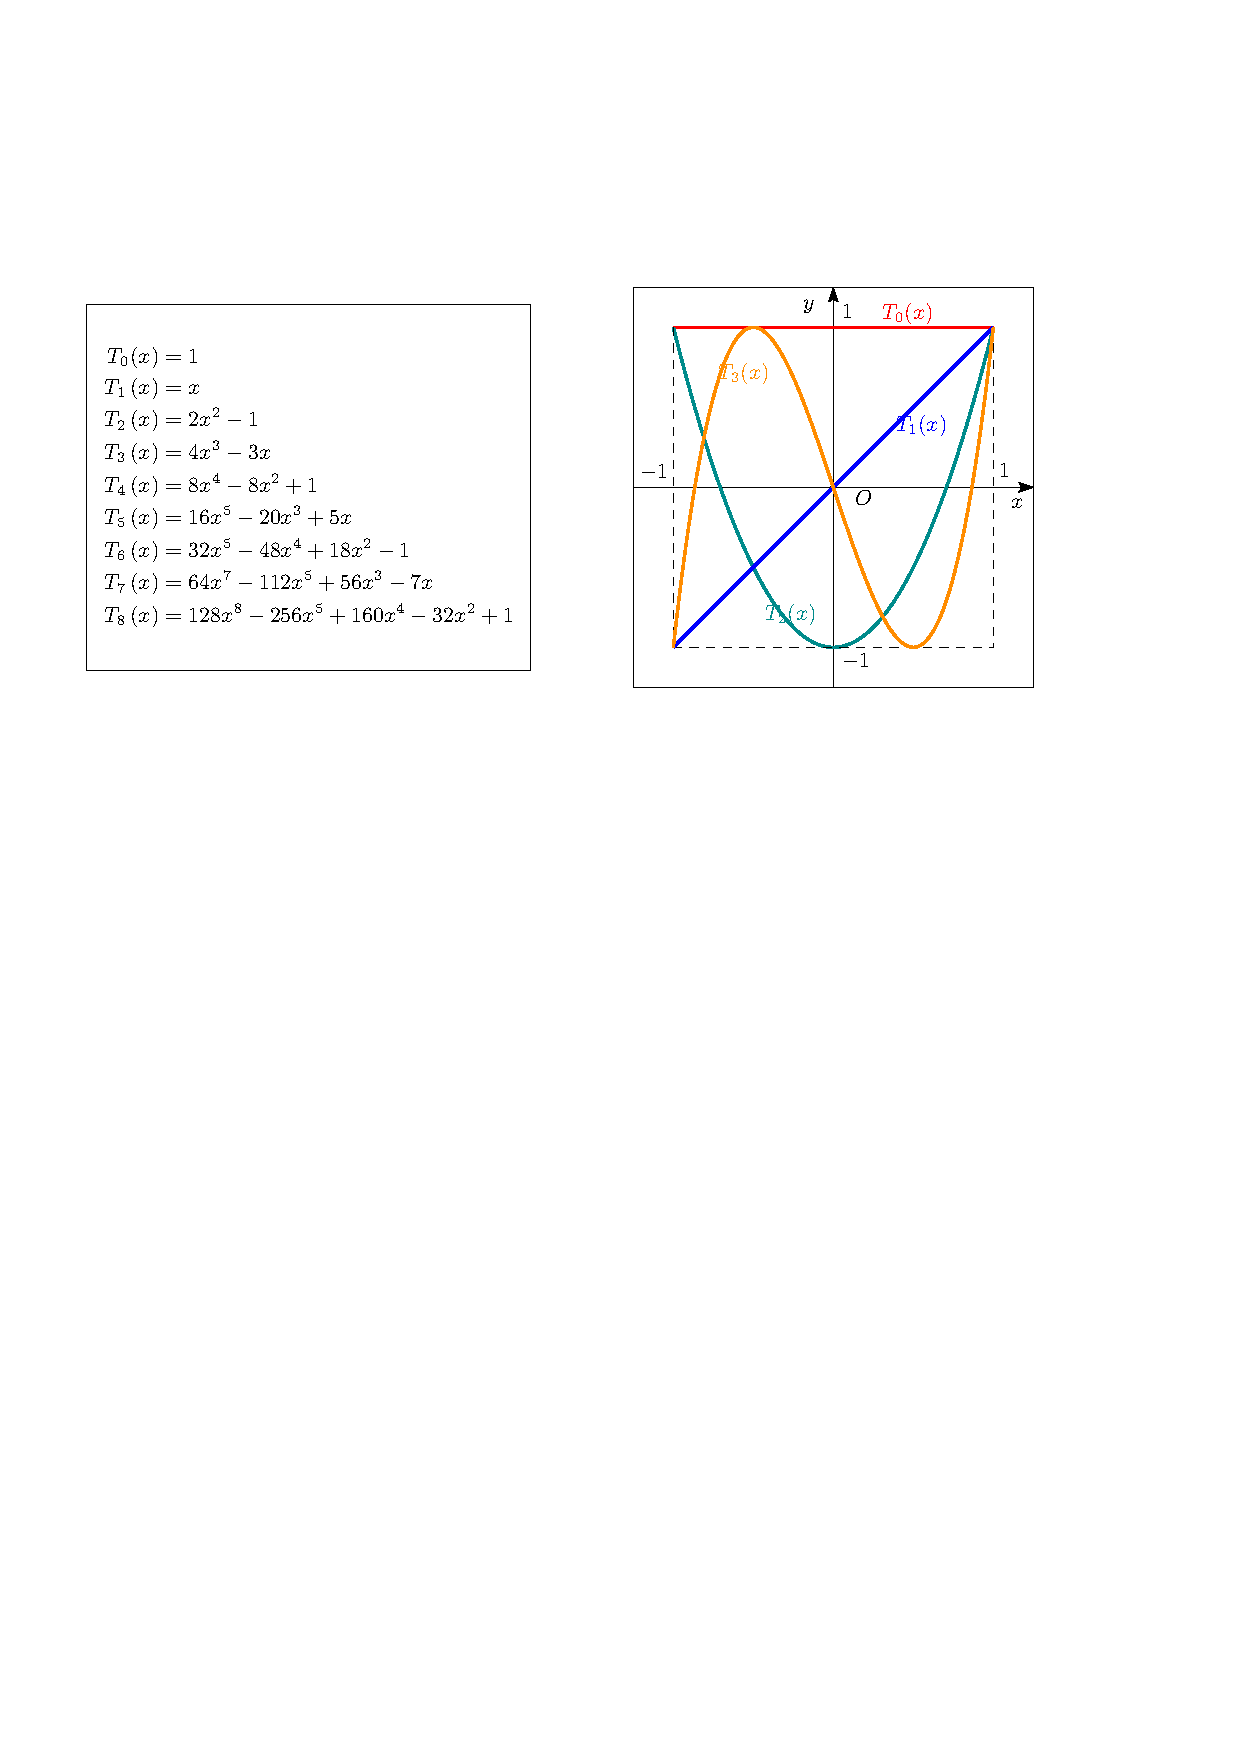
\includegraphics[width = .86\textwidth]{image/ChebyshevTx.pdf}
    \end{figure}
\end{note}
\begin{note}
    性质:
    \begin{enumerate}
        \item 正交性
        \[
            (T_n,T_m)=\begin{cases}
                0&m\neq n\\
                \dfrac{\pi}{2}& m=n\neq 0\\
                \pi & m=n=0
            \end{cases}
        \]
        \item 递推关系$T_{n+1}(x) = 2xT_{n}(x) + T_{n-1}(x)$
        \item 奇偶性$T_n(-x)=(-1)^nT_n(x)$
    \end{enumerate}
\end{note}
\begin{example}
    设$f(x) = x^4$,在$[-1,1]$上求$H_3$中的最佳逼近多项式。\Stars{3.5}{}

    \begin{solution}
        由定理~\ref{theo:Tx-0min}知道
        \[
            \dfrac{f(x)-p_{3}^{*}(x)}{1} = \dfrac{T_{4}(x)}{2^{4-1}}    
        \]
        其中$T_{4}\left(x\right) =8x^4-8x^2+1$,故而
        \[
            \begin{array}{ll}
                p_{3}^{*}(x) &= f(x)- \dfrac{T_{4}\left(x\right)}{2^{3}}\\
                &=x^2-\dfrac{1}{8}
            \end{array}
        \]
    \end{solution}
\end{example}
\begin{example}
    求$f(x) = 2x^3+x^2+2x-1$在$[-1,1]$上的最佳一致逼近多项式。\Stars{4}

    \begin{solution}
        \[
            \colorbox{red!30}{$\dfrac{f(x)-p_{2}^{*}(x)}{a_n}$} = \dfrac{T_{3}(x)}{2^{n-1}}\colorbox{red!30}{变成最高次系数为1的多项式}
        \]
        故
        \[
            p_{2}^{*}(x) = f(x)-\dfrac{1}{2}T_{3}(x) = x^2+\frac{7}{2}x-1
        \]
    \end{solution}
\end{example}
\begin{theorem}
    若$P(x)\in H_{n}$是$f(x)\in C[a,b]$的最佳逼近多项式,则$P(x)$同时存在正负偏差点。
\end{theorem}
\begin{theorem}[Chebyshev]\label{theo:Chebyshev}
    $p_n^*\in H_n$是$f\in C\left[ a,b \right]$的最佳逼近多项式的充要条件是:在$\left[ a,b \right]$上至少有$n+2$个轮流为正负的偏差点,即至少有$n+2$个点$a\leqslant x_1\leqslant x_2\leqslant \cdots\leqslant x_{n+2}\leqslant b$使得
    \[
        p_{n}^{*}(x_k)-f(x_k) = (-1)^{k}\sigma\| f-p_{n}^* \|_{\infty},\,\sigma = \pm 1,\,k =1,2,\cdots,n+2 
    \]
    上述点$\left\{ x_k \right\}_{1}^{n+2}$称为切比雪夫交错点。
\end{theorem}
\begin{corollary}
    设$f\in C[a,b]$,则在$H_n$中的最佳逼近多项式是唯一的。
\end{corollary}
\begin{corollary}
    若$f\in C[a,b]$,则其最佳逼近多项式$p_{n}^{*}(x)\in H_n$是$f$的一个拉格朗日多项式。
\end{corollary}
\begin{example}
    假定$f(x)\in C^{2}[a,b]$,且$f^{\prime\prime}(x)$在$(a,b)$内不变号,求最佳一次逼近多项式$P_1(x) = a_0+a_1x$。\Stars{5}{}
    \begin{solution}
        根据定理~\ref{theo:Chebyshev}可知,至少有3个点$a\leqslant x_1\leqslant x_2\leqslant x_3\leqslant b$使得
        \[
            P_{1}(x_k)-f(x_k) = (-1)^{k}\sigma\max\limits_{a\leqslant x\leqslant b}|P_{1}(x)-f(x)|
        \]
        由于$f^{\prime\prime}(x)$在$(a,b)$内不变号,故$f'(x)$单调,$f'(x)-a_1$在$(a,b)$内只有一个零点,记为$x_2$,于是
        \[
            P'_{1}(x_2)-f'(x_2) = a_1-f'(x_2) = 0,\quad\text{即}\,f'(x_2) = a_1
        \]
        \colorbox{red!50}{另外两个偏差点必在区间端点},即$x_0 = a,x_1  =b$,且满足
        \[
            P_{1}(a)-f(a) = P_{1}(b)-f(b) = -[P_{1}(x_2)-f(x_2)]
        \]
        由此得到
        \[
            \left\{
                \begin{array}{l}
                    a_0+a_1a-f(a)=a_0+a_1b-f(b)\\
                    a_0+a_1a-f(a)=f(x_2)-(a_0+a_1x_2).
                \end{array}
            \right.
        \]
        解得
        \[
            \begin{array}{l}
                a_1 = \dfrac{f(b)-f(a)}{b-a} = f'(x_2)\\
                a_0 = \dfrac{f(a)+f(x_2)}{2}-\dfrac{f(b)-f(a)}{b-a}\dfrac{a+x_2}{2}
            \end{array}
        \]
    \end{solution}
\end{example}
\begin{example}
    $f(x) = \sqrt{x^2+1}$,求$[0,1]$上的最佳一次逼近多项式。\Stars{2.5}
    
    \begin{solution}
        先求$x_2$和$f(x_2)$
        \[
            \begin{array}{l}
                f'(x_2) = \dfrac{x_2}{\sqrt{x_2^2+1}} = \dfrac{f(1)-f(0)}{1-0} = \sqrt{2}-1\approx 0.414\\
                \Rightarrow x_2  = \sqrt{\dfrac{\sqrt{2}-1}{2}}\approx 0.4551,\,f(x_2) = \sqrt{1+x_2^2} = 1.0986
            \end{array}
        \]
    \end{solution}
\end{example}
\subsection{最佳平方逼近}
\begin{definition}[正交函数]
    若$f(x),g(x)\in C[a,b]$满足
    \[
        (f,g) = \int_{a}^{b}\rho(x)f(x)g(x)\mathrm{d} x = 0,
    \]
    则称$f$与$g$在$[a,b]$上带权$\rho(x)$正交。若函数族$
    \varphi_{0}(x),\cdots,\varphi_{n}(x)$满足关系
    \[
        (\varphi_j,\varphi_k)=\int_a^b\rho(x)\varphi_j(x)\varphi_k(x)\mathrm{d}x=
        \left\{
            \begin{array}{ll}
                0, & j\neq k,\\
                A_k>0, & j=k,
            \end{array}
        \right.
    \]
    则称${\varphi_k}$是$[a,b]$上带权$\rho(x)$得正交族函数。
\end{definition}
\begin{theorem}
    若$(f,g)\in C[a,b]$,则有
    \[
        \begin{array}{ll}
            |(f,g)|\leqslant\|f\|_2\|g\|_2 & \text{柯西不等式} \\
            \parallel f+g\parallel_2\leqslant\parallel f\parallel_2+\parallel g\parallel_2 & \text{三角不等式} \\
            \parallel f+g\parallel_2^2+\parallel f-g\parallel_2^2=2(\parallel f\parallel_2^2+\parallel g\parallel_2^2) & \text{平行四边形定律} 
        \end{array}
    \]
\end{theorem}
\begin{definition}[最佳平方逼近函数]
    设$f\in [a,b]$,若$\exists \varphi^*\in\Phi = \operatorname*{Span}\{\varphi_0,\cdots,\varphi_n  \}$使得
    \[
        \| f-\varphi^* \|_2^2 = \inf\limits_{\varphi\in\Phi}\| f-\varphi \|_2^2
    \]
    则称$\varphi^*$为$f$在$\Phi$中的最佳平方逼近函数。
\end{definition}
\begin{note}
    上述问题等价于求多元函数
    \[
        I(a_0,a_1,\cdots,a_n) = \int_{a}^{b}\rho(x)\left[ \sum\limits_{j = 0}^{n}a_{j}\varphi(x)-f(x) \right]^2\mathrm{d}x
    \]
    的最小值。由于$I(a_0,a_1,\cdots,a_n)$是关于$a_0,a_1,\cdots,a_n$的二次函数,利用多元函数极值的必要条件
    \[
        \dfrac{\partial I}{\partial a_k}=2\int_a^b\rho(x)\Big[\colorbox{cyan!50}{$\sum_{j=0}^na_j\varphi_j(x)$}-\colorbox{red!50}{$f(x)$}\Big]\varphi_{k}(x)\mathrm{d}x=0,\quad(k=0,1,\cdots,n),
    \]
    \[
        \int_a^b\rho(x)\varphi_k(x)\sum_{j=0}^na_j\varphi_j(x)\mathrm{d}x= \int_a^b\rho(x)f(x)\varphi_k(x)\mathrm{d}x,\quad(k=0,1,\cdots,n),
    \]
    于是有\colorbox{red!50}{法方程}
    \[
        \sum\limits_{j = 0}^n(\varphi_j,\varphi_k)a_{j} = (f,\varphi_k),k = 0,\cdots,n
    \]
    系数矩阵$\boldsymbol{A}$为
    \[
        \boldsymbol{A} = 
        \begin{bmatrix}
            (\varphi_0,\varphi_0) & (\varphi_0,\varphi_1) & \cdots & (\varphi_0,\varphi_n) \\
            (\varphi_1,\varphi_0) & (\varphi_1,\varphi_1) & \cdots & (\varphi_1,\varphi_n) \\
            \vdots & \vdots & \ddots & \vdots \\
            (\varphi_n,\varphi_0) & (\varphi_n,\varphi_1) & \cdots & (\varphi_n,\varphi_n)
        \end{bmatrix}
    \]
\end{note}
\begin{example}
    设$f(x) = \sqrt{1+x^2}$,求$[0,1]$上的一次最佳平方逼近多项式$p_1^*(x) = a_0^*+a_1^*x$\Stars{5}{}
    
    解:
    系数:
    \[
        (\varphi_0,\varphi_0) = 1,\quad (\varphi_0,\varphi_1) = \dfrac{1}{2},\quad(\varphi_1,\varphi_1) = \dfrac{1}{3}
    \]
    \[
        (f,\varphi_0) = \int_{0}^{1}f(x)\cdot 1\mathrm{d} x,\quad (f,\varphi_1) = \int_{0}^{1}f(x)\cdot x\mathrm{d} x
    \]
\end{example}
\subsection{正交多项式}
若取$\left\{ \varphi_k(x) \right\}_{k = 0}^{n}$为正交多项式族,求$f$在$\Phi = \operatorname{Span}\left\{ \varphi_0,\varphi_1,\cdots,\varphi_n \right\}$上的最佳平方逼近,此时\colorbox{red!50}{法方程}的的系数矩阵\colorbox{red!50}{$\boldsymbol{A}$}为\colorbox{cyan!50}{对角阵}。
\[
    a_k^*=\frac{(f,\varphi_k)}{(\varphi_k,\varphi_k)},\quad k=0,1,\cdots n
\]
\begin{definition}[正交多项式族]
    若$\varphi_n$是首项次数$a_n\neq 0$的$n$次多项式,若
    \[
        (\varphi_i,\varphi_j)=\int_a^b\varphi_i\varphi_j\rho(x)dx = \left\{
            \begin{array}{lr}
                0 & i\neq j \\
                A_{i}\neq 0 & i = j
            \end{array}
        \right.
    \]
    则称多项式族序列$\left\{ \varphi_i \right\}_{0}^{\infty}$是在$[a,b]$上带权$\rho(X)$的正交多项式族,$\varphi_n$是在$[a,b]$上带权$\rho$的正交多项式序列。
\end{definition}
\begin{definition}[施密特正交化]
    $x^n$减去投影到$1,\cdots,x^{n-1}$方向的分量:
    \begin{itemize}
        \item $\dfrac{(x^n,\varphi_k)}{\| \varphi_k \|_2}$:$x^n$投影到$\varphi_k$方向的长度
        \item $\dfrac{\varphi_k}{\| \varphi_k \|_2}$:$\varphi_k$方向的单位向量
    \end{itemize}
    序列$\left\{ x^n \right\}_{0}^{\infty}$\colorbox{cyan!50}{线性无关且正交}。
    \[
        \varphi_0(x)=1,\quad\varphi_n(x)=x^n-\sum_{k=0}^{n-1}\frac{(\colorbox{cyan!50}{$x^n$},\colorbox{red!50}{$\varphi_k$})}{(\colorbox{cyan!50}{$\varphi_k$},\colorbox{red!50}{$\varphi_k$})}\colorbox{red!50}{$\varphi_k$}
    \]
\end{definition}
\begin{theorem}
    设$\{\varphi_{n}\}_{0}^{\infty}$在$[a,b]$上带权$\rho$的正交多项式序列,则$\varphi_n(n\geqslant 1)$的$n$个根都是单重实根,且都在$(a,b)$内。
\end{theorem}
\begin{proof}
    设$\varphi_{n}(x)$有$m$个奇数重根($m\leqslant n$),记为$x_1,\cdots,x_m$,证明上述定理就是证明$m = n$。

    记
    \[
        q(x) = (x-x_1)\cdots(x-x_m)
    \]
    那么$\varphi_{n}(x) q(x)$在$(a,b)$内不变号,
    \[
        (\varphi_{n}(x), q(x)) = \int_{a}^{b}\varphi_{n}(x) q(x)\mathrm{d}x\neq 0
    \]
    
    \colorbox{cyan!50}{因为($q(x)$可以表示为正交多项式序列$\{\varphi_{n}\}_{0}^{n}$的线性组合)},那么若$m<n$,则$(\varphi_{n}(x), q(x)) = 0$。故而$m = n$,即$\varphi_{n}(x)$有$n$个单根。证毕!
\end{proof}

\begin{definition}[勒让德( Legendre )多项式]
    区间为$[-1,1]$和权函数为$\rho = 1$,由$\{1,x,\cdots\}$正交化得到的多项式称为Legendre多项式。
    
    下面试着写几个Legendre多项式
    \begin{itemize}
        \item $P_{0}(x) = 1$
        \item $P_{1}(x) = x$
        \item $P_{2}(x)$
        \[
            \begin{aligned}
                P_{2}(x) & =x^2-\dfrac{(x^2,1)}{(1,1)}\cdot 1-\dfrac{(x^2,x)}{(x,x)}\cdot x\\
                &=x^2-\dfrac{\int_{-1}^{1}x^2\cdot 1\mathrm{d}x}{\int_{-1}^{1}1\cdot 1\mathrm{d}x}\cdot 1-\dfrac{\int_{-1}^{1}x^2\cdot x\mathrm{d}x}{\int_{-1}^{1}x\cdot x\mathrm{d}x}\cdot x\\
                &=x^2-2\dfrac{1/3}{2}-\dfrac{0}{2/3}x = x^2-\dfrac{1}{3}
            \end{aligned}
        \]
    \end{itemize}
    通项可以写为
    \[
        P_{0}(x)=1,P_{n}(x)=\frac{1}{2^{n}n!}\frac{\mathrm{d}^{n}}{\mathrm{d}x^{n}}\{(x^{2}-1)^{n}\},n=1,2,\cdots 
    \]
\end{definition}
\begin{corollary}
    Legendre多项式有以下性质
    \begin{enumerate}
        \item 正交性
        \[
            (P_m,P_n) = \left\{
                \begin{array}{ll}
                    0, & m\neq n \\
                    \dfrac{2}{2n+1}, & m = n
                \end{array}
            \right.
        \]
        \item 递推关系
        \[
            (n+1)P_{n+1}(x) = (2n+1)xP_{n}(x)-nP_{n-1}(x),\quad n = 1,2,\cdots
        \]
        \item 奇偶性
        \[
            P_{n}(-x) = (-1)^{n}P_{n}(x)
        \]
    \end{enumerate}
\end{corollary}
\begin{theorem}
    在所有首项系数为1的$n$次多项式中,Legendre多项式$\tilde{P}_{n}(x)$在$[-1,1]$上与零的平方误差最小。
\end{theorem}
\begin{proof}
    设$Q_{n}(x)$是首项系数为1的$n$次的多项式
    \[
        Q_{n}(x) = \tilde{P}_{n}(x)+\sum\limits_{k = 1}^{n}a_k\tilde{P}_{k}(x)    
    \]
    \[
        \begin{array}{ll}
            \|Q_{n}(x)\|_2^2 &= (Q_{n}(x),Q_{n}(x))\\
            &=(\tilde{P}_{n}(x)+\sum\limits_{k = 1}^{n-1}a_k\tilde{P}_{k}(x),\tilde{P}_{n}(x)+\sum\limits_{k = 1}^{n-1}a_k\tilde{P}_{k}(x))\\
            &=(\tilde{P}_{n}(x),\tilde{P}_{n}(x))+\sum\limits_{k = 0}^{n-1}(a_k\tilde{P}_{k},a_k\tilde{P}_{k})\\
            & \geqslant \|\tilde{P}_{n}(x)\|_{2}^{2}
        \end{array}
    \]
    当且仅当$a_0 = a_1 = \cdots = a_{n-1} = 0$时取等号。证毕!
\end{proof}
\subsection{最小二乘法}
\begin{definition}[最小二乘问题]
    设$f$由函数表$(x_i,f_i),\ i = 1,2,\cdots,m$给出,求$\varphi^{*}\in\Phi=\mathrm{Span}\{\varphi_{0},\cdots,\varphi_{n}\},n<m,$使
    \[
        \parallel f-\varphi^*\parallel_2^2=\sum_{i=0}^m[f_i-\varphi^*(x_i)]^2\rho_i=\inf_{\varphi\in\Phi}\parallel f-\varphi\parallel_2^2
    \]
    就是曲线拟合的最小二乘问题,称$\varphi^*(x)$为$f$在$\Phi$中的最小二乘逼近函数。
\end{definition}

求解上述问题也就是求
\[
    \begin{pmatrix}
        a_{11}&a_{12}&\cdots&a_{1n}\\
        a_{21}&a_{22}&\cdots&a_{2n}\\
        \vdots&\vdots&\ddots&\vdots\\
        a_{m1}&a_{m2}&\cdots&a_{nm}
    \end{pmatrix}
    \begin{pmatrix}
        x_1\\
        x_2\\
        \vdots\\
        x_n
    \end{pmatrix}=
    \begin{pmatrix}
        y_1\\
        y_2\\
        \vdots\\
        y_m
    \end{pmatrix}
\]
\[
    \begin{array}{l}
        \boldsymbol{Ax} = \boldsymbol{b}\colorbox{cyan!50}{无解}\\
        \colorbox{cyan!50}{投影到以$\boldsymbol{A}$的列向量为基的空间中}\\
        \boldsymbol{A}^{\mathrm{T}}\boldsymbol{Ax} = \boldsymbol{A}^{\mathrm{T}}\boldsymbol{b}
    \end{array}
\]
如图,在三维空间$O-xyz$中,$\overrightarrow{OA}=\boldsymbol{\alpha_1}$、$\overrightarrow{OB}=\boldsymbol{\alpha_2}$,$\overrightarrow{OP'}=\boldsymbol{b}$。显然无解,那么我们可以退而求其次找距离$\overrightarrow{OP'}$最近的解。
\begin{figure}[H]
    \centering
    % \pgfplotsset{compat=1.18}
\begin{tikzpicture}
    \begin{axis}[xlabel=$x$,ylabel=$y$,zlabel=$z$]
        \node(O) at (0,7,7){$O$};
        \node(A) at (0,60,50){$A$};
        \node(B) at (420,120,45){$B$};
        \node(P) at (240,120,45){$P$};
        \node(Q) at (240,120,80){$P'$};
        \addplot3 coordinates {(0,0,0) (0,0.5,0.5)};
        \addplot3 coordinates {(0,0,0) (0.5,1,0.5) };
        \addplot3 coordinates {(0,0,0) (0.25,1,1) };
        \addplot3 coordinates {(0,0,0) (0.25,1,0.5) };
        \addplot3 [surf] coordinates {
        (0,0,0) (0,1,1) (0.5,1,0.5) 
        };
        \addplot3 coordinates {(0.25,1,1) (0.25,1,0.5)};
    \end{axis}
\end{tikzpicture}  
\end{figure}

% !TeX program = xelatex*2
% !TeX root = ../elegantnote.tex
\section{数值积分与数值微分}
\subsection{数值积分基本概念}
数值积分就是将定积分的计算用\textcolor{cyan}{和式}近似表示
\[
    I = \int_{a}^{b}f(x)\mathrm{d}x \approx \sum\limits_{k = 0}^{n}A_kf(x_k)
\]
其中$A_k$与被积函数$f$无关,称为求积系数,$x_k$为求积节点。

\begin{definition}[插值型求积公式]
    在$[a,b]$上给定$n+1$个节点$a\leqslant x_0\leqslant x_1\leqslant\cdots\leqslant x_n\leqslant b$,以及相应的函数值$f(x_0),\cdots f(x_n)$
    \[
        L_n(x) = \sum\limits_{k = 0}^{n}l_{k}(x)f(x_k)
    \]
    \[
        \begin{array}{ll}
            I &= \int_{a}^{b}f(x)\mathrm{d}x \approx  \int_{a}^{b} L_n(x)\mathrm{d}x\\
            &=\int_{a}^{b}\sum\limits_{k = 0}^{n}f(x_k)l_{k}(x)\mathrm{d}x=\sum\limits_{k = 0}^{n}\int_{a}^{b}f(x_k)l_{k}(x)\mathrm{d}x\\
            &=\sum\limits_{k = 0}^{n}f(x_k)\int_{a}^{b}l_{k}(x)\mathrm{d}x=\sum\limits_{k = 0}^{n}A_kf(x_k)
        \end{array}
    \]
    其中,$A_k = \int_{a}^{b}l_{k}(x)\mathrm{d} x$

    $n = 1$时,由
    \[
        \begin{aligned}
            I(f) &= \int_{a}^{b}\dfrac{x-b}{a-b}f(a) + \dfrac{x-a}{b-a}f(b)\mathrm{d}x \\
            &= \dfrac{1}{2}\dfrac{(x-b)^2}{a-b}f(a)\Big|_{a}^{b} + \dfrac{1}{2}\dfrac{(x-a)^2}{b-a}f(b)\Big|_{a}^{b}\\
            &=\colorbox{cyan!50}{$ \dfrac{b-a}{2}$}[f(a)+f(b)] 
        \end{aligned}
    \]
    $A_0 = A_1 = \colorbox{cyan!50}{$\dfrac{b-a}{2}$}$,
    该式称为\colorbox{cyan!50}{梯形公式}。
\end{definition}
\begin{example}
    设$P_2(x)$是以$0,h,2h$为插值点的$f(x)$的二次插值多项式,用$P_{2}(x)$导出计算积分$I = \int_{0}^{3h}f(x)\mathrm{d}x$的数值积分公式$I_h$。\Stars{3}{}
    \begin{solution}
        易知:
        \[
            \begin{array}{l}
                P_{2}(x) = \dfrac{(x-h)(x-2h)}{(0-h)(0-2h)}f(0) + \dfrac{(x-0)(x-2h)}{(h-0)(h-2h)}f(h)\\
                +\dfrac{(x-0)(x-h)}{(2h-0)(2h-h)}f(2h)\\
            \end{array}
        \]
        故而
        \[
            I_h = \left[ \dfrac{3}{2}f(0) + \dfrac{9}{2}f(2h) \right]h
        \]
    \end{solution}
\end{example}
\begin{definition}[求积公式的代数精确度]
    若求积公式
    \[
        I(f) = \sum\limits_{k = 0}^{n}A_{k}f(x_k)
    \]
    对$f(x) = 1,x,\cdots,x^m$时精确成立,而对$f(x) = x^{m+1}$不精确成立,则称求积公式具有$m$次代数精度。
    \begin{itemize}
        \item 当$f(x) = 1$时,$\sum\limits_{k = 0}^{n}A_{k} = \int_{a}^{b}\mathrm{d}x = b-a$
        \item 当$f(x) = x$时,$\sum\limits_{k = 0}^{n}A_{k}x = \int_{a}^{b}\mathrm{d}x = \dfrac{1}{2}(b^2-a^2)$
        \item ……
        \item 当$f(x) = x^m$时,$\sum\limits_{k = 0}^{n}A_{k}x^m = \int_{a}^{b}x^m \mathrm{d}x = \dfrac{1}{m+1}(b^{m+1}-a^{m+1})$
        \item 当$f(x) = x^{m+1}$时,$\sum\limits_{k = 0}^{n}A_{k}x^{m+1} \neq \int_{a}^{b}x^{m+1}\mathrm{d}x$
    \end{itemize}
    \colorbox{cyan!50}{$n+1$个点的插值型求积公式\textcolor{red}{至少}有$n$次代数精确度}
\end{definition}
\begin{theorem}
    求积公式$I(f) = \sum\limits_{k = 0}^{n}A_{k}f(x_k)$至少有$n$次代数精确度的充分必要条件是它是插值型的。
\end{theorem}
\begin{proof}
    由插值余项定理,可知
    \[
        R[f] = I-I_n = \int_{a}^{b}\dfrac{f^{n+1}(\xi)}{(n+1)!}w_{n+1}(x)\mathrm{d}x
    \]
    如果是插值型的,$R[f] = 0$。证毕!
\end{proof}
\begin{example}
    求积公式
    \[
        \int_0^1f(x)dx\approx A_0f(0)+A_1f(1)+B_0f'(0),
    \]
    已知其余项表达式为$R(f)= kf'''(\xi),\xi\in (0,1)$。试确定$A_0,A_1$及$B_0$,使该求积公式具有尽可能高的代数精确度,并给出代数精确度的次数及求积公式余项。\Stars{5}{}
    \begin{solution}
        \begin{itemize}
            \item 当$f(x) = 1$时,$A_0+A_1 = 1$
            \item 当$f(x) = x$时,$A_1+B_0 = \dfrac{1}{2}$
            \item 当$f(x) = x^2$时,$A_1 = \dfrac{1}{3}$
        \end{itemize}
        得到$A_0 = \dfrac{2}{3},A_1 = \dfrac{1}{3},B_0 = \dfrac{1}{6}$,
        公式的代数精确度为$2$。
        \newline 
        令$f(x) = x^3$,余项为
        \[
            \begin{aligned}
                R[f] =& \int_{0}^1 x^3\mathrm{d}x-\dfrac{2}{3}\cdot 0^3-\dfrac{1}{3}\cdot 1^3-\dfrac{1}{6}(3\cdot 0)^2\\
                -\dfrac{1}{12}&=3!\colorbox{cyan!50}{$f'''(\xi)$}
            \end{aligned}
        \]
        故而,$k = -\dfrac{1}{72}$。
    \end{solution}
\end{example}
\begin{example}
    确定求积公式中的待定系数$a$,使其代数精度尽量高,并指出其具有的代数精度及余项\Stars{5}{}
    \[
        \int_{0}^{h}f(x)\mathrm{d}x\approx \dfrac{h}{2}\left[ f(0)+f(h) \right]+ah^2\left[ f'(0)-f'(h) \right]
    \]
    \begin{solution}
        \begin{itemize}
            \item 当$f(x) = 1$时,$h = h+0$恒成立
            \item 当$f(x) = x$时,$\dfrac{h^2}{2} = \dfrac{h^2}{2}+0$恒成立
            \item 当$f(x) = x^2$时,$\dfrac{h^3}{3} = \dfrac{h^3}{2} + ah^2\cdot (-2h)$,得
            \[
                a = -\dfrac{1}{12}
            \]
            代数精度为$3$。
        \end{itemize}
    \end{solution}
\end{example}
\begin{definition}
    对任给$\varepsilon>0$,若$\exists \delta>0$,只要$|f(x_k)-\tilde{f}_{k}|\leqslant \delta(k = 0,1,\cdots,n)$就有
    \[
        |I_{n}(f)-I_{n}(\tilde{f}) = \left|\sum_{k=0}^{n}A_{k}(f(x_{k})-\widetilde{f}_{k})\right|\leqslant \varepsilon
    \]
    成立,则称求积公式是稳定的。
\end{definition}
\begin{theorem}
    若求积公式中系数$A_k>0(k = 0,1,\cdots, n)$,则此求积公式是稳定的。
\end{theorem}
\subsection{Newton-Cotes求积公式}
\begin{definition}[Newton-Cotes公式]
    考虑等间距剖分情况下的插值型求积公式,设等距节点:$x_k = a+kh$,其中$h = \dfrac{b-a}{n},\,k = 0,1,\cdots, n$。
    插值基函数$l_{k}(x)$为
    \[
        l_{k}(x) = \prod\limits_{\substack{j=0\\ j\neq k}}^{n}\dfrac{x-x_j}{x_k-x_j} = \prod\limits_{\substack{j=0\\ j\neq k}}^{n}\dfrac{t-j}{k-j}
    \]
    \[
        \mathrm{d}x = \dfrac{b-a}{n}\mathrm{d}t
    \]
    \[
        \begin{aligned}
            \int_a^bf(x)\mathrm{d}x  &\approx \sum_{k= 0}^{n}A_{k}f(x_k)  = \sum_{k= 0}^{n}f(x_k)\int_{a}^{b}l_{k}(x)\diff x \\
            & = \sum_{k= 0}^{n}f(x_k)\int_{0}^{n}\frac{b-a}{n}\prod\limits_{\substack{j=0\\ j\neq k}}^{n}\dfrac{t-j}{k-j}\diff t \\
            &= (b-a)\sum\limits_{k = 0}^nC_{k}^{(n)}f(x_k)+R_n[f]
        \end{aligned}
    \]
    其中,$C_k^{(n)}=\dfrac{1}{n}\int_{0}^{n}\prod\limits_{\substack{j=0\\ j\neq k}}^{n}\dfrac{t-j}{k-j}\mathrm{d}t$
\end{definition}
下面列出了一些Cotes系数
% Table generated by Excel2LaTeX from sheet 'Cotes系数'
\begin{table}[htbp]
    \centering
        \begin{tabular}{c|cccc}
            \hline
            $n$ & \multicolumn{4}{c}{$C_{k}^{(n)}$} \bigstrut\\
            \hline
            1   & $\frac{1}{2}$ & $\frac{1}{2}$ &     &  \bigstrut[t]\\
            2   & $\frac{1}{6}$ & $\frac{4}{6}$ & $\frac{1}{6}$ &  \\
            3   & $\frac{1}{8}$ & $\frac{3}{8}$ & $\frac{3}{8}$ & $\frac{1}{8}$ \bigstrut[b]\\
            \hline
        \end{tabular}%
\end{table}%  
\begin{theorem}
    当阶数$n$为偶数时,Newton-Cotes公式至少有$n+1$次代数精度。
\end{theorem}
\begin{note}
    梯形公式:

    \[
        \begin{aligned}
            &I(f) = \frac{b-a}{2}\left[ f(a)+f(b) \right] \\
            &E(f) = \int_{a}^{b}\dfrac{f''(\xi)}{2}(x-a)(x-b)\diff x = -\frac{(b-a)^3}{12}f''(\eta)
        \end{aligned} 
    \]
\end{note}
\begin{note}
    Simpson公式:

    \[
        \begin{aligned}
            &I(f) = \frac{b-a}{6}\left[ f(a)+4f(\frac{a+b}{2})+f(b) \right] \\
            &E(f) = -\frac{(b-a)^5}{2880}f^{(4)}(\eta)
        \end{aligned} 
    \]
\end{note}
\subsubsection{复化求积法及其收敛性}
\begin{definition}[复化求积公式]
    考虑等间距剖分情况下的插值型求积公式,设等距节点:$x_k = a+kh$,其中$h = \dfrac{b-a}{n},\,k = 0,1,\cdots, n$。先用低阶的Newton-Cotes公式求得每个子区间$[x_k,x_{k+1}]$上的积分值$I_k$然后再求和用作为所求分的近似值,然后再求和。
    \[
        \begin{array}{ll}
            \int_a^bf(x)dx & \approx T_n(f)\\
            &= \sum\limits_{k=0}^{n-1}\dfrac{h}{2}[f(x_k)+f(x_{k+1})] \\
            &=\dfrac{h}{2}[f(a)+2\sum\limits_{k=1}^{n-1}f(x_k)+f(b)]\\
        \end{array}
    \]
    其积分余项
    \[
        \begin{array}{ll}
            I-T_n&=\sum\limits_{k=0}^{n-1}\left[-\dfrac{h^3}{12}f^{\prime\prime}(\eta_k)\right]\\
            &= -\dfrac{h^3}{12}n\sum\limits_{k=0}^{n-1}\left[\dfrac{f^{\prime\prime}(\eta_k)}{n}\right] \\
            &=-\dfrac{b-a}{12}h^2f^{\prime\prime}(\eta).
        \end{array}
    \]
    \colorbox{cyan!50}{最后一个=这里用到连续函数介值定理}
    \newline
    这里称Simpson是2阶收敛的。
\end{definition}
\begin{note}
    梯形公式
    \[
        I_1(f)=\dfrac{b-a}{2}[f(a)+f(b)]\quad E_1(f)=-\dfrac{(b-a)^3}{12}f''(\eta)
    \]
    复合梯形公式
    \[
        \int_a^bf(x)dx\approx T_n(f)=\dfrac{h}{2}[f(a)+2\sum_{k=1}^{n-1}f(x_k)+f(b)]
    \]
    误差
    \[
        E_n(f)=-\frac{b-a}{12}h^2f''(\eta),\quad\eta\in(a,b)
    \]
\end{note}
\begin{note}
    Simpson求积公式
    \[
        I_{2}(f)=\frac{b-a}{6}[f(a)+4f(\frac{a+b}{2})+f(b)]\quad E_{2}(f)=-\frac{(b-a)^{5}}{2880}f^{(4)}(\eta)
    \]
    复合Simpson求积公式
    \[
        \int_{a}^{b}f(x)dx\approx S_{n}(f)=\frac{h}{6}[f(a)+4\sum_{k=0}^{n-1}f(x_{k+\frac{1}{2}})+2\sum_{k=1}^{n-1}f(x_{k})+f(b)]
    \]
    误差
    \[
        E_n(f)=-\dfrac{b-a}{2880}h^4f^{(4)}(\eta),\:\eta\in(a,b)
    \]
\end{note}
\begin{note}
    Romberg算法:
    \begin{itemize}
        \item 梯形公式,Simpson公式,Cotes公式的代数精度分别为1次,3次和5次
        \item 复化梯形、复化Simpson、复化Cotes公式的收敛阶分别为2阶、4阶和6阶
    \end{itemize}
\end{note}
\begin{definition}[求积公式收敛阶]
    若一种复化求积公式$I_{n}$当$h\to 0$时成立
    \[
        \frac{I-I_{n}}{h^{p}}\to C(C\neq 0)  
    \]
    则称求积公式$I_{n}$是$p$阶收敛的。
\end{definition}
\subsection{Romberg算法}
将定积分$I=\int_{a}^{b}f(x)=\mathrm{d}x$的积分区间$[a,b]$分割为$n$等份,复化梯形(Trapz)公式为
\[
    T_n=\dfrac{b-a}{2n}[f(a)+2\sum_{j=1}^{n-1}f(x_j)+f(b)]
\]
如果将$[a,b]$分割为$2n$等份,则
\[
    T_{2n}=\dfrac{b-a}{4n}[f(a)+2\sum_{j=1}^{n-1}f(x_j)+2\sum_{j=0}^{n-1}f(x_{j+\frac{1}{2}})+f(b)]
\]
\[
    T_{2n}=\frac12T_n+\frac{b-a}{2n}\sum_{j=0}^{n-1}f(x_{j+\frac12})
\]
\begin{note}
    递推得梯形公式
    \[
        \left\{
            \begin{array}{l}
                T_{0}(0) = \dfrac{b-a}{2}\left[ f(a)+f(b) \right] \\
                T_{0}(k) = \dfrac{1}{2}T_{0}(k-1) + \dfrac{b-a}{2^k}\sum\limits_{j = 0}^{2^{k-1}}f\left( a+(2j+1)\dfrac{b-a}{2^k} \right)
            \end{array}
        \right.
    \]
\end{note}
\begin{example}
    已知$S_{n}=n\sin\dfrac{\pi}{n}=\pi-\dfrac{\pi^{3}}{3!n^{2}}+\dfrac{\pi^{5}}{5!n^{4}}-\cdots,$,如果采用Richardson外推法来基于$S$,计算$\pi$的值,那么下列公式中的加权系数分别是多少?\Stars{5}{}
    \begin{solution}
        \begin{enumerate}
            \item $\pi\approx\alpha_{1}S_{3}+\alpha_{2}S_{6}$
            有
            \[
                \left\{
                    \begin{array}{l}
                        \alpha_1+\alpha_2 = 1\\
                        -\alpha_1/9-\alpha_2/36 = 0
                    \end{array}
                \right.
            \]
            解得:
            \[
                \alpha_1 = -\dfrac{1}{3},\alpha_2 =\dfrac{4}{3}
            \]
            \item $\pi\approx\beta_1S_3+\beta_2S_9$
            有
            \[
                \left\{
                    \begin{array}{l}
                        \alpha_1+\alpha_2 = 1\\
                        -\alpha_1/9-\alpha_2/81 = 0
                    \end{array}
                \right.
            \]
            解得:
            \[
                \beta_1 = -\dfrac{1}{8},\alpha_2 =\dfrac{9}{8}
            \]
        \end{enumerate}
    \end{solution}
\end{example}
\begin{example}
    外推加速公式\Stars{5}{}
    \[
        \lambda_{1}F(h) = a+a_1h^p+o(h^8)
    \]
    \[
        \lambda_{2}F(h) = a+a_1\left( \dfrac{h}{2} \right)^p+o(h^8)
    \]
    \begin{solution}
        \[
        \lambda_{1}F(h)+\lambda_{2}F(h) =( \lambda_{1}+ \lambda_{2})a + a_1h^p(\lambda_1+\dfrac{\lambda_2}{2^p})
        \]
        \[
            \left\{
                \begin{array}{l}
                    \lambda_1+\lambda_2 = 1\\
                    \lambda_1+\dfrac{\lambda_2}{2^p} = 0
                \end{array}
            \right.
        \]
        得到
        \[
            \left\{
                \begin{array}{l}
                    \lambda_1 = -\dfrac{1}{2^p-1} \\
                    \lambda_2 = \dfrac{2^p}{2^p-1}
                \end{array}
            \right.
        \]
    \end{solution}
\end{example}
\begin{example}
    由复化梯形公式得余项公式\Stars{5}{}
    \begin{solution}
        \[
            I(f)-T_{n} = -\dfrac{b-a}{12}h^2f''(\eta)
        \]
        有
        \[
            I(f)-T_{2n} = -\dfrac{b-a}{12}\dfrac{h^2}{4}f''(\eta)
        \]
        结合二者可以得到
        \[
            \left\{
                \begin{array}{l}
                    \lambda_1 T_{n} = \colorbox{red!50}{$\lambda_1$}I(f) + \colorbox{cyan!50}{$\lambda_1$}\cdot\left[ -\dfrac{b-a}{12}\colorbox{cyan!50}{$h^2$}f''(\eta) \right]\\
                    \lambda_2 T_{2n} = \colorbox{red!50}{$\lambda_2$}I(f) + \colorbox{cyan!50}{$\lambda_2$}\cdot\left[ -\dfrac{b-a}{12}\colorbox{cyan!50}{$\dfrac{h^2}{4}$}f''(\eta) \right]
                \end{array}
            \right.
        \]
        那么
        \[
            \left\{
                \begin{array}{l}
                    \colorbox{red!50}{$\lambda_1$}+\colorbox{red!50}{$\lambda_2$} = 1\\
                    -\colorbox{cyan!50}{$\lambda_1$}-\colorbox{cyan!50}{$\dfrac{1}{4}\lambda_2$} = 0
                \end{array}
            \right.
        \]
        解得
        \[
            \left\{
                \begin{array}{l}
                    \lambda_1 = -\dfrac{1}{3} \\
                    \lambda_2 = \dfrac{4}{3}
                \end{array}
            \right.
        \]
        可以得到外推加速公式
        \[
            I(f) \approx \dfrac{4}{3}T_{2n}-\dfrac{1}{3}T_{n}
        \]
    \end{solution}
\end{example}
\subsection{高斯(Gauss)公式}
考虑带权积分$I(f)=\int_{a}^{b}f(x)\rho(x)\mathrm{d}x$,寻找形如
\[
    I(f)\approx\sum_{k=0}^nA_kf(x_k)=I_n(f)    
\]
的求积公式使它具有最高的代数精确度。式中含有$2n+2$个待定参数$x_k,A_k(k= 0,1,\cdots,n)$适当选择这些参数,有可能使得求积公式具有$2n+1$次代数精度。
\begin{definition}[Gauss型求积公式]
    具有最高代数精度的插值型求积公式称为Gauss型求积公式,相应的求积节点$a\leqslant x_0, < x_1 <\cdots< x_n\leqslant b$称为Gauss点。
\end{definition}
当插值型节点个数比较多时,方程求解比较困难。因此我们可以先找出满足条件的插值节点(Gauss点)。
\begin{theorem}
    插值型求积公式的求积节点$\{x_k\}_{k = 0}^{n}$是高斯点的充要条件是: 在$[a,b]$上以这组节点为根的多项式$\omega_{n+1}(x)=(x-x_{0})(x-x_{1})\cdots(x-x_{n})$与任何次数$\leqslant n$的多项式$P(x)$带权$\rho(x)$正交,即
    \[
        \int_a^bP(x)\omega_{n+1}(x)\rho(x)dx=0
    \]
\end{theorem}
\begin{proof}
    先证明必要性:即$\{x_k\}_{k = 0}^{n}$是高斯点$\Rightarrow \int_{a}^{b}Q(x)\rho(x)\mathrm{d}x = 0$

    设$x_k$为Gauss点,那么有
    \[
        Q(x) = P(x)\omega_{n+1}(x)
    \]
    是次数不超过$(2n+1)$次的多项式,则
    \[
        \int_{a}^{b}Q(x)\rho(x)\mathrm{d}x = \sum_{k = 0}^{n}A_{k}\colorbox{cyan!50}{$Q(x_k)$} = 0
    \]
    前一个等号利用了高斯节点的定义,后面是因为$\omega_{n+1}(x_k) = 0$

    再证明充分性:即$\int_{a}^{b}P(x)\omega_{n+1}(x)\rho(x)\mathrm{d}x = 0\Rightarrow \int_{a}^{b}P_{2n+1}(x)\mathrm{d}x = \sum_{k = 0}^{n}A_kP_{2n+1}(x_{k})$

    设$P_{2n+1}(x)$是任意次数$\leqslant 2n+1$次的多项式
    \[
        P_{2n+1}(x) = P(x)\omega_{n+1}(x)+Q(x)        
    \]
    其中$P(x),Q(x)$是次数$\leqslant n$的多项式
    \[
        \begin{aligned}
            & \int_{a}^{b}P_{2n+1}(x)\mathrm{d}x\\
            & =\cancel{\int_{a}^{b}P(x)\omega_{n+1}(x)\rho(x)\mathrm{d}x}+\int_{a}^{b}Q(x) \mathrm{d}x\\
            &=0+\sum_{k = 0}^{n}A_kQ(x_{k}) = \sum_{k = 0}^{n}A_kP_{2n+1}(x_{k})
        \end{aligned}
    \]
    最后一个等号是因为$P(x_k)\colorbox{cyan!50}{$\omega_{n+1}(x_k)$} = 0$

    故公式有$2n+1$次代数精度。证毕!
\end{proof}
\begin{theorem}
    Gauss型求积公式的求积系数$A_{k}> 0(k = 0,1,\cdots,n)$
\end{theorem}
\begin{proof}
    设$\left\{ x_k \right\}$为高斯点,$l_{k}(x)$是$x_k$点时对应的拉格朗日插值基函数,那么有
    \[
        0<\int_{a}^bl_{k}^{2}(x)\rho(x)\mathrm{d}x = \sum\limits_{j =0}^{n}A_{j}l_{k}^{2}(x_j) = A_{k}
    \]
\end{proof}
\begin{corollary}
    Gauss型求积公式是稳定的。
\end{corollary}
\begin{theorem}
    设$f\in C[a,b]$,则Gauss型求积公式是收敛的,即
    \[
        \lim_{n\to\infty}I_n(f)=\int_a^bf(x)\rho(x)dx
    \]
\end{theorem}
\begin{proof}
    仅对$\rho(x) = 1$进行证明,因$f\in C[a,b]$,由Weierstrass定理知,对$\forall \varepsilon>0,\exists P_{n}(x)$,使得
    \[
        \| f(x)-P_{n}(x) \|_{\infty}<\varepsilon
    \]
    \[
        \begin{aligned}
            &\left|I_{n}(f)-\int_{a}^{b}f(x)\mathrm{d}x\right|\\
            &\leqslant\left| I_{n}(f)-I_{n}(P)+I_{n}(P)-\int_{a}^{b}f(x)\mathrm{d}x \right|\\
            &\leqslant \left| I_{n}(f)-I_{n}(P) \right|+\left|I_{n}(P)-\int_{a}^{b}f(x)\mathrm{d}x\right|
        \end{aligned}
    \]
    而
    \[
        \begin{aligned}
            \left| I_{n}(f)-I_{n}(P) \right| &\leqslant \sum_{k = 0}^{n}A_k\left|f(x_{k})-P(x_k)\right|\\
            &\leqslant \sum_{k = 0}^{n}A_{k}\| f-P_{n} \|_{\infty}=(b-a)\| f-P_{n} \|_{\infty}
        \end{aligned}
    \]
    又
    \[
        \begin{aligned}
            \left|I_{n}(P)-\int_{a}^{b}f(x)\mathrm{d}x\right|&\leqslant \int_{a}^b \left| P-f \right|\mathrm{d}x\\
            & \leqslant \| P-f \|_{\infty}(b-a)\\
        \end{aligned}
    \]
    证毕!
\end{proof}
\begin{theorem}
    Gauss-Legendre求积公式的余项
    \[
        R(x)=\frac{f^{(2n+2)}(\xi)}{(2n+2)!}\int_a^b\omega^2(x)\mathrm{d}x
    \]
\end{theorem}
\begin{example}
    利用Gauss-Legendre求积公式求在$[a,b]$区间内的求积公式
    \begin{solution}
        \[
            \int_{a}^{b}f(x)\mathrm{d}x \overset{x = \frac{b+a}{2}+\frac{b-a}{2}t}{=} \dfrac{b-a}{2}\int_{-1}^{1}F(t)\mathrm{d}t\approx\dfrac{b-a}{2}\sum_{k = 0}^{n}A_{k}F(t_k)
        \]
        高斯点$t_0,t_1,\cdots,t_n$时$P_{n+1}$的零点。
    \end{solution}
\end{example}
\begin{example}
    求两点Gauss-Legendre积分的求积公式,并用其计算\Stars{5}{}
    \[
        I = \int_{0}^{\frac{\pi}{2}}\sin x\mathrm{d}x
    \]

    \begin{solution}
        \[
            I =  \int_{0}^{\frac{\pi}{2}}\sin x\mathrm{d}x = \dfrac{\pi}{4}\int_{-1}^{1}\sin(\dfrac{\pi}{4} + \dfrac{\pi}{4}t)\mathrm{d}t
        \]
        \[
            t_0 = -\dfrac{1}{\sqrt{3}},\quad t_1 = \dfrac{1}{\sqrt{3}}
        \]
    \end{solution}
\end{example}
\begin{example}
    区间$[3,5]$上两点Gauss-Legendre公式的求积节点分别为\Stars{5}{}
    \begin{solution}
        \[
            x_0 = 4-\dfrac{1}{\sqrt{3}},x_{1} =4+\dfrac{1}{\sqrt{3}} 
        \]
    \end{solution}
\end{example}
\begin{note}
    Gauss-Chebyshev公式
    \[
        [-1,1],\rho = \dfrac{1}{\sqrt{1-x^2}}
    \]
    $T_{n}(x)$的零点为$x_{k} = \dfrac{2k-1}{2n}\pi,\quad k = 1,2,\cdots,n$
    \[
        \int_{-1}^{1}f(x)\dfrac{1}{\sqrt{1-x^2}}\mathrm{d}x\approx \dfrac{\pi}{n}\sum_{k = 1}^{n}f(x_k)
    \]
\end{note}
\subsubsection{固定部分节点的高斯型求积公式}
在实际应用中有时希望预先固定高斯型公式的一个或几个求积节点。
\begin{example}
    假设求积公式中$m$个节点固定,$n$个节点待定。\Stars{3.5}{}
    \newline
    则该公式的代数精确度为\colorbox{cyan!50}{[$2n+m-1$]}
\end{example}

\begin{note}
    采用自适应Simpson公式计算$I=\int_{a}^{a+h}f(x)\mathrm{d}x$
    \[
        \begin{aligned}
            &S_{1}(a,a+h)=\frac{h}{6}\biggl[f(a)+4f(a+\frac{h}{2})+f(b)\biggr] \\
            &I-S_{1}(a,a+h)=-\frac{h^{5}}{2880}f^{(4)}(\eta) \\
            &S_{2}=S_{1}(a,a+\frac{h}{2})+S_{1}(a+\frac{h}{2},a+h) \\
            &I-S_{2}(a,a+h)=-\frac{1}{2880}\biggl(\frac{h}{2}\biggr)^{5}f^{(4)}(\overline{\eta}) \\
            & S_1-S_2 =  \frac{1}{2880}\biggl(\frac{15}{16}\biggr)h^{5}f^{(4)}(\overline{\eta})\\
            &I-S_{2}(a,a+h)\mid\approx\frac{1}{15}\mid S_{1}(a,a+h)-S_{2}(a,a+h)\mid <\varepsilon
        \end{aligned}
    \]
    \begin{figure}[htbp]
        \centering
        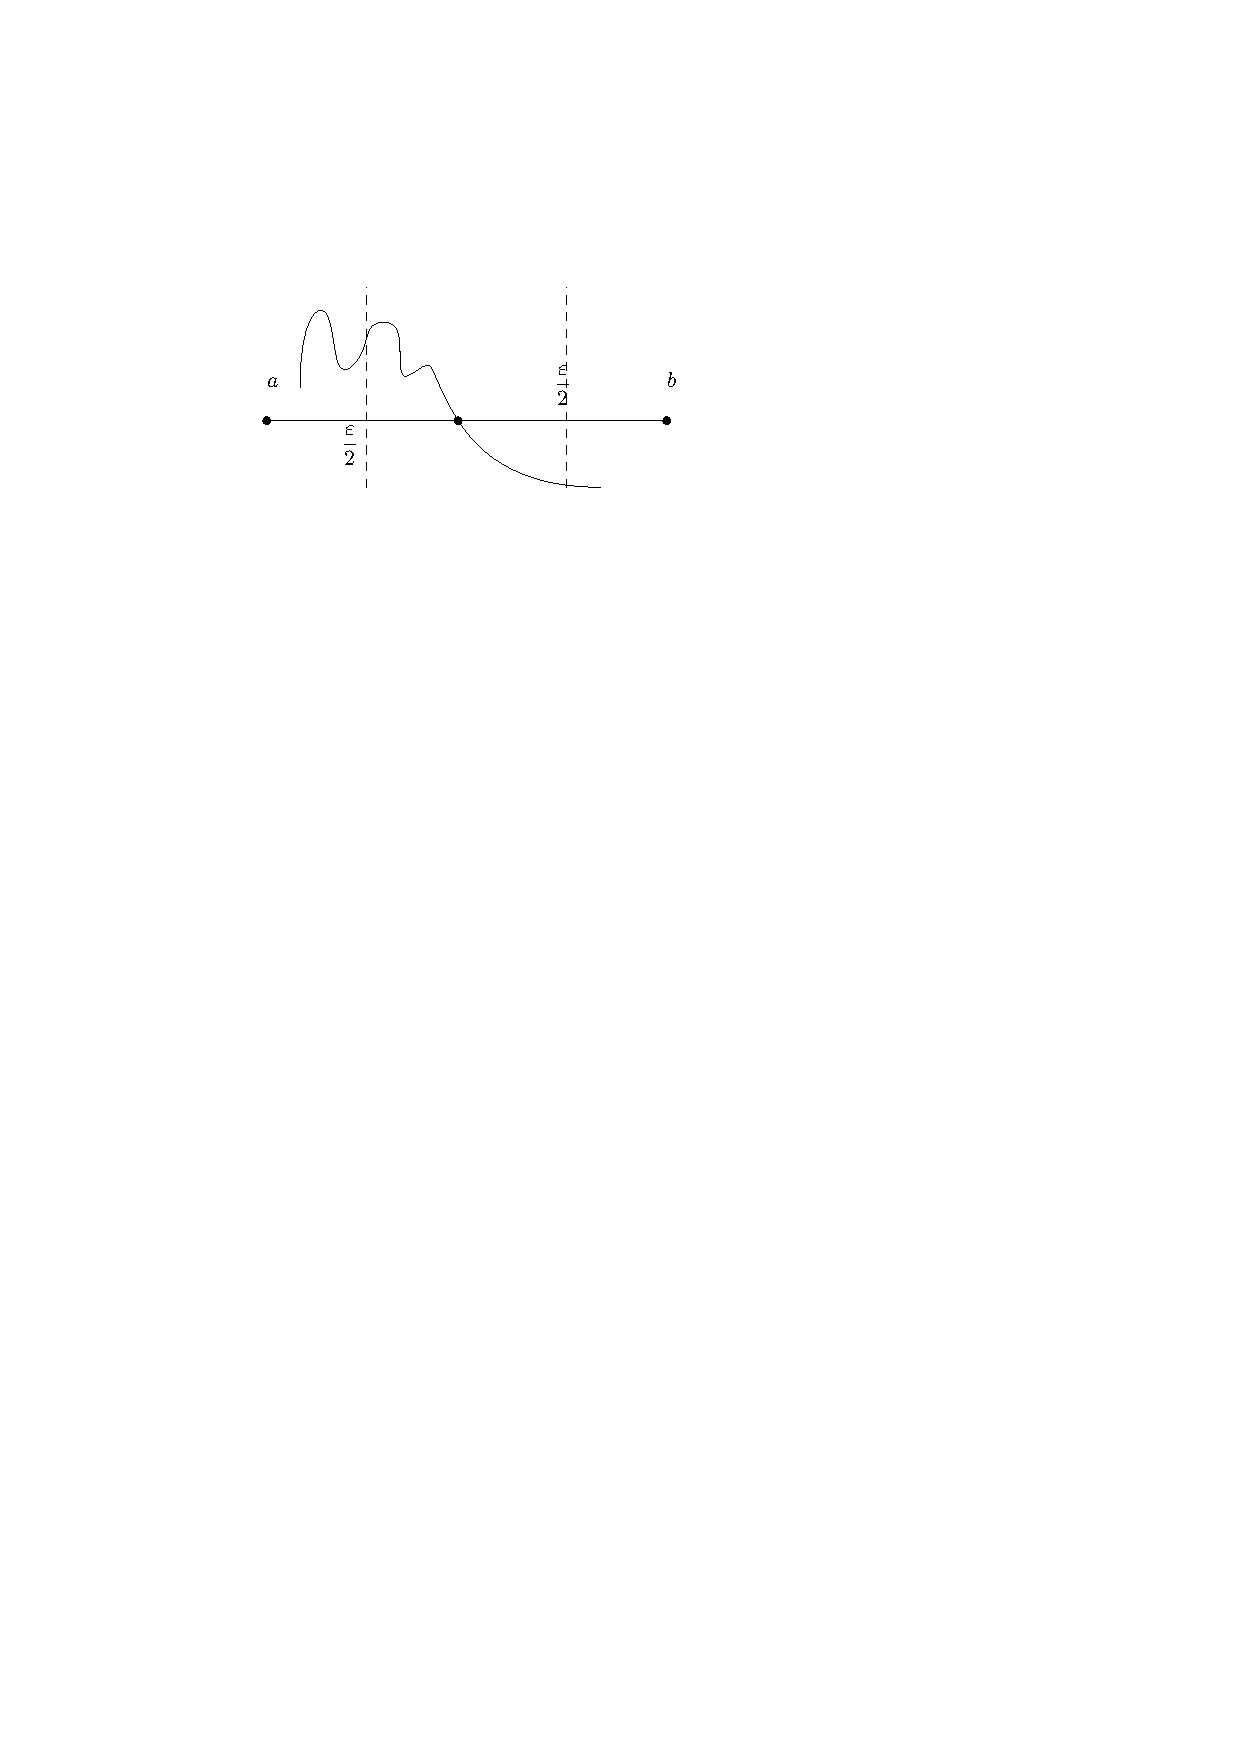
\includegraphics{image/自适应Simpson.pdf}
    \end{figure}
\end{note}
\subsection{二重积分计算方法}
\[
    \begin{aligned}
        I(f)&=\iint_{\Omega}f(x,y)dxdy\\
        & \int_a^b\mathrm{d}x\int_{\varphi(x)}^{\psi(x)}f(x,y)\mathrm{d}y = \int_{a}^{b}F(x)\mathrm{d}x \\
        & \approx\sum_{k = 0}^{n} A_{k}F(x_k)\\
        &\approx\sum_{k=0}^{n}A_{k}\left[\sum_{l=0}^{m}B_{kl}f(x_{k},y_{l})\right]
    \end{aligned}
\]

\begin{example}
    计算上述二重积分的梯形公式为
    \begin{solution}
        \[
            \begin{aligned}
                T(f)&=\frac{b-a}{2}[\frac{\psi(a)-\varphi(a)}{2}(f(a,\varphi(a))+f(a,\psi(a)))\\
                &+\frac{\psi(b)-\varphi(b)}{2}(f(b,\varphi(b))+f(b,\psi(b)))]
            \end{aligned}
        \]
    \end{solution}
\end{example}
\subsubsection{复合求积公式}
考虑矩形区域的重积分$\Omega=[a,b]\times[c,d]$
\[
    I(f)=\int_{a}^{b}\int_{c}^{d}f(x,y)\mathrm{d}x\mathrm{d}y
\]
\begin{note}
    复合梯形公式
    \[
        \begin{aligned}
            I(f)& =\iint_{\Omega}f(x,y)\mathrm{d}x\mathrm{d}y \\
            &\approx\frac{h_{x}h_{y}}{4}\sum_{i=0}^{n}\sum_{i=0}^{m}\lambda_{ij}f(x_{i},y_{j})
        \end{aligned}
    \]
    \[
        \Lambda=
        \begin{bmatrix}
            1&2&2&\cdots&2&2&1\\
            2&4&4&\cdots&4&4&2\\
            \vdots&\cdots&\vdots&\cdots&\cdots&\cdots\\
            2&4&4&\cdots&4&4&2\\
            1&2&2&\cdots&2&2&1
        \end{bmatrix}
        =(\lambda_{\mathbf{ij}})
    \]
\end{note}
\subsection{数值微分}
\subsubsection{机械求导公式}
\[
    f'(x_0) = \lim\limits_{h\to 0}\dfrac{f(x_0+h)-f(x_0)}{h}
\]
\[
    f'(x_0) \approx \dfrac{f(x_0+h)-f(x_0)}{h} = f'(x_0) + \dfrac{f''(x_0)}{2}h^2
\]
\begin{note}
    中点公式(二阶截断误差)
    \[
        G(h) = \dfrac{f(a+h)-f(a-h)}{2h}\quad \colorbox{cyan!50}{$h$过小,两相近的数相减,影响舍入误差}
    \]
    \[
        G(h) = f'(a) + \dfrac{h^2}{3!}f'''(a)+\dfrac{h^4}{5^!}f^{(5)}(a)+\cdots\quad \colorbox{red!50}{$h$小,截断误差小}
    \]
    \begin{itemize}
        \item \colorbox{cyan!50}{从舍入误差看,$h$不宜过小}
        \item \colorbox{red!50}{从截断误差看,$h$越小,计算越准确}
    \end{itemize}
\end{note}
\begin{example}
    以下关于数值微分的说法\colorbox{red!50}{不正确}的是 ()
    \begin{enumerate}
        \item[\choice{}{A}] 在实际应用中,基于插值多项式的微分方法,其插值次数不能太高
        \item[\choice{}{B}] 近似导数$f'(x)$的数值微分公式$\frac{f(x_{0}+h)-f(x_{0}-h)}{2h}$和$\frac{f(x_{0})-4f(x_{0}+h)+3f(x_{0}+2h)}{2h}$误差阶相同
        \item[\choice{}{C}] 数值微分公式的误差包括截断误差和舍入误差两部分
        \item[\choice{1}{D}] 当插值多项式$L_n(x)$收敛于$f(x)$时,其导数$L'_n(x)$收敛于$f'(x)$
    \end{enumerate}
\end{example}
\begin{definition}[插值型求导公式]
    建立$f(x)$的插值多项式$P_{n}(x)$,用$P'_{n}(x)$作为$f'(x)$的近似值
    \[
        f^{\prime}(x_{k})-P_{n}^{\prime}(x_{k})=\frac{f^{(n+1)}(\xi)}{(n+1)!}\omega_{n+1}^{\prime}(x_{k})
    \]
    其中$\omega_{n+1}^{\prime}(x_{k}) = (x-x_0)(x-x_1)(x-x_{k-1})\cdots(x-x_{k+1})(x-x_{n})$.

    两点公式:给定两个节点$x_0,x_1$,做线性插值多项式$P_{1}(x)$
    \[
        P_{1}^{\prime}(x_{0})=P_{1}^{\prime}(x_{1})=\frac{f(x_{1})-f(x_{0})}{h}
    \]
    \[
        f^{\prime}(x_{0})=P_{1}^{\prime}(x_{0})-\frac{h}{2}f^{\prime\prime}(\xi)\quad f^{\prime}(x_{1})=P_{1}^{\prime}(x_{1})+\frac{h}{2}f^{\prime\prime}(\xi)
    \]

    三点公式:给定三个节点$x_0,x_1,x_2$,做二次插值多项式$P_{2}(x)$
    \[
        P_{2}^{\prime}(x_{0})=\frac{-f(x_{2})+4f(x_{1})-3f(x_{0})}{2h}
    \]
    \[
        P_{2}^{\prime}(x_{1})=\frac{f(x_{2})-f(x_{0})}{2h}
    \]
    \[
        P_2'(x_2)=\frac{3f(x_2)-4f(x_1)+f(x_0)}{2h}
    \]
    以上公式近似相应导数的误差分别为$\frac{h^{2}}{3}f^{\prime\prime\prime}(\xi),-\frac{h^{2}}{6}f^{\prime\prime\prime}(\xi),\frac{h^{2}}{3}f^{\prime\prime\prime}(\xi).$
\end{definition}

% !TeX root = ../elegantnote.tex
\section{微分方程数值解的基本概念(没有大题)}
\subsection{微分方程数值解的基本概念}
\begin{theorem}
    如果方程$\begin{cases}\frac{dy}{dx}=f(x,y),\\y(x_0)=y_0.\end{cases}$中右端函数$f(x,y)$满足
    \begin{enumerate}
        \item $f(x,y)$是实值函数
        \item $f(x,y)$在矩形区域$\Omega=\{(x,y)|x\in[x_{0},T],y\in(-\infty,+\infty)\}$内连续
        \item $f(x,y)$关于$y$满足Lipschitz条件:即存在正常数$L$,使得对任意$x\in\left[ x_0,T \right]$,均成立不等式
        \[
            |f(x,y_1)-f(x,y_2)|\leq L|y_1-y_2|
        \]
    \end{enumerate}
    则方程存在唯一解$y(x)\in C^{1}[x_0,T]$
\end{theorem}
\begin{definition}[扰动问题]
    考虑扰动问题$\begin{cases}\dfrac{\mathrm{d}y}{\mathrm{d}x}=f(x,y)+\delta(x),x_0\leq x\leq T,\\y(x_0)=y_0+\varepsilon.\end{cases}$
\end{definition}
\begin{example}
    以下初值问题是否关于数据的扰动稳定?
    \[
        \begin{cases}
            \dfrac{\mathrm{d}u}{\mathrm{d}t}=100u-101e^{-t}\\
            u(0)=1
        \end{cases}
    \]
    \begin{enumerate}
        \item [\choice{}{A}] 是
        \item [\choice{1}{B}] 否 
    \end{enumerate}
    \begin{solution}
        原问题的通解为
        \[
            \begin{aligned}
                u(t) &= e^{-\int-100\mathrm{d}t}\left( \int -101e^{-t}e^{\int-100\mathrm{d}t}\mathrm{d}t + C \right)\\
                &=e^{100t}\left( e^{-101t} + C \right)
            \end{aligned}
        \]
        代入初始条件$u(0) = 1$得到
        \[
            u(t) = e^{-t}
        \]
        现在有初值的扰动$u(0) = 1+\varepsilon$得到
        \[
            u(t) = e^{-t} + \varepsilon e^{100t}
        \]
        显然对$\forall \varepsilon>0,u(t;\varepsilon)$偏离真解很大,故问题不稳定。
    \end{solution}
\end{example}
\subsection{Euler方法}
\begin{definition}[Euler方法]
    考虑问题
    \[
        \begin{cases}
            \dfrac{\mathrm{d}y(x)}{\mathrm{d}x}=f(x,y(x)),x_0\leq x\leq T,\\
            y(x_0)=y_0.
        \end{cases}
    \]
    将区域$\left[ x_0,T \right]$剖分成$m$等份,步长$h = \dfrac{T-x_0}{m},$网点$x_{n}=x_{n-1}+h=x_{0}+(n-1)h,n=1,2,\cdots,m.$
\end{definition}

\begin{note}
    梯形法
    \[
        y(x_{n+1})=y(x_{n})+\frac{h}{2}[f(x_{n},y(x_{n}))+f(x_{n+1},y(x_{n+1}))]+R_{n}^{(1)}
    \]
    \[
        R_{n}^{(1)}=-\frac{h^{3}}{12}y^{\prime\prime\prime}(\xi),x_{n}<\xi<x_{n+1}
    \]
    \[
        y_{n+1}=y_{n}+\frac{h}{2}[f(x_{n},y_{n})+f(x_{n+1},y_{n+1})]
    \]
    \begin{itemize}
        \item 梯形法为二阶方法
        \[
            \mid y(x_n)-y_n\mid=O(h^2),\text{当}h\to 0\text{时}  
        \]
        \item 梯形法为单步隐式方法
        \item 梯形法计算格式
        \[
            \begin{cases}
                y_{n+1}^{(0)}=y_{n}+hf(x_{n},y_{n}),\\
                y_{n+1}^{(m+1)}=y_{n}+\dfrac{h}{2}[f(x_{n},y_{n})+f(x_{n+1},y_{n+1}^{(m)})],\\
                m=0,1,2,\cdots
            \end{cases}
        \]
        \item \colorbox{cyan!50}{梯形格式收敛的条件}是什么?
        \[    
            y_{n+1}^{*} = y_n+\dfrac{h}{2}\left[ f(x_n,y_n)+f(x_{n+1},y_{n+1}^{*}) \right]
        \]
        记$y_{n+1}^{(m)}-y_{n+1}^{*} = \varepsilon^{m}$,则
        \[
            \begin{aligned}
                |\varepsilon^{(m+1)}| &= \dfrac{h}{2}\left[ f(x_{n+1},y_{n+1}^{(m)})+f(x_{n+1},y_{n+1}^{*}) \right]\\
                &\leqslant \dfrac{hL}{2}|y_{n+1}^{(m)}-y_{n+1}^{*}| = \dfrac{hL}{2}\varepsilon^{(m)}\\
                &=\left( \dfrac{hL}{2} \right)^{m}\varepsilon^{(0)}
            \end{aligned}
        \]
        \[
            \lim_{m\to \infty}|\varepsilon^{(m+1)}|\Longrightarrow\colorbox{cyan!50}{$\dfrac{hL}{2}<1$}
        \]
    \end{itemize}
\end{note}
\begin{example}
    下列关于梯形法的叙述错误的是\Stars{3}{}
    \begin{enumerate}
        \item [\choice{1}{A}]梯形法是一个显式方法
        \item [\choice{1}{B}]梯形法的整体截断误差是$O(h^3)$
        \item [\choice{}{C}]梯形法是一个稳定的方法
        \item [\choice{1}{D}]梯形法的迭代步长可以任取
    \end{enumerate}
\end{example}
\begin{note}
    改进Euler法
    \[
        \begin{cases}
            \overline{y}_{n+1}=y_n+hf(x_n,y_n)&\text{\textcolor{red}{预测}}\\
            y_{n+1}=y_n+\frac{h}{2}[f(x_n,y_n)+f(x_{n+1},\overline{y}_{n+1})]&\text{\textcolor{red}{校正}}
        \end{cases}
    \]
    预测校正格式还可写为
    \[
        y_{n+1}=y_n+\dfrac{h}{2}\Big[f(x_n,y_n)+f(x_n+h,y_n+hf(x_n,y_n))\Big]
    \]
    \[
        \begin{cases}
            y_p=y_n+hf(x_n,y_n)\\
            y_c=y_n+hf(x_{n+1},y_p)\\
            y_{n+1}=\dfrac{1}{2}[y_n+y_p]
        \end{cases}
    \]
\end{note}
\begin{example}
    改进Euler法是\sol{单} 步 (填``单''或``多'')\sol{显} 格式 (填``显''或``隐'') 格式\Stars{3.5}{}
\end{example}
\subsection{Runge-Kutta方法}
\begin{definition}[Taylor级数法]
    \[
        y(x_{0}+h) =y(x_0)+hy'(x_0)+\frac{h^2}2y''(x_0)+\cdots+\frac{h^{q}}{q!}y^{(q)}(x_{0})+O(h^{q+1}) 
    \]
    \[
        \begin{aligned}
            y'(x_0) &= \dfrac{\mathrm{d}}{\mathrm{d}x}f(x,y)\big|_{x = x_0}=(f'_x+f'_y\dfrac{\mathrm{d}y}{\mathrm{d}x})\big|_{x = x_0}\\
            & = f'_x(x_0,y_0) + f'_y(x_0,y_0)f(x_0,y_0)
        \end{aligned}
    \]
    \[
        y_{n+1}=y_n+hy_n^{\prime}+\frac{h^2}2y_n^{\prime\prime}+\cdots+\frac{h^q}{q!}y_n^{(q)}
    \]
\end{definition}
\begin{note}
    Taylor级数法优缺点:
    \begin{itemize}
        \item 优点:可达任意阶精度
        \item 缺点:求导复杂,不实用
    \end{itemize}
\end{note}
\begin{note}
    Runge-Kutta方法的基本思想
    \[
        \frac{y(x_{n+1})-y(x_n)}h=y'(x_n+\theta h)
    \]
    \[
        \begin{aligned}
             y(x_{n+1})-y(x_n)&=\int_{x_{n}}^{x_{(n+1)}}f(x,y)\mathrm{d}x\\
             &=f(x_{n}+\theta h,y(x_n+\theta h))h
        \end{aligned}
     \]
\end{note}
\begin{definition}[Runge-Kutta法]
    设$s$是一个正整数代表使用函数值$f$的个数,$\alpha_i,\beta_{ij}$和$W_{i}$是一些待定的权因子 (为实数) ,方法
    \[
        y_{n+1}=y_n+h\sum_{i=1}^sW_iK_i
    \]
    其中$K_i$满足下列方程:
    \[
        \begin{aligned}
            &K_{1}=f(x_{n},y(x_{n})),K_{2}=f(x_{n}+\alpha_{2}h,y(x_{n})+h\beta_{21}K_{1})\\
            &K_{3}=f(x_{n}+\alpha_{3}h,y(x_{n})+h\beta_{31}K_{1}+h\beta_{32}K_{2})\\
            &\cdots\cdots\\
            &K_{s}=f(x_{n}+\alpha_{s}h,y(x_{n})+h\sum_{j=1}^{s-1}\beta_{sj}K_{j})
        \end{aligned}
    \]
    被称为一阶常微分方程的$s$级\textcolor{red!50}{显式}Runge-Kutta方法。
\end{definition}
\begin{note}
    Runge-Kutta方法可采用Butcher表表示
    \[
        \begin{aligned}
            &y_{n+1}=y_{n}+h\sum_{i=1}^{s}W_{i}K_{i} \\
            &K_{1}=f(x_{n},y(x_{n})) \\
            &K_{i}=f(x_{n}+\alpha_{i}h,y(x_{n})+h\beta_{i1}K_{1}+\cdots+h\beta_{i,i-1}K_{i-1})
        \end{aligned}
    \]
    % Table generated by Excel2LaTeX from sheet 'Butcher'
    \begin{table}[htbp]
        \centering
        \begin{tabular}{c|ccccc}
        $\alpha_{1}$ &     &     &     &     &  \\
        $\alpha_{2}$ & $\beta_{21}$ &     &     &     &  \\
        $\alpha_{3}$ & $\beta_{31}$ & $\beta_{32}$ &     &     &  \\
        $\cdots$ & $\cdots$ & $\cdots$ & $\cdots$ &     &  \\
        $\alpha_{s}$ & $\beta_{s1}$ & $\beta_{s2}$ & $\cdots$ & $\beta_{s,s-1}$ &  \bigstrut[b]\\
        \hline
            & $W_1$ & $W_2$ & $\cdots$ & $W_{s-1}$ & $W_{s}$ \bigstrut[t]\\
        \end{tabular}%
    \end{table}%
\end{note}
\begin{example}
    4级Runge-Kutta方法的局部截断误差是 \sol{5} 阶.
\end{example}
\begin{note}
    s级Runge-Kutta法的精度
    \begin{itemize}
        \item 当$\leqslant 4$时,$s$级RK方法的阶$q(s)=s$;
        \item 当$s=5,6,7$时,$s$级RK方法的阶$q(s)=s-1$;
        \item 当$s=8,9$时,$s$级RK方法的阶$q(s)=s-2$;
        \item $q(10)<8$.
    \end{itemize}
\end{note}
\textcolor{red}{以上都是单步法的代表。}
\begin{note}
    一般单步法:显式单步法的一般形式
    \[
        y_{n+1}=y_n+h\varphi(x_n,y_n,h)
    \]
    \begin{itemize}
        \item Euler法
        \[
            \varphi(x,y,h)=f(x,y)
        \]
        \item Taylor级数法
        \[
            \varphi(x,y,h)=\sum_{j=1}^k\frac{h^{j-1}}{j!}y^{(j)}(x)
        \]
        \item s级四阶RK方法
        \[
            \varphi(x,y,h)=\frac{1}{6}(K_1+2K_2+2K_3+K_4)
        \]
    \end{itemize}
\end{note}
\begin{definition}[收敛]
    若对于任意的初值$y_0$及任意$x\in[x_0,T]$
    \[
        \lim_{h\to0}y_n=y(x_n),
    \]
    称$\varepsilon(x,y,h)$确定的单步方法是收敛的
\end{definition}
\begin{definition}[单步法的阶数]
    单步法
    \[
        y_{n+1}=y_n+h\varphi(x_n,y_n,h)
    \]
    称为\colorbox{cyan!50}{$p$阶}的,是指:对于真解$y(x),p$是使关系式
    \[
        y(x+h)-y(x)=h\varphi(x,y(x),h)+O(h^{p+1})
    \]
    成立的最大整数.
\end{definition}
\begin{theorem}
    假设单步法具有$p$阶精度,且增量函数$\varepsilon(x,y,h)$ 关于满足Lipschitz条件:
    \[
        \mid\varphi(x,y,h)-\varphi(x,\overline{y},h)\mid\leq L_\varphi(y-\overline{y})
    \]
    又设初值$y_0= y(x)$是准确的,则整体截断误差为
    \[
        y(x_n)-y_n=O(h^p)
    \]
\end{theorem}
\begin{proof}
    \[
        \begin{cases}
            y_{n+1} = y_n + \varphi(x_n,y_n,h)\\
            y(x_{n+1}) = y(x_{n})+h\varphi(x_{n},y(x_{n}),h) + Ch^{p+1}
        \end{cases}
    \]
    令$\varepsilon_{n} = y(x_{n})-y_{n}$,那么有
    \[
        \begin{aligned}
            |\varepsilon_{n+1}| & \leqslant |\varepsilon_{n}| + h|\left[\varphi(x_{n},y(x_{n}),h) -\varphi(x_n,y_n,h) \right]| + Ch^{p+1}\\
            &\leqslant |\varepsilon_{n}| + hL|y(x_{n})-y_n| + Ch^{p+1}\\
        \end{aligned}
    \]
    所以
    \[
        \begin{aligned}
            |\varepsilon_{n+1}| & \leqslant (1+hL)|\varepsilon_{n}| + Ch^{p+1}\\
            &\leqslant(1+hL)|^2\varepsilon_{n-1}| + \left[ (1+hL)+1 \right]Ch^{p+1}\\
            &\leqslant (1+hL)^{n}|\varepsilon_0| + \left[(1+hL)^n+(1+hL)^{n-1} + \cdots + 1  \right]Ch^{p+1}\\
            &\leqslant (1+hL)^{n}|\varepsilon_0| + \dfrac{1}{\cancel{h}L}Ch^{p\cancel{+1}}
        \end{aligned}
    \]
    证毕!
\end{proof}
\begin{example}
    分析改进Euler法的收敛性\Stars{3}{}
    \[
        \begin{cases}
            \overline{y}_{n+1}=y_n+hf(x_n,y_n)\\
            y_{n+1}=y_n+\frac{h}{2}[f(x_n,y_n)+f(x_{n+1},\overline{y}_{n+1})]
        \end{cases}
    \]
    \begin{solution}
        \[
            \varphi(x,y,h) = \dfrac{1}{2}\left[ f(x,y)+f(x+h,y+hf(x,y)) \right]
        \]
        那么有
        \[
            \begin{aligned}
                & |\varphi(x,y,h) -\varphi(x,\bar{y},h) |\\
                & \leqslant \dfrac{1}{2}|f(x,y)-f(x,\bar{y})| + \dfrac{1}{2}\left|f(x+h,y+hf(x,y))-f(x+h,\bar{y}+hf(x,\bar{y}))\right|\\
                &\leqslant \dfrac{L}{2}\left|y-\bar{y}\right|+\dfrac{L}{2}|(y-\bar{y})+h\left[ f(x,y)-f(x,\bar{y}) \right]|\\
                &\leqslant (L+\dfrac{L^2h}{2})|y-\bar{y}|
            \end{aligned}
        \]
    \end{solution}
\end{example}
\subsection{单步法的收敛性与稳定性}
对于模型问题$y' =\lambda y$,考察格式的稳定性,有$y = Ce^{\lambda x}$
\begin{itemize}
    \item Euler法$y_{n+1}=y_n+hf(x_n,y_n)$(\colorbox{red!50}{条件稳定})
    
    根据$\varepsilon_n = y_n-z_n$有
    \[
        \begin{array}{l}
            y_{n+1} = y_n + h\lambda y_n\\
            z_{n+1} = z_n + h\lambda z_n
        \end{array}
    \]
    \[
        \begin{aligned}
            \varepsilon_{n+1}=(1+h\lambda)\varepsilon_n
        \end{aligned}
    \]
    \item 后退Euler法$y_{n+1}=y_n+hf(x_{n+1},y_{n+1})$(\colorbox{cyan!50}{无条件稳定})
    \[
        \begin{aligned}
            y_{n+1} = y_n+h\lambda y_{n+1}\Rightarrow  y_{n+1} =\dfrac{1}{1-\lambda h}y_n
        \end{aligned}
    \]
    那么有
    \[
        \begin{array}{l}
            (1-h\lambda)\varepsilon_{n+1}=\varepsilon_n\\
            \varepsilon_{n+1} = \dfrac{|\varepsilon_n|}{| (1-h\lambda)|}\leqslant |\varepsilon_n|
        \end{array}
    \]
    当$|1 - h\lambda |> 1$,即$h \geqslant 0$时,格式稳定
\end{itemize}
\subsection{线性多步法(1)}
基于数值积分的构造方法
\[
    \colorbox{yellow!50}{$y(x_{n+k})-y(x_{n-j})=\int_{x_{n-j}}^{x_{n+k}}f(x,y(x))\mathrm{d}x$}
\]
用$f(x,y(x))\approx P_{q}(x)=\sum_{i=0}^{q}f(x_{n-i},y_{n-i})L_{i}(x)$来估计,其中
\[
    L_{i}(x)=\prod_{\substack{l=0\\ l\neq i}}^{q}\frac{x-x_{n-l}}{x_{n-i}-x_{n-l}}.
\]
得到
\[
    \begin{aligned}
        y(x_{n+k})-y(x_{n-j}) &= \sum_{i=0}^{q}f(x_{n-i},y_{n-i})\int_{x_{n-j}}^{x_{n+k}}L_{i}(x)\mathrm{d}x\\
        &=\sum_{i=0}^{q}f(x_{n-i},y_{n-i})\int_{x_{n-j}}^{x_{n+k}}\prod_{\substack{l=0\\ l\neq i}}^{q}\frac{x-x_{n-l}}{x_{n-i}-x_{n-l}}\mathrm{d}x\\
        &\overset{x = x_n+th}{=}\sum_{i=0}^{q}f(x_{n-i},y_{n-i})\int_{x_{n-j}}^{x_{n+k}}\prod_{\substack{l=0\\ l\neq i}}^{q}\frac{(x_n+th)-(x_{n}-lh)}{(x_{n}-ih)-(x_{n}-lh)}\mathrm{d}x\\
        &=h\sum_{i=0}^{q}f(x_{n-i},y_{n-i})\colorbox{red!50}{$\int_{-j}^{k}\prod\limits_{\substack{l=0\\ l\neq i}}^{q}\dfrac{l+t}{l-i}\mathrm{d}t$}
    \end{aligned}
\]
线性多步法的计算公式
\begin{itemize}
    \item $k=1,j=0$时,得到\colorbox{red!50}{Adams显式方法}:
    \[
        y_{n+1}=y_{n}+h\sum_{i=0}^{q}\colorbox{red!50}{$\beta_{qi}$}f_{n-i}
    \]
    \[
        y_{n+1}=y_{n}+\frac{h}{24}(55f_{n}-59f_{n-1}+37f_{n-2}-9f_{n-3})
    \]
    \item $k=0,j=1$时,得到\colorbox{cyan!50}{Adams隐式方法}:
    \[
        y_n=y_{n-1}+h\sum_{i=0}^q\beta_{qi}f_{n-i}
    \]
    \[
        y_{n+1}=y_n+h[\beta_{q0}f_{n+1}+\beta_{q1}f_n+\cdots+\beta_{qq}f_{n-q+1}]
    \]
    \[
        y_{n+1}=y_{n}+\frac{h}{24}(9f_{n+1}+19f_{n}-5f_{n-1}+f_{n-2})
    \]
\end{itemize}
\begin{example}
    假设网格点等间距分布,空间步长为$h$,请采用数值积分方法基于$x_{n-1},x_n,x_{n+1}$构造一个隐式多步法。\Stars{5}{}
    \begin{solution}
        3个点,对2阶拉格朗日多项式换元积分,得到
        \[
            \begin{aligned}
                &\int_{x_{n}}^{x_{n+1}} f_{n-1}\dfrac{(x-x_{n})(x-x_{n+1})}{(x_{n-1}-x_{n})(x_{n-1}-x_{n+1})}+f_{n}\dfrac{(x-x_{n-1})(x-x_{n+1})}{(x_{n}-x_{n-1})(x_{n}-x_{n+1})}\\
                &+f_{n+1}\dfrac{(x-x_{n-1})(x-x_{n})}{(x_{n+1}-x_{n-1})(x_{n+1}-x_{n})} \mathrm{d}x\\
                &\overset{x = x_{n}+th}{=}h\int_{0}^{1}f_{n-1}\dfrac{t(t-1)}{-1\cdot (-2)}+f_{n}\dfrac{(t+1)(t-1)}{1\cdot (-1)}+f_{n+1}\dfrac{(t+1)t}{2\cdot 1}\\
                &=h\left[ \dfrac{-1}{12}f_{n-1} + \dfrac{2}{3}f_{n} + \dfrac{5}{12}f_{n+1} \right]
            \end{aligned}
        \]
        故而,隐式多步法可以构造为
        \[
            \begin{aligned}
                &y_{n+1}-y_n = h\left[ \dfrac{-1}{12}f_{n-1} + \dfrac{2}{3}f_{n} + \dfrac{5}{12}f_{n+1} \right]\\ 
                \Rightarrow & y_{n+1} = y_n + \dfrac{h}{12}\left[5f_{n+1} + 8f_{n}-f_{n-1}  \right]
            \end{aligned}
        \]
    \end{solution}
\end{example}
\begin{note}
    基于Taylor展开的构造方法

    \begin{itemize}
        \item 线性$k$步法的一般形式
        \[
            y_{n+1} = \sum_{k=0}^{r}\alpha_ky_{n-k}+h \sum_{k = -1}^{r}\beta_{k}f_{n-k}
        \]
    \end{itemize}
\end{note}

\begin{example}
    关于前面预测-校正算法,下列叙述正确的是?\Stars{4}{}
    \begin{enumerate}
        \item [\choice{1}{A}] 预测-校正算法是一个显式方法
        \item [\choice{1}{B}] 预测-校正算法是一个显式方法预测步和校正步的截断误差为同阶
        \item [\choice{}{C}] 预测-校正算法的整体截断误差是$O(h^5)$
        \item [\choice{1}{D}] 由于初始时刻无预测值和校正值,所以可令它们的差为零,然后多次校正
    \end{enumerate}
\end{example}
\subsection{方程组与刚性问题}
\begin{example}
    考虑方程组$\begin{cases}\frac{\mathrm{d}Y}{\mathrm{d}x}=JY,0\leq x\leq 1,\\Y(0)=(2,1,2)^\mathrm{T}\end{cases}$

    其中$J=\begin{pmatrix}-0.1&-49.9&0\\0&-50&0\\0&70&-30000\end{pmatrix}$
    \begin{solution}
        上述问题的解为
        \[
            \begin{cases}
                Y_1(x) = e^{-0.1x}+e^{-50x}\\
                Y_{2}(x) = e^{-50x}\\
                Y_3(x) = e^{-50x}+e^{-30000x}
            \end{cases}
        \]
        \colorbox{red!50}{不同的解的分量有不同的衰减速度}
    \end{solution}
\end{example}
考虑方程组
\[
    \dfrac{\mathrm{d}Y}{\mathrm{d}x} = JY + Z
\]
设$J$有互异的特征值$\lambda_k$,对应的特征向量为$C_{k}$,则方程组的通解为
\[
    Y = \sum_{k = 1}^mU_ke^{\lambda_k}C_{k} + V(x)
\]
其中$Q_k$为常数,$V(x)$为特解
\begin{definition}[刚性]
    上述线性方程组称为刚性的,若$\operatorname{Re}(\lambda_k)<0$,$\max |\operatorname{Re}(\lambda_k)|\gg \min |\operatorname{Re}(\lambda_k)$,此时$\frac{\max |\operatorname{Re}(\lambda_k)|}{ \min |\operatorname{Re}(\lambda_k)|}$称为刚性比
\end{definition}
\begin{example}
    一阶微分方程初值问题
    \[
        \begin{cases}
        u_1'=-0.01u_1-99.99u_2\\
        u_2'=-100u_2\\
        u_1(0)=2,u_2(0)=1.
        \end{cases}
    \]
    的刚性比\sol{10000}。\Stars{4}{}
    \begin{solution}
        \[
            \boldsymbol{A} = 
                \begin{bmatrix}
                    -0.01 & 99.99\\
                    0 & -100
                \end{bmatrix}
        \]
        特征值为$\lambda_1 = -0.01,\,\lambda_2 = -100$。故而刚性比为$\dfrac{100}{0.01} = 10000$
    \end{solution}
\end{example}
\subsection{边值问题的解法}
考虑两点边值问题
\[
    \begin{array}{c}
        y^{\prime\prime}=f(x,y,y^{\prime}),a<x<b,\\
        y(a)=\alpha\\
        y(b)=\beta 
    \end{array}
\]
\begin{note}
    试射法(shooting):
    将边值问题转化为初值问题求解,反复调整初始时刻的斜率$y'(a)$,使得初值问题的解能够命中$y(b) = \beta$.试射法也称打靶法
    设
    \[
        \begin{array}{cc}
            y_{1}''=f(x,y_{1},y_{1}') & y_{2}^{\prime\prime}=f(x,y_{2},y_{2}^{\prime}) \\ 
            y_{1}(a)=\alpha  & y_{2}(a)=\alpha \\
            y_{1}^{\prime}(a)=m_{1} & y_{2}'(a)=m_{2}
        \end{array}
    \]
    \[
        \begin{array}{c}
            c_1y_1(b) + c_2y_{1}(b) = y_{1}(b)\Rightarrow c_2 = \dfrac{\beta-y_1(b)}{y_{2}(b)-y_{1}(b)}\\
            c_1y_2(b) + c_2y_{2}(b) = y_{2}(b)\Rightarrow c_1 = \dfrac{\beta-y_2(b)}{y_{1}(b)-y_{2}(b)}\\
        \end{array}
    \]
    \[
        \begin{array}{c}
            y=c_{1}y_{1}+c_{2}y_{2}\\c_{1}+c_{2}=1\\c_{1}y_{1}(b)+c_{2}y_{2}(b)=\beta 
        \end{array}
    \]
\end{note}
\begin{note}
    有限差分法
    \[
        \begin{cases}y''=f(x,y,y'),a\leq x\leq b,\\y(a)=\alpha,y(b)=\beta.\end{cases}
    \]
    将求解区域$[a,b]$分成$N$等份,步长$h =\dfrac{b-a}{N}$网点$x_n = a+nh,n = 0,1,2,\cdots,N.$

    \[
        \begin{array}{ll}
            y''|_{x_n} = \colorbox{red!50}{$\dfrac{y_{n+1}-2y_{n}+y_{n-1}}{h^{2}}$} & y'|_{x_n} = \colorbox{cyan!50}{$\dfrac{y_{n+1}-y_{n-1}}{2h}$}+O(h^2)
        \end{array}    
    \]
    差分近似得到
    \[
        \begin{array}{c}
            \colorbox{red!50}{$\dfrac{y_{n+1}-2y_{n}+y_{n-1}}{h^{2}}$}=f(x_{n},y_{n},\colorbox{cyan!50}{$\dfrac{y_{n+1}-y_{n-1}}{2h}$})\\
            y_{0}=\alpha,y_{n}=\beta.
        \end{array}
    \]
    $N+1$个差分点,$N-1$个未知量,$N-1$个差分方程
\end{note}
 

% !TeX program = xelatex*2
% !TeX root = ../elegantnote.tex
\section{方程求根}
\subsection{非线性方程求根的基本概念}
\begin{definition}[单根区间、多根区间、有根区间]
    如果方程$f(x) = 0$在区间$[a,b]$上只有一个根、多个跟、至少有一个根,称$[a,b]$为单根区间、多根区间、有根区间。
\end{definition}
\subsection{跟的搜索与二分法}
\begin{example}
    求方程$ f(x)=x^3-11.1x^2 +38.8x-41.77=0$的有根区间。
    \begin{solution}
        方程的三个有根区间为$[2.3]$$[3,4]$和$[5,6]$
    \end{solution}
\end{example}
\begin{note}
    逐步搜素法:
    \begin{itemize}
        \item 搜索步长的选取是逐步搜索法的关键,当步长缩小时,搜索步数增多,计算量增大
        \item 如果精度要求比较高,单用逐步搜索法不合算
    \end{itemize}
\end{note}
\begin{note}
    二分法:
    假设$a_0 = a,b_0 = b$
    \begin{itemize}
        \item 取$x_0 = \dfrac{a_0+b_0}{2}$,将区间$[a_0,b_0]$分为两半
    
        若$f(a_0)f(x_0)>0$,则取$a_1 = x_0,b_1 = b_0$,否则取$a_1 = a_0,b_1 = x_0$
        \item 取$x_1 = \dfrac{a_1+b_1}{2}$,将区间$[a_1,b_1]$分为两半
    
        若$f(a_1)f(x_1)>0$,则取$a_2 = x_1,b_2 = b_1$,否则取$a_2 = a_1,b_2 = x_1$
    \end{itemize}
\end{note}
\subsection{不动点迭代法}
\begin{definition}[不动点迭代法]
    将非线性方程$f(x) = 0$化为一个同解方程
    \[
        x = \varphi(x)
    \]
    任取一个初值$x_0$代入上式右端,得到
    \[
        x_1 = \varphi(x_0),x_2 = \varphi(x_1),\cdots,x_{k+1} = \varphi(x_k)
    \]
    求解非线性方程$f(x)= 0$的不动点选代法。

    如果存在一点$x^*$,使得$\lim\limits_{k\to \infty}x_k= x^*$,则称选代法收敛,否则称为发散。
\end{definition}
\begin{definition}[压缩映射]
    \[
        |x_{k}-x^*| = |\varphi(x_{k-1})-\varphi(x^*)|\leqslant L|x_{k-1}-x^*|(0<L<1)
    \]
    称为压缩映射。
\end{definition}
\begin{theorem}
    设迭代函数且满足$\varphi(x)\in C[a,b]$
    且满足
    \begin{enumerate}
        \item $\forall x\in[a,b]$,有$\varphi(x)\in[a,b]$
        \item 存在$L\in (0,1)$,使得$\forall x,y \in[a,b]$
        \[
            |\varphi(x)-\varphi(y)|\leqslant L|x-y|
        \]
    \end{enumerate}
    则
    \begin{enumerate}
        \item $\varphi(x)$在区间$[a,b]$内存在唯一不动点
        \item 对于任意初值$x_0\in [a,b]$,由迭代法生成的迭代序列$\left\{ x_k \right\}$均收敛于$x^*$
        \item $\mid x_{k}-x^{*}\mid\leq\frac{L}{1-L}\mid x_{k}-x_{k-1}\mid$
        \item $\mid x_{k}-x^{*}\mid\leq\frac{L^{k}}{1-L}\mid x_{1}-x_{0}\mid$
    \end{enumerate}
\end{theorem}
\begin{proof}
    证明1:
    令$F(x) = \varphi(x)-x$,则$F(x)\in C[a,b]$且
    \[
        F(a) = \varphi(a)-a\geqslant 0,F(b) = \varphi(b)-b\leqslant 0,
    \]
    有闭区间连续函数的性质知道,$\exists x^*\in [a,b]$使得$F(x^*) =\varphi(x^*)-x^*$

    设$y^*$也是$\varphi(x)$的不动点,则
    \[
        0<|y^*-x^*| = |\varphi(y^*)-\varphi(x^*)|\leqslant L|y^*-x^*|
    \]矛盾!

    证明2:
    \[
        0<|x_k-x^*| = |\varphi(x_{k-1})-\varphi(x^{*})|\leqslant\cdots\leqslant L^k|x_0-x^*|
    \]

    证明3:
    \[
        |x_k-x^*|\leqslant L|x_{k-1}-x^*|\leqslant L\left( |x_{k-1}-x^k| + |x_{k}-x^*| \right)
    \]
    \[
        \Rightarrow |x_k-x^*|\leqslant \dfrac{L}{1-L}|x_k-x_{k-1}|
    \]

    证明4:
    \[
        |x_k-x^*|\leqslant \dfrac{L}{1-L}|\varphi(x_{k-1})-\varphi(x_{k-2})|\leqslant \cdots \leqslant \dfrac{L^k}{1-L}|x_1-x_0|
    \]
    \[
        \Rightarrow |x_k-x^*|\leqslant \dfrac{L^k}{1-L}|x_1-x_0|
    \]
    证毕!
\end{proof}
\begin{note}
    利用拉格朗日中值定理
    \[
        |\varphi(x)-\varphi(y)| = |\varphi'(\xi)||x-y|\leqslant \underbrace{\max\limits_{x\in[a,b]}|\varphi(x)'|}|x-y|  
    \]
\end{note}
\begin{example}
    构造不同的迭代法求$x^2 - 3 = 0$根$x^* = 3$.要求计算结果精确到小数点后第7位
    \begin{itemize}
        \item 迭代格式1:$x_{k+1} = \dfrac{3}{x_k}$
        \item 迭代格式2:$x_{k+1} = x_{k}-\dfrac{1}{4}(x^2-3)$
        \item 迭代格式3:$x_{k+1} = \dfrac{1}{2}\left( x_k + \dfrac{3}{x_k} \right)$
    \end{itemize}
    上述迭代格式中收敛的是\sol{2,3},收敛最快的是\sol{3}
    \begin{solution}
        \[
            \begin{array}{lr}
                |\varphi'_{1}(x)| = \dfrac{3}{x^2} & |\varphi'_{1}(\sqrt{3})| = 1\\
                |\varphi'_{2}(x)| = |1-\dfrac{x}{2}| & |\varphi'_{2}(\sqrt{3})| = 1-\dfrac{\sqrt{3}}{2}\\
                |\varphi'_{3}(x)| = \dfrac{1}{2}\bigg|1-\dfrac{3}{x^2}\bigg| & |\varphi'_{3}(\sqrt{3})| = 0
            \end{array}
        \]
        \[
            |\varphi'_{3}(x)| = \dfrac{1}{2}\bigg|1-\dfrac{3}{x^2}\bigg| ,\, |\varphi'_{3}(\sqrt{3})| = 0 ,\,|\varphi''_{3}(\sqrt{3})| =\dfrac{6}{(\sqrt{3})^3} \neq 0
        \]
        \colorbox{red}{迭代格式3是二阶收敛的}
    \end{solution}
\end{example}
\begin{definition}[收敛]
    若存在实数$p\geq 1$和常数$c>0$满足
    \[
        \lim\limits_{k\to \infty} \dfrac{\varepsilon_{k+1}}{\varepsilon_{k}^p} = c
    \]
    则称迭代法$p$阶收敛,当$p = 1$时称为线性收敛,$p > 1$时称为超线性收敛,$p = 2$时称为平方收敛。

    显然,$p$越大,收敛速度也就越快。
\end{definition}
\begin{note}
    如何确定$p$,从而确定收敛阶呢?
    \[
        \begin{aligned}
            \varphi(x)&=\varphi(x^{*})+\varphi^{\prime}(x^{*})(x-x^{*})+\frac{\varphi^{\prime\prime}(x^{*})}{2!}(x-x^{*})^{2}+\cdots\\
            &+\frac{\varphi^{(p-1)}(x^{*})}{(p-1)!}(x-x^{*})^{p-1}+\frac{\varphi^{(p)}(x^{*})}{p!}(x-x^{*})^{p}+\cdots
        \end{aligned}
    \]
    如果$\varphi^{\prime}(x^{*})=\varphi^{\prime\prime}(x^{*})=\cdots=\varphi^{(p-1)}(x^{*})=0$,从而$\varphi^{(p)}(x^{*})\neq 0$
    \[
        \begin{gathered}
            \varphi(x)=\varphi(x^{\star})+\frac{\varphi^{(p)}(x^{\star})}{p!}\big(x-x^{\star}\big)^{p}+\cdots  \\
            x_{k+1}=\varphi\big(x_{k}\big)=\varphi\big(x^{\star}\big)+\frac{\varphi^{(p)}\big(x^{\star}\big)}{p!}\big(x_{k}-x^{\star}\big)^{p}+\cdots  \\
            {\frac{\left|x_{k+1}-x^{*}\right|}{\left|x_{k}-x^{*}\right|^{p}}}=\left|{\frac{\varphi^{(p)}(x^{*})}{p!}}+{\frac{\varphi^{(p+1)}(x^{*})}{(p+1)!}}(x_{k}-x^{*})+\cdots\right|\to\left|{\frac{\varphi^{(p)}(x^{*})}{p!}}\right|,(k\to\infty) 
        \end{gathered}
    \]
    即迭代法$x_{k+1}=\varphi(x_{k})$的收敛阶是$p$
\end{note}
\begin{theorem}
    如果迭代法迭代函数$\varphi(x)$ 在根 $x^*$附近满足
    \begin{enumerate}
        \item $\varphi(x)$存在$p$阶导数且连续;
        \item $\varphi^{\prime}(x^{*})=\varphi^{\prime\prime}(x^{*})=\cdots=\varphi^{(p-1)}(x^{*})=0$,而$\varphi^{(p)}(x^{*})\neq 0$
    \end{enumerate}
\end{theorem}
\begin{note}
    Aitken加速方法

设$x_0$是根$x^*$的某个近似值,用迭代公式校正一次得,
\[
    x_1=\varphi(x_0)   
\]
\[
    x_1-x^*=\varphi(x_0)-\varphi(x^*)=\varphi^{\prime}(\xi)(x_0-x^*)
\]
若将$x_1$再迭代一次得,
\[
    \begin{array}{c}
        x_2=\varphi(x_1)\\
        x_2-x^*=\varphi^{\prime}(\eta)(x_1-x^*)\\
        \dfrac{x_1-x^*}{x_2-x^*}\approx\dfrac{x_0-x^*}{x_1-x^*}\Rightarrow x^*\approx\dfrac{x_0x_2-x_1^2}{x_2-2x_1+x_0}=x_0-\dfrac{(x_1-x_0)^2}{x_2-2x_1+x_0}
    \end{array}
\]
记
\[
    \overline{x}_{k+1}=x_{k}-\frac{(x_{k+1}-x_{k})^{2}}{x_{k+2}-2x_{k+1}+x_{k}}
\]
可以证明,
\[
    \lim_{k\to\infty}\frac{\overline{x}_{k+1}-x^{*}}{x_{k}-x^{*}}=0
\]
\end{note}
\begin{definition}[Aitken迭代法]
    假设$\{x_k\}$是由不动点迭代得到的序列,
    \[
       \left\{
        \begin{array}{ll}
            y_k=\varphi(x_k),z_k=\varphi(y_k), & \\
             &(k=0,1,2,\cdots)\\
            x_{k+1}=x_k-\dfrac{(y_k-x_k)^2}{z_k-2y_k+x_k} &
        \end{array}
    \right.
    \]
    称上述公式为Aitken迭代法。

    其中,相当于将原来的迭代改为另一种不动点迭代,
    \[
        x_{k+1}=\psi(x_k)
    \]
    \[
        \colorbox{cyan!50}{$\psi(x)=x-\dfrac{[\varphi(x)-x]^{2}}{\varphi(\varphi(x))-2\varphi(x)+x}$}
    \]
\end{definition}
\begin{example}
    送代格式l:$x_{k+ 1}= \dfrac{3}{x_k}$, $k= 0,1,\cdots$\Stars{5}{}
    \begin{solution}
        Aitken加速后:
        \[
            \begin{array}{c}
                    x_{k+ 1}= \dfrac {x_k^2+ 3}{2x_k}, k= 0,1\cdots\\
                    \psi'(x)=\dfrac{1}{2}-\dfrac{3}{2x^2},\, \psi'(\sqrt{3})=0\\
                    \psi''(x)=\dfrac{3}{x^3},\,\psi''(\sqrt{3})=\dfrac{1}{\sqrt{3}}\neq 0.
            \end{array}
        \]
    \end{solution}
\end{example}
\subsection{Newton迭代法}
\begin{definition}[Newton迭代法公式]
    采用Aitken方法加速$f(x)=0$的迭代法:令$\varphi(x) = x+f(x)$,设$L = \varphi'(x) = 1+f'(x)$
    \[
        \begin{gathered}
            x_{k+1}=x_k+f(x_k),\quad  \bar{x}_{k+1}=x_k+f(x_k)\\
            x_{k+1}=\bar{x}_{k+1}+\frac{L}{1-L}(\bar{x}_{k+1}-x_k)
        \end{gathered}
    \]
    记$M=L-1$,则$x_k+1=x_k-\dfrac{f(x_k)}M$
    \[
        \colorbox{red!30}{$x_{k+1}=x_k-\dfrac{f(x_k)}{f'(x_k)},\,k=0,1,\cdots$}    
    \]
    \colorbox{red!30}{称为解方程$f(x)= 0$的Newton迭代法。}
\end{definition}
\begin{note}
    Newton迭代法几何解释:\colorbox{yellow!50}{Newton迭代法也称为切线法}
    \[
        f(x)\approx f(x_k)+f^{\prime}(x_k)(x-x_k)
    \]
    切线方程
    \[
        f(x_k)+f^{\prime}(x_k)(x-x_k)=0 \Rightarrow x_{k+1}=x_k-\frac{f(x_k)}{f'(x_k)}  
    \]
\end{note}
\begin{note}
    收敛性问题

    \begin{itemize}
        \item 若$x^*$是$f(x)=0$的一个单根,则$\varphi^\prime(x^*)=0$,即Newton法在附近是平方收敛的.
        \[
            \varphi'(x) =1- \dfrac{[f'(x)]^2-f(x)f''(x)}{[f'(x)]^2} = \dfrac{f(x)f''(x)}{[f'(x)]^2},\,\varphi'(x^*) = 0
        \]
        \item 若$x^*$是$f(x)=0$的$m(m\geq 2)$重根,则Newton法
        仅为线性收敛.

        有$f(x^*) = f'(x^*) = \cdots = f^{(m-1)}(x^*) = 0$,则
        \[
            \begin{aligned}
                x_{k+1}-x^* &= x_{k}-x^*-\dfrac{f(x_k)}{f'(x_k)}\\
                &=x_{k}-x^*-\dfrac{f^{(m)}(x^*)\dfrac{(x_k-x^*)^m}{m!}+o(x_k-x^*)^{m+1}}{f^{(m)}(x^*)\dfrac{(x_k-x^*)^{(m-1)}}{(m-1)!}+o(x_k-x^*)^{m-1}}\\
                &=x_{k}-x^*-\dfrac{1}{m}\dfrac{f^{(m)}(x^*){(x_k-x^*)^m}+o(x_k-x^*)}{f^{(m)}(x^*)+o(1)}\\
            \end{aligned}
        \]
        有
        \[
            \dfrac{x_{k+1}-x^*}{x_k-x^*} = 1-\dfrac{1}{m}\quad (k\to \infty)
        \]
        \item 改进$\varphi(x) = x-m\dfrac{f(x)}{f'(x)}$
        设$f(x) = (x-x^*)^mg(x),\,g(x^*)\neq 0$
        \[
            \begin{aligned}
                \varphi(x)
                &=x-m\frac{f(x)}{f'(x)} = x-m\dfrac{(x-x^*)^mg(x)}{m(x-x^*)^{m-1}g(x)+(x-x^*)^mg'(x)}\\
                &=x-m\dfrac{(x-x^*)g(x)}{mg(x)+(x-x^*)g'(x)}
            \end{aligned}
        \]
        求导
        \[
            \begin{aligned}
                \varphi'(x)
                &=1-m\dfrac{g(x)[mg(x)+(x-x^*)g'(x)]-(x-x^*)g(x)[\cdots]}{[mg(x)+(x-x^*)g'(x)]^2}\\
                \varphi'(x^*)
                &=1-m\dfrac{g(x^*)mg(x^*)}{[mg(x^*)]^2} = 0\\
            \end{aligned}
        \]
        % \[
        %     \begin{aligned}
        %         \varphi'(x)&=1-m\left\{ 1-\dfrac{f(x)f''(x)}{[f(x)]^2} \right\}\\
        %         &=1-m+m\dfrac{f(x)f''(x)}{[f(x)]^2}
        %     \end{aligned}
        % \]
        \item 或者改进,记$\mu(x)=\dfrac{f(x)}{f^{\prime}(x)}$,则可对$\mu(x)$应用Newton法:
        \[
            \varphi(x) = x-\dfrac{\mu(x)}{\mu'(x)}
        \]
        \[
            \colorbox{cyan!50}{$\varphi(x)=x-\dfrac{f(x)f'(x)}{\left[f'(x)\right]^2-f(x)f''(x)}$}
        \]
    \end{itemize}
\end{note}
\begin{example}
    构造一个二阶收敛的格式计算方程\Stars{3}{}
    \[
        x^{3}+x^{2}-3x-3=0
    \]
    的二重根$x = \sqrt{3}$
    \begin{solution}
        \[
            \begin{array}{l}
                f(x) = x^{3}+x^{2}-3x-3\\
                f'(x) = 3x^{2}+2x-3\\
                f''(x) = 6x+2
            \end{array}
        \]
        \[
            x_{k+1} = \dfrac{(x_{k}^{3}+x_{k}^{2}-3x_{k}-3)(3x_{k}^{2}+2x_{k}-3)}{(3x_{k}^{2}+2x_{k}-3)^{2}-(x_{k}^{3}+x_{k}^{2}-3x_{k}-3)(6x_{k}+2)}
        \]
    \end{solution}
\end{example}
\begin{note}
    牛顿下山法

    如果在构造迭代法时加入要求:$|f(x_{k+1})|<|f(x_k)|$,因此考虑引入一因子$\lambda$,建立迭代法
    \[
        x_{k+1}\:=\:x_{k}\:-\:\lambda\:\frac{f(x_{k})}{f^{\prime}(x_{k})}
    \]
    在迭代时,选择一个 $\lambda$,使得
    \[
        \mid f(x_{k+1})\mid<\mid f(x_{k})\mid 
    \]
    这种方法称为Newton下山法,$\lambda$称为下山因子。$\lambda$的选取方式  按$\lambda=1,\frac12,\frac1{2^2},\frac1{2^3},\cdots$的顺序,直到$\mid f(x_{k+1})\mid<\mid f(x_k)\mid$成立为止。
\end{note}
\subsection{非线性方程组的解法}
\[
    \begin{cases}
        f_1(x_1,x_2,\cdots,x_n) = 0\\
        \cdots\\
        f_n(x_1,x_2,\cdots,x_n) = 0\\
    \end{cases},\,
    \boldsymbol{x} = \begin{pmatrix}
        x_1\\x_2\\\cdots\\x_n
    \end{pmatrix},\,
    \boldsymbol{F}(\boldsymbol{x}) = \begin{pmatrix}
        f_1(\boldsymbol{x})\\f_{2}(\boldsymbol{x})\\\cdots f_{n}(\boldsymbol{x})
    \end{pmatrix}
\]
向量值函数$F:D\subset\mathbb{R}^n\to\mathbb{R}^n,\quad \boldsymbol{F}(\boldsymbol{x}^*)=0,\, \boldsymbol{x}^*\in D$
\begin{example}
    判断下列说法是否正确,正确请填“T”,错误请填“F”\Stars{2}{}
    \begin{itemize}
        \item 非线性方程组的解通常不唯一. \sol{T}
        \item 二分法可以推广到多维方程组的求解.\sol{F}
    \end{itemize}
\end{example}
给定向量值函数$\boldsymbol{F}:D\subset\mathbb{R}^n\to\mathbb{R}^n$,求$\boldsymbol{x}^*\in D$,
使得
\[
    \boldsymbol{F}(\boldsymbol{x}^*)=0
\]
迭代求解需要讨论的几个问题
\begin{itemize}
    \item 迭代序列的适定性;
    \item 迭代序列的收敛性;
    \item 迭代序列的收敛速度与效率。
\end{itemize}
\begin{example}
    判断下列说法是否正确,正确请填“T”,错误请,填“F”

    对于求解非线性方程组的不动点迭代$\boldsymbol{x}^{k+1}=\boldsymbol{G}( \boldsymbol{x}^{k}) $, 若$ \boldsymbol{x}^{* }$为不动点且$\rho(\boldsymbol{G}'( \boldsymbol{x}^{k}))<1$,则对任意初值$\boldsymbol{x}^{0}$,迭代序列均收敛.\sol{F}
\end{example}
\begin{note}
    Newton法及其变形
    \[
        \begin{array}{l}
            F{:}D\subset\mathbb{R}^n\to\mathbb{R}^n,\quad F(x)=0
            F(x)\approx F(x^k)+F'(x^k)(x-x^k)=0\\
            x^{k+1}=x^k-[F'(x^k)]^{-1}F(x^k)\quad(k=0,1,\cdots)\\
        \end{array}
    \]
    Newton 迭代法
    \[
        \begin{cases}x^{k+1}=x^k+\Delta x^k\\F'(x^k)\Delta x^k=-F(x^k)&(k=0,1,\cdots)\end{cases}
    \]
\end{note}
\begin{example}
    判断下列说法是否正确,正确请填“T”,错误请填“F”.\Stars{3}{}
    
    Newton迭代法是不动点迭代的一个特例.\sol{T}
\end{example}
\begin{note}
    简化的Newton 迭代法(Simplified Newton iterative method)
    \[
        x^{k+1}=x^k-BF(x^k)\quad(k=0,1,\cdots),\quad B=[F'(x^0)]^{-1}
    \]
\end{note}
\begin{example}
    判断下列说法是否正确,正确请填“T”,错误请填“F”\Stars{3}{}
    
    简化Newton迭代法是不动点迭代的一个特例\sol{T}
\end{example}
\begin{example}
    练习\Stars{5}{}
    \begin{enumerate}
        \item 设权函数$\rho(x)=1+x^2$,区间为[-1,1],试求首项系数为1的正交多项式$\varphi_n(x),n=0,1,2,3.$
        \begin{solution}
            \[
                \varphi_0(x)  = 1   
            \]
            \[
                \begin{aligned}
                    \varphi_1(x) &= x-\dfrac{\left( x,1 \right)}{\left( 1,1 \right)}\cdot 1 \\
                    &=x-\dfrac{\int_{-1}^{1}(1+x^2)x\cdot 1\diff x}{\int_{-1}^{1}(1+x^2)1\cdot 1\diff x} \cdot 1 & = x 
                \end{aligned}
            \]
            \[
                \begin{aligned}
                    \varphi_2(x) &= x^2-\dfrac{\left( x^2,1 \right)}{\left( 1,1 \right)}\cdot 1 - \dfrac{\left( x^2,x \right)}{\left( x,x \right)}\cdot x \\
                    &=x^2-\dfrac{\int_{-1}^{1}(1+x^2)x^2\cdot 1\diff x}{\int_{-1}^{1}(1+x^2)1\cdot 1\diff x} \cdot 1 -\dfrac{\int_{-1}^{1}(1+x^2)x^2\cdot x\diff x}{\int_{-1}^{1}(1+x^2)x\cdot x\diff x} \cdot x  \\
                    & = x^2-\dfrac{2}{5}
                \end{aligned}
            \]
            \[
                \begin{aligned}
                    \varphi_3(x) &= x^3-\dfrac{\left( x^3,1 \right)}{\left( 1,1 \right)}\cdot 1 - \dfrac{\left( x^3,x \right)}{\left( x,x \right)}\cdot x - \dfrac{\left( x^3,x^2 \right)}{\left( x^2,x^2 \right)}\cdot x  \\
                    &=x^3-\dfrac{\int_{-1}^{1}(1+x^2)x^3\cdot 1\diff x}{\int_{-1}^{1}(1+x^2)1\cdot 1\diff x} \cdot 1 -\dfrac{\int_{-1}^{1}(1+x^2)x^3\cdot x\diff x}{\int_{-1}^{1}(1+x^2)x\cdot x\diff x} \cdot x - \dfrac{\int_{-1}^{1}(1+x^2)x^3\cdot x^2\diff x}{\int_{-1}^{1}(1+x^2)x^2\cdot x^2\diff x} \cdot x^2 \\
                    & = x^3-\dfrac{9}{14}x
                \end{aligned}
            \]
        \end{solution}
        \item $\boldsymbol{A}\in \mathbb{R}^{n\times n}$为对称正定阵,经一步顺序Gauss消元后$\boldsymbol{A}$约化为$\begin{bmatrix} a_{11}& \boldsymbol{a}_1^{\mathrm{T}}\\ 0& \boldsymbol{A}_2\end{bmatrix}$, 证明$\boldsymbol{A}_2$也是对称正定阵  
        \begin{proof}
            可以设$\boldsymbol{A}$为
            \[
                \boldsymbol{A} = 
                \begin{bmatrix}
                    a_{11} & \boldsymbol{a}_1^{\mathrm{T}}\\
                    \boldsymbol{a}_1 & \boldsymbol{A}'_2
                \end{bmatrix}
            \]
            其中$\boldsymbol{A}'_2$为对称正定阵。

            根据Gauss消元的性质,得到
            \[
                \boldsymbol{A}_2 = \boldsymbol{A}'_2-\dfrac{1}{a_{11}}\begin{bmatrix}
                    a_{21}\boldsymbol{a}_{1}^{\mathrm{T}}\\a_{31}\boldsymbol{a}_{1}^{\mathrm{T}}\\\ddots\\a_{n1}\boldsymbol{a}_{1}^{\mathrm{T}}
                \end{bmatrix}
            \]
            所以,有
            \[
                \begin{aligned}
                    \boldsymbol{A}_2^{\mathrm{T}} &= \boldsymbol{A}_2^{'\mathrm{T}}-\dfrac{1}{a_{11}}\begin{bmatrix}
                        a_{21}\boldsymbol{a}_1 & a_{31}\boldsymbol{a}_1 \cdots & a_{n1}\boldsymbol{a}_1
                    \end{bmatrix}\\
                    &=\boldsymbol{A}'_2-\dfrac{1}{a_{11}}\begin{bmatrix}
                        a_{21}\boldsymbol{a}_{1}^{\mathrm{T}}\\a_{31}\boldsymbol{a}_{1}^{\mathrm{T}}\\\cdots\\a_{n1}\boldsymbol{a}_{1}^{\mathrm{T}}
                    \end{bmatrix}
                \end{aligned}
            \] 
        \end{proof}
        \item $G(x) = \dfrac{1}{3}x + 3$,证 明 $G$ 在$[0,1]$上是压缩的,但没有不动点
        \begin{proof}
            因为$|G'(x)| = \dfrac{1}{3}<1$,故而$G$ 在$[0,1]$上是压缩的.

            接下开证明没有不动点,令$G(x) = x$,解得$x = -\dfrac{9}{2}\notin [0,1]$。
            
            综上所述, $G(x) = \dfrac{1}{3}x+ 3$,证 明 $G$ 在$[0,1]$上是压缩的,但没有不动点。证毕!
        \end{proof}
    \end{enumerate}
\end{example}
% !TeX program = xelatex*2
% !TeX root = ../elegantnote.tex
\section{解线性方程组的直接法}
\begin{definition}[特征值和谱半径]
    设$\boldsymbol{A}=(a_{ij})\in \mathrm{R}^{n\times n}$,若存在一个数$\lambda$(实数或复数)和非零向量$\boldsymbol{x}=(x_1,\cdots,x_n)^{\mathrm{T}}\in \mathrm{R}^n$,使
    \[
        \boldsymbol{Ax}=\lambda \boldsymbol{x}
    \]
    则称$\lambda$为$\boldsymbol{A}$的特征值,$\boldsymbol{x}$为$\boldsymbol{A}$对应$\lambda$的特征向量,$\boldsymbol{A}$的全体特征值称为$\boldsymbol{A}$的谱,记作$\sigma(\boldsymbol{A})$,即$\sigma(\boldsymbol{A})=\{\lambda_1,\cdots,\lambda_n\}$,
    \[
        \rho(\boldsymbol{A})=\max_{\lambda\in\sigma(\boldsymbol{A})}|\lambda| 
    \]
    称为$\boldsymbol{A}$的谱半径。
\end{definition}
\begin{definition}
    设$\boldsymbol{u},\boldsymbol{v}\in\mathbb{R}^n,\sigma$为实数,则
    \[
        E(\boldsymbol{u},\boldsymbol{v},\sigma)=\boldsymbol{I}-\sigma\boldsymbol{u}\boldsymbol{v}^{\mathrm{T}}
    \]
    称为初等矩阵。

    \colorbox{cyan!50}{初等矩阵} = \colorbox{red!50}{单位矩阵}减去\colorbox{orange!50}{秩最多为1的方阵}
\end{definition}
\begin{note}
    记$\boldsymbol{u}= ( u_1, u_2, \cdots , u_n)^\mathrm{T}$, $\boldsymbol{v} = ( v_1, v_2, \cdots , v_n)^\mathrm{T}$
    则
    \[
        E(\boldsymbol{u},\boldsymbol{v},\sigma)=(\delta_{ij}-\sigma u_iv_j)_{n\times n}    
    \]

    \begin{enumerate}
        \item 初等矩阵的逆矩阵 
        \[
            E^{-1}(\boldsymbol{u},\boldsymbol{v},\sigma) = I- \beta \boldsymbol{u}\boldsymbol{v}^{T}
        \]
        其中$\beta = \dfrac{\sigma}{\sigma\boldsymbol{v}^{\mathrm{T}}\boldsymbol{u}-1}$
        \item 其行列式
        \[
            \operatorname{det}(E(\boldsymbol{u},\boldsymbol{v},\sigma))=1-\sigma \boldsymbol{v}^{\mathrm{T}}\boldsymbol{u}
        \]
    \end{enumerate}
\end{note}
\begin{definition}[初等-k下三角矩阵(或Gauss变换)]
    设
    \[
        \boldsymbol{l}_k=
        \begin{pmatrix}
            0\\\vdots\\0\\m_{k+1}\\\vdots\\m_n
        \end{pmatrix}
        ,\quad 
        \boldsymbol{e}_k=
        \begin{pmatrix}
            0\\\vdots\\0\\1\\0\\\vdots\\0
        \end{pmatrix} 
    \]
    称矩阵$\boldsymbol{L}_{k}(\boldsymbol{l}_{k}) = E(\boldsymbol{l}_k,\boldsymbol{e}_k,1) = \boldsymbol{I}-\boldsymbol{l}_{k}\boldsymbol{e}_k^{\mathrm{T}}$的初等-k下三角矩阵(或Gauss变换)
    \[
        \begin{aligned}
            \boldsymbol{L}_{k}(\boldsymbol{l}_{k}) &= E(\boldsymbol{l}_k,\boldsymbol{e}_k,1) = \boldsymbol{I}-\boldsymbol{l}_{k}\boldsymbol{e}_k^{\mathrm{T}}\\
            &=\begin{bmatrix}
                1   &     &     &     &     &  \\
                & \ddots &     &     &     &  \\
                &     & 1   &     &     &  \\
                &     & -m_{k+1} & 1   &     &  \\
                &     & \vdots &     & \ddots &  \\
                &     & -m_{n} &     &     & 1 \\
            \end{bmatrix}
        \end{aligned}
    \]
    对其逆矩阵$\beta = \dfrac{1}{\boldsymbol{e}^{\mathrm{T}}\boldsymbol{l}-1} = 1$
\end{definition}
\begin{theorem}
    设有向量 $\boldsymbol{x}=(x_1,x_2,\cdots,x_n)^{\mathrm{T}}$,且$x_k\neq 0$,则存在唯一的初等下三角矩阵(指标为$k$)$\boldsymbol{L}_{k}(\boldsymbol{l}_{k}) = E(\boldsymbol{l}_k,\boldsymbol{e}_k,1) = \boldsymbol{I}-\boldsymbol{l}_{k}\boldsymbol{e}_k^{\mathrm{T}}$,使
    \[
        \boldsymbol{L}_k(\boldsymbol{l}_{k})\boldsymbol{x}=
        \begin{pmatrix}
            x_1\\\vdots\\x_k\\0\\\vdots\\0
        \end{pmatrix}\equiv y
    \]
    其中
    \[
        \boldsymbol{l}_{k} = \left( 0,\cdots,0,m_{k+1},m_{n} \right)^{\mathrm{T}}
    \]
    \[
        m_{i} = \dfrac{x_{i}}{x_{k}},\quad \left( i = k+1,\cdots,n \right)
    \]
\end{theorem}
\begin{definition}[初等反射矩阵]
    设 $\boldsymbol{w}\in\mathbb{R}^n$满足$\|\boldsymbol{w}\|_2^2=\boldsymbol{w}^{\mathrm{T}}\boldsymbol{w}=1,\sigma=2$, 称初等矩阵
    \[
        E(\boldsymbol{w},\boldsymbol{w},2)=\boldsymbol{I}-2\boldsymbol{w}\boldsymbol{w}^{\mathrm{T}}\equiv H(\boldsymbol{w})
    \]
    为初等反射矩阵或 Householder 变换。
\end{definition}
\begin{theorem}
    设$H(\boldsymbol{w}) = \boldsymbol{I}-2\boldsymbol{w}\boldsymbol{w}^{\mathrm{T}}$为初等反设矩阵,则
    \begin{enumerate}
        \item $H(\boldsymbol{w})^{\mathrm{T}} = H(\boldsymbol{w})$(对称)
        \item $H(\boldsymbol{w})^{\mathrm{T}} = H(\boldsymbol{w})^{-1}$(正交)
        \item 设$\boldsymbol{A}$为对称阵,那么
        \[
            \boldsymbol{A}_1 = \boldsymbol{H}^{-1}\boldsymbol{A}\boldsymbol{H} = \boldsymbol{HAH}
        \]也是对称的
    \end{enumerate}
\end{theorem}
\begin{note}
    初等反设矩阵的几何意义
    \[
        H(\boldsymbol{w}) = \boldsymbol{I}-2\boldsymbol{w}\boldsymbol{w}^{\mathrm{T}},\quad \|\boldsymbol{w}\|_2^2=\boldsymbol{w}^{\mathrm{T}}\boldsymbol{w}=1,
    \]
    $\boldsymbol{v}'$为$\boldsymbol{v}$关于平面$S$的镜面反设
    \begin{figure}[htbp]
        \centering
        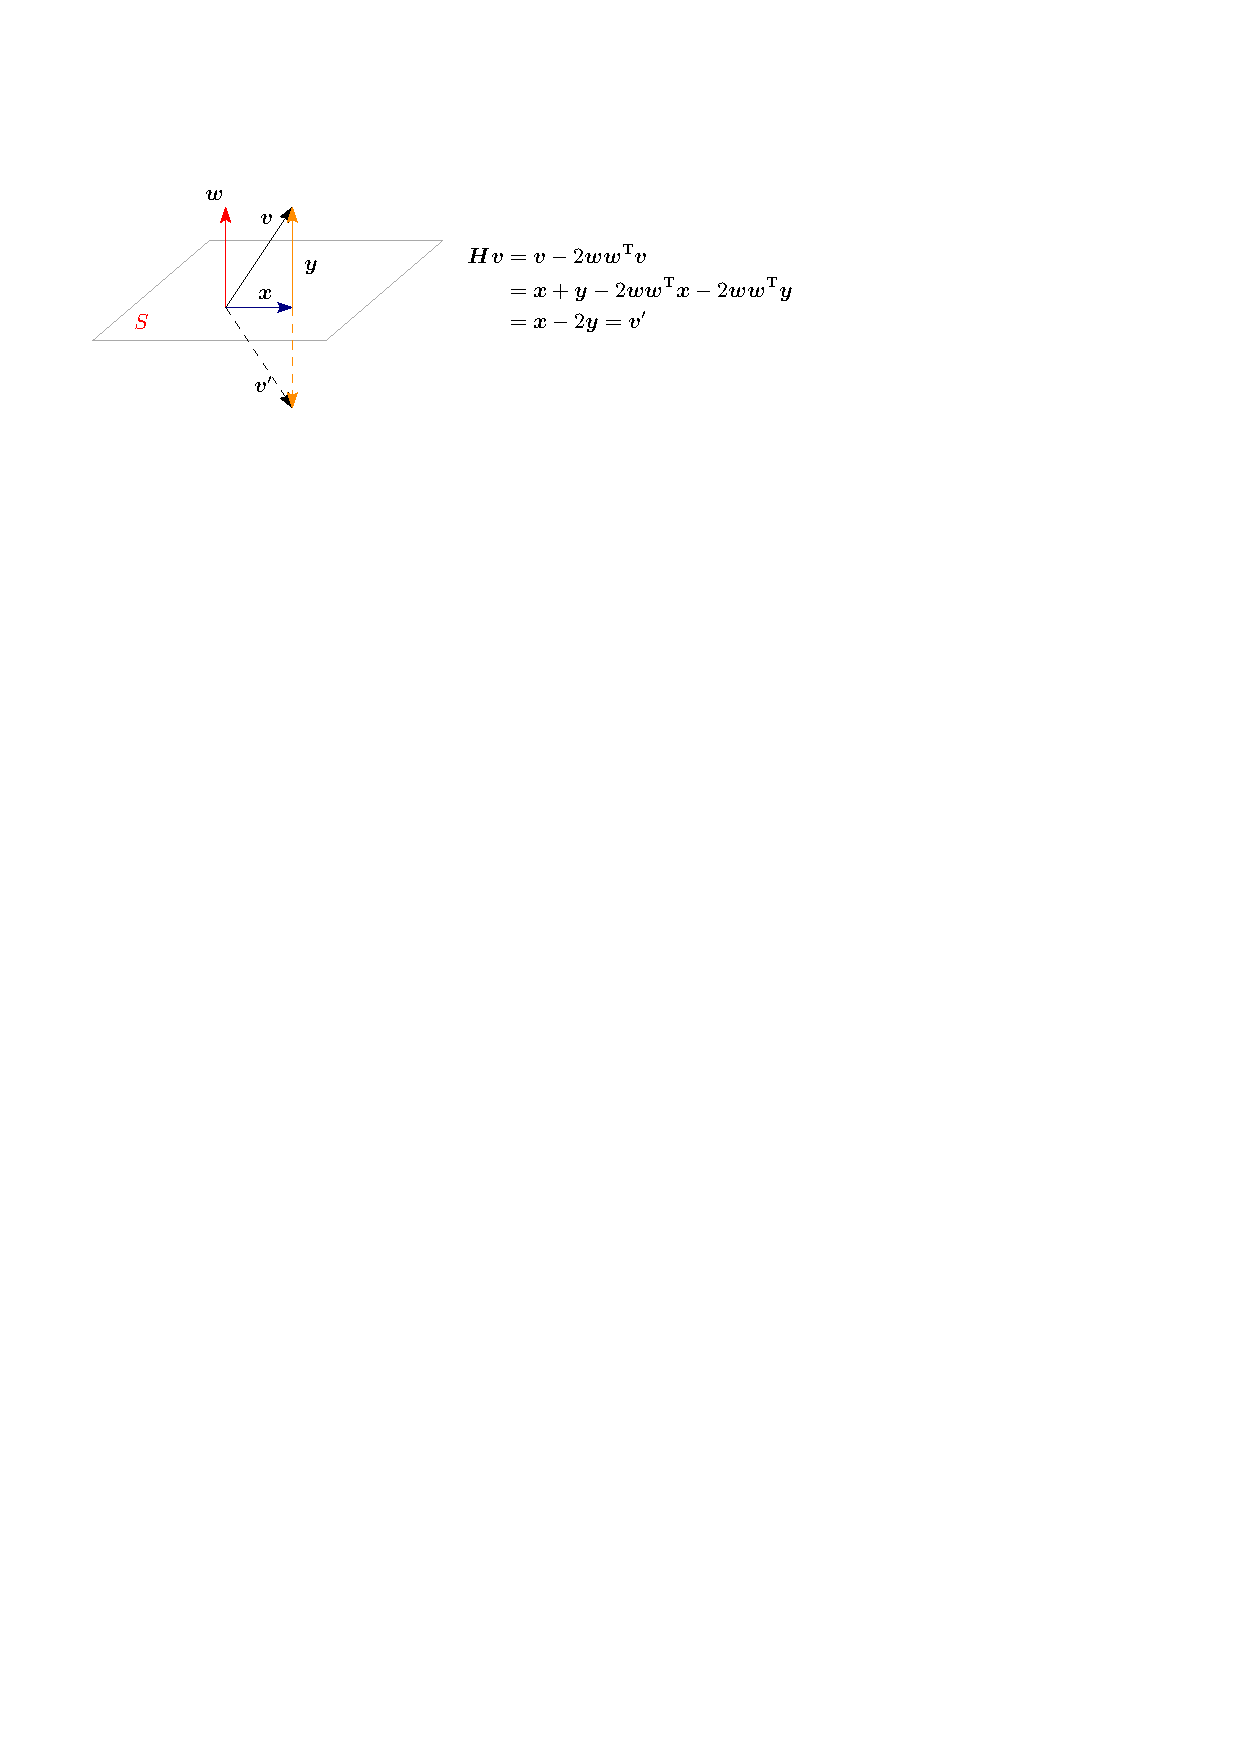
\includegraphics{image/Householder变换.pdf}
    \end{figure}
\end{note}
\subsection{Gauss消元法}
得到等价的线性代数方程组
\[
    \left\{
        \begin{aligned}
            a_{11}^{(1)}x_{1}+a_{12}^{(1)}x_{2}+\cdots+a_{1n}^{(1)}x_{n}=b_{1}^{(1)}\\
            a_{ii}^{(i)}x_{i}+a_{i,i+1}^{(i)}x_{i+1}+\cdots+a_{in}^{(i)}x_{n}=b_{i}^{(i)}\\
            \cdots\\
            a_{n-1,n-1}^{(n-1)}x_{n-1}+a_{n-1,n}^{(n-1)}x_{n}=b_{n-1}^{(n-1)}\\
            a_{nn}^{(n)}x_{n}=b_{n}^{(n)}
        \end{aligned} 
    \right.
\]
    
\begin{algorithm}[h]
    \SetAlgoLined
    \caption{Gauss消元法}
    \label{alg:Gauss}
    \KIN{$[\boldsymbol{A}\,| \boldsymbol{b}]$}
    \KOUT{$\boldsymbol{x}$}
    $\boldsymbol{Z} = [\boldsymbol{A}\,| \boldsymbol{b}]$\\
    \For{$k = 1\to n-1$}{
        \For{$i = k+1\to n$}{
            $\boldsymbol{Z}[i,:]\gets \boldsymbol{Z}[i,:]-\dfrac{a_{ik}^{(k)}}{a_{kk}^{(k)}}\boldsymbol{Z}[k,:]$
        }
    }
    $\boldsymbol{A} = \boldsymbol{Z}[:,1:n]$\\
    $\boldsymbol{b} = \boldsymbol{Z}[:,n+1]$\\
    \For{$i = n\to 1$}{
        $\boldsymbol{x}[{i}] = \boldsymbol{b}[i]$\\
        $\boldsymbol{x}[{i}] = \boldsymbol{x}[{i}]-\boldsymbol{A}[i,i+1:]\boldsymbol{x}[i+1:]$\\
        $\boldsymbol{x}[i] = \boldsymbol{x}[i]/\boldsymbol{A}[i,i]$
    }
    \Return {$\boldsymbol{x}$}
\end{algorithm}
\begin{note}
    高斯消元法的运算量
    \[
        MD = \dfrac{n^3}{3}-\dfrac{n}{3} = \dfrac{n^3}{3} + O(n)
    \]
\end{note}
\begin{example}
    用Gauss消去法解线性方程组(用四位有效数字计算)
    \[
        \left\{\begin{array}{c}0.0001x_1+2x_2=1\\2x_1+3x_2=2\end{array}\right.\boldsymbol{x}^*=\left(\begin{matrix}0.25001875\\0.49998750\end{matrix}\right)
    \]
    \begin{solution}
        用Gauss消去法求解
        \begin{figure}[h]
            \centering
            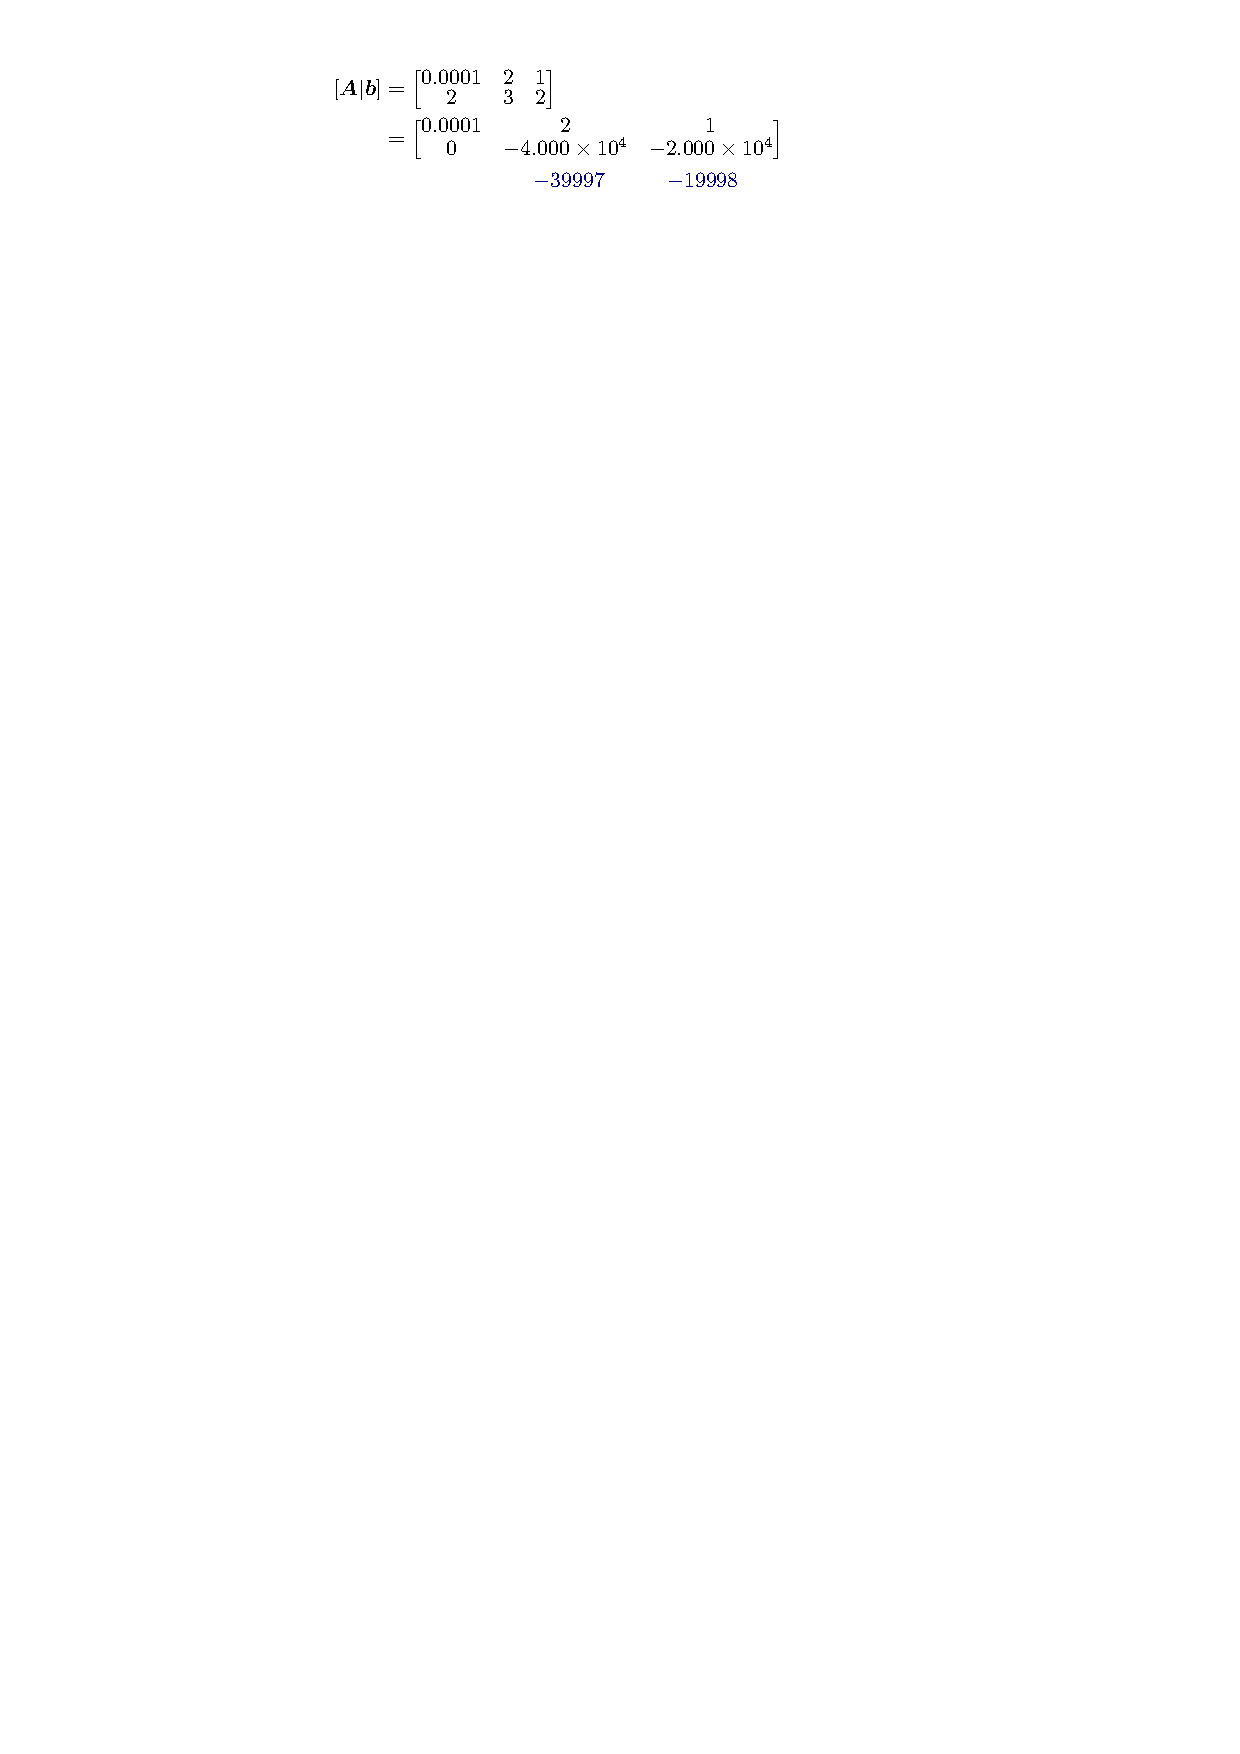
\includegraphics{image/Gauss-example1.pdf}
        \end{figure}
        回代得到$x_1 = 0.0000,\,x_2 = 0.5000$
    \end{solution}
\end{example}
\begin{note}
    问题:

    与精确解相比,该结果相当糟糕
    
    原因:在求行乘数时用了很小的数0.0001作除数
\end{note}
\begin{example}
    将两个方程互换为
    \[
        \left\{
            \begin{array}{rl}
                2x_1+3x_2=2\\
                0.0001x_1+2x_2=1
            \end{array}
        \right.
    \]
    \begin{solution}
        再采用Gauss消去法求解
        \begin{figure}[h]
            \centering
            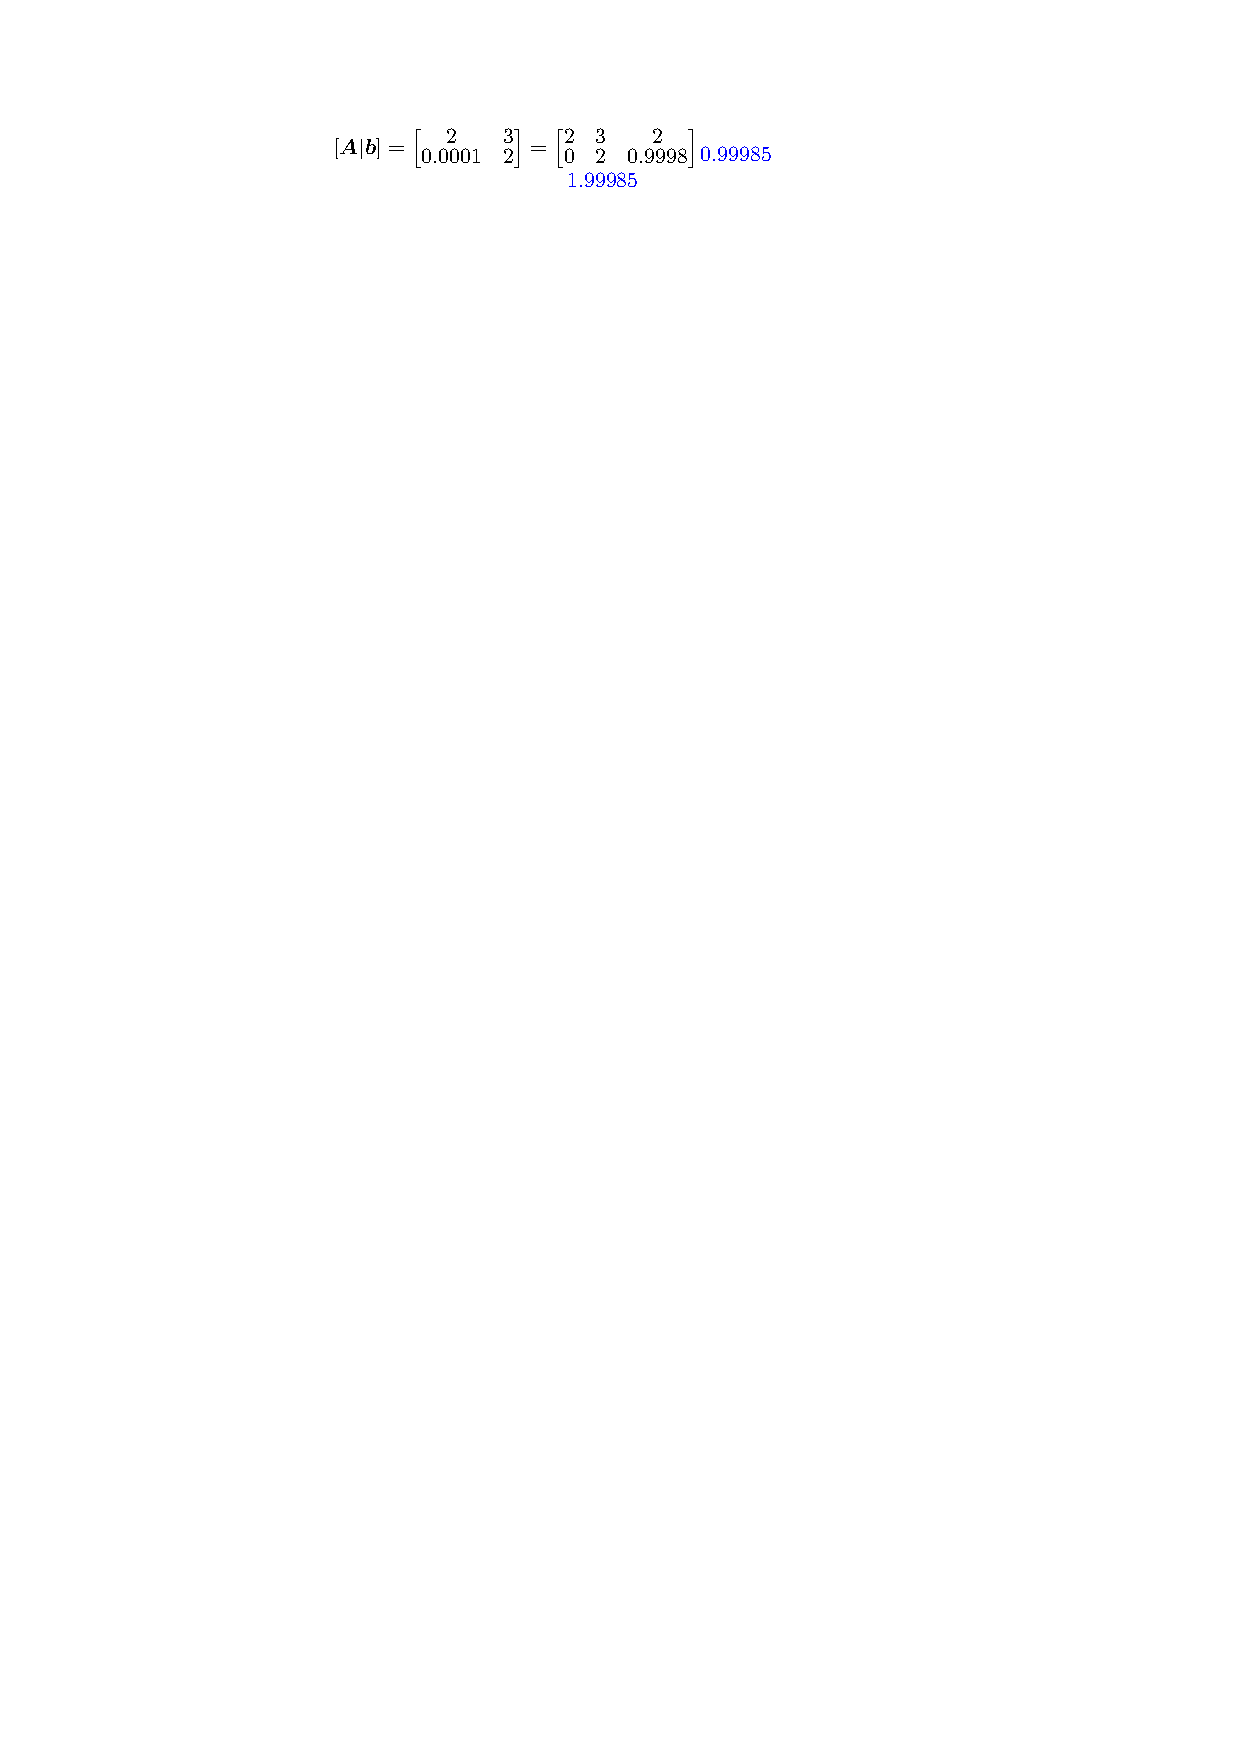
\includegraphics{image/Gauss-example2.pdf}
        \end{figure}
        回代得到$x_1 = 0.2500,\,x_2 = 0.5000$
    \end{solution}
\end{example}
\begin{definition}[列主元Gauss消元法]
    经过$k$步约化后
    \[
        \boldsymbol{A}\to \boldsymbol{A}^{(k)}=
        \begin{bmatrix}
            a_{11}^{(1)} & a_{12}^{(1)} & \cdots & & \cdots & a_{1n}^{(1)}\\
            & a_{22}^{(2)} & \cdots & & \cdots & a_{2n}^{(2)}\\
            & & \ddots & & & \\
            & & & a_{kk}^{(k)} & \cdots & a_{kn}^{(k)}\\
            & & & \vdots & & \\
            \multicolumn{3}{c}{\resizebox{4ex}{!}{$\boldsymbol{0}$}} & a_{mk}^{(k)} & \cdots & a_{mn}^{(k)}
        \end{bmatrix}
    \]
    在$\boldsymbol{A}^{(k)}$的第$k$列选主元,$\mid a_{i_k,k}^{(k)}\mid=\max_{k\leq i\leq n}\mid a_{ik}^{(k)}\mid$。若$i_k>k$,则在$[\boldsymbol{A}^{(k)}\mid \boldsymbol{b}^{(k)}]$中将$i_k$与$k$行互换,再按照Gauss消元公式求出$[A^{(k+1)}\mid b^{(k+1)}]$。重复以上过程直到求出$[\boldsymbol{A}^{(n)}|\boldsymbol{b}^{(n)}]$
\end{definition}
\begin{example}
    要将这段顺序Gauss消元法的Matlab程序改成列主元Gauss消元法,需要在\sol{A} 处添加代码\Stars{3}
    
    \begin{algorithm}[H]
        \SetAlgoLined
        \caption{Gauss列主元消元法}
        \label{alg:GaussElim}
        \KIN{$[\boldsymbol{A}\,| \boldsymbol{b}]$}
        \KOUT{$\boldsymbol{x}$}
        $\boldsymbol{Z} = [\boldsymbol{A}\,| \boldsymbol{b}]$\\
        \For{$k = 1\to n-1$}{
            \tcp*[l]{\colorbox{cyan!50}{A}}
            \For{$i = k+1\to n$}{
                \tcp*[l]{\colorbox{cyan!50}{B}}
                $\boldsymbol{Z}[i,:]\gets \boldsymbol{Z}[i,:]-\dfrac{a_{ik}^{(k)}}{a_{kk}^{(k)}}\boldsymbol{Z}[k,:]$
            }
            \tcp*[l]{\colorbox{cyan!50}{C}}
        }
        $\boldsymbol{A} = \boldsymbol{Z}[:,1:n]$\\
        $\boldsymbol{b} = \boldsymbol{Z}[:,n+1]$\\
        \For{$i = n\to 1$}{
            \tcp*[l]{\colorbox{cyan!50}{D}}
            $\boldsymbol{x}[{i}] = \boldsymbol{b}[i]$\\
            $\boldsymbol{x}[{i}] = \boldsymbol{x}[{i}]-\boldsymbol{A}[i,i+1:]\boldsymbol{x}[i+1:]$\\
            $\boldsymbol{x}[i] = \boldsymbol{x}[i]/\boldsymbol{A}[i,i]$
        }
        \Return {$\boldsymbol{x}$}
    \end{algorithm}
\end{example}
\subsection{直接三角分解法}
经过以下变换
\[
    \boldsymbol{L}_{1}\left(\boldsymbol{l}_{1}\right)= \boldsymbol{I}-\boldsymbol{l}_{1}\boldsymbol{e}_{1}^{\mathrm{T}}
\]
\[
    \boldsymbol{l}_1 = \begin{pmatrix}
        0&\frac{a_{21}}{a_{11}} &\frac{a_{31}}{a_{11}} &\frac{a_{41}}{a_{11}}
    \end{pmatrix}^{\mathrm{T}}
\]
\[
    \boldsymbol{L}_{1}\left(\boldsymbol{l}_{1}\right)=
    \begin{pmatrix}
        1& & &\\
        -\dfrac{a_{21}^{(1)}}{a_{11}^1}& 1 & & \\
        -\dfrac{a_{31}^{(1)}}{a_{11}^1}& & 1 & \\
        -\dfrac{a_{41}^{(1)}}{a_{11}^1}& & & 1 \\
    \end{pmatrix}
    ,\,
    \begin{bmatrix}
        \boldsymbol{A}^{(2)} & \boldsymbol{b}^{(2)}
    \end{bmatrix}  = \boldsymbol{L}_{1}\left(\boldsymbol{l}_{1}\right) 
    \begin{bmatrix}
        \boldsymbol{A}^{(1)} & \boldsymbol{b}^{(1)}
    \end{bmatrix}
\]
\[
    \boldsymbol{L}_{2}\left(\boldsymbol{l}_{2}\right)=
    \begin{pmatrix}
        1 & & &\\
        0 & 1 & & \\
        0 &-\dfrac{a_{32}^{(2)}}{a_{22}^{(2)}}&1&  \\
        0 &-\dfrac{a_{42}^{(2)}}{a_{22}^{(2)}}&&1 \\
    \end{pmatrix}
    ,\,
    \begin{bmatrix}
        \boldsymbol{A}^{(3)} & \boldsymbol{b}^{(3)}
    \end{bmatrix}  = \boldsymbol{L}_{2}\left(\boldsymbol{l}_{2}\right) 
    \begin{bmatrix}
        \boldsymbol{A}^{(2)} & \boldsymbol{b}^{(2)}
    \end{bmatrix}
\]
\[
    \boldsymbol{L'A} = \boldsymbol{U}\Rightarrow\boldsymbol{A} = \boldsymbol{LU}
\]
其中
\[
    \boldsymbol{L}'=\boldsymbol{L}_1(\boldsymbol{l}_2)\boldsymbol{L}_2(\boldsymbol{l}_1)\cdots \boldsymbol{L}_{n-1}(\boldsymbol{l}_{n-1})=\begin{bmatrix}1&&&&\\l_{21}&1&&&\\\vdots&l_{32}&\ddots&&\\\vdots&\vdots&&\ddots&\\l_{n1}&l_{n2}&\cdots&\cdots&1\end{bmatrix}
\]
\begin{theorem}
    设$\boldsymbol{A}\in \mathbb{R}^{n\times n}$非奇异,且各阶顺序主子式
    \[
        D_k=\det\:\boldsymbol{A}_k=
        \begin{vmatrix}
            a_{11}&\cdots&a_{1k}\\
            \vdots&&\vdots\\
            a_{k1}&\cdots&a_{kk}
        \end{vmatrix}\neq0
    \]
    则$\boldsymbol{A}$可唯一地分解为一个单 位下三角阵$\boldsymbol{L}$与一个上三角阵$\boldsymbol{U}$的乘积,即
    \[
        \boldsymbol{A} = \boldsymbol{LU}
    \]
\end{theorem}
\begin{example}
    请将下列矩阵进行三角分解\Stars{3}
    \[
        \boldsymbol{A} = 
        \begin{bmatrix}
            2   & -1  & 3 \\
            4   & 2   & 5 \\
            1   & 2   & 0 \\
        \end{bmatrix}
    \]
    \begin{solution}
        \begin{table}[H]
            \centering
            \begin{tabular}{cc|c|c|c|c|c|c|c|}
                \cline{3-5}\cline{7-9}    第一行 & $\boldsymbol{L}$ & 1   & 0   & 0   & $\boldsymbol{U}$ & \cellcolor[rgb]{ 1,  1,  0}2 & \cellcolor[rgb]{ 1,  1,  0}-1 & \cellcolor[rgb]{ 1,  1,  0}3 \bigstrut\\
                \cline{3-5}\cline{7-9}        &     &     & 1   & 0   &     & 0   &     &  \bigstrut\\
                \cline{3-5}\cline{7-9}        &     &     &     & 1   &     & 0   & 0   &  \bigstrut\\
                \cline{3-5}\cline{7-9}    
        \end{tabular}%
        \end{table}
        \begin{table}[H]
            \centering
            \begin{tabular}{cc|c|c|c|c|c|c|c|}
                \cline{3-5}\cline{7-9}    第一列 & $\boldsymbol{L}$ & 1   & 0   & 0   & $\boldsymbol{U}$ & 2   & -1  & 3 \bigstrut\\
                \cline{3-5}\cline{7-9}        &     & \cellcolor[rgb]{ 1,  1,  0}2 & 1   & 0   &     & 0   &     &  \bigstrut\\
                \cline{3-5}\cline{7-9}        &     & \cellcolor[rgb]{ 1,  1,  0}$\frac{1}{2}$ &     & 1   &     & 0   & 0   &  \bigstrut\\
                \cline{3-5}\cline{7-9}    
            \end{tabular}%
        \end{table}%
        \begin{table}[H]
            \centering
            \begin{tabular}{cc|c|c|c|c|c|c|c|}
                \cline{3-5}\cline{7-9}    第二行 & $\boldsymbol{L}$ & 1   & 0   & 0   & $\boldsymbol{U}$ & 2   & -1  & 3 \bigstrut\\
                \cline{3-5}\cline{7-9}        &     & 2   & 1   & 0   &     & 0   & \cellcolor[rgb]{ 1,  1,  0}4 & \cellcolor[rgb]{ 1,  1,  0}-1 \bigstrut\\
                \cline{3-5}\cline{7-9}        &     & $\frac{1}{2}$ &     & 1   &     & 0   & 0   &  \bigstrut\\
                \cline{3-5}\cline{7-9}    
            \end{tabular}%
        \end{table}%
        \begin{table}[H]
            \centering
            \begin{tabular}{cc|c|c|c|c|c|c|c|}
                \cline{3-5}\cline{7-9}    第二列 & $\boldsymbol{L}$ & 1   & 0   & 0   & $\boldsymbol{U}$ & 2   & -1  & 3 \bigstrut\\
                \cline{3-5}\cline{7-9}        &     & 2   & 1   & 0   &     & 0   & 4   & -1 \bigstrut\\
                \cline{3-5}\cline{7-9}        &     & $\frac{1}{2}$ & \cellcolor[rgb]{ 1,  1,  0}$\frac{5}{8}$ & 1   &     & 0   & 0   &  \bigstrut\\
                \cline{3-5}\cline{7-9}    
            \end{tabular}%
          \end{table}%
          \begin{table}[H]
            \centering
            \begin{tabular}{cc|c|c|c|c|c|c|c|}
                \cline{3-5}\cline{7-9}    第三行 & $\boldsymbol{L}$ & 1   & 0   & 0   & $\boldsymbol{U}$ & 2   & -1  & 3 \bigstrut\\
                \cline{3-5}\cline{7-9}        &     & 2   & 1   & 0   &     & 0   & 4   & -1 \bigstrut\\
                \cline{3-5}\cline{7-9}        &     & $\frac{1}{2}$ & $\frac{5}{8}$ & 1   &     & 0   & 0   & \cellcolor[rgb]{ 1,  1,  0}$-\frac{7}{8}$ \bigstrut\\
                \cline{3-5}\cline{7-9}    
            \end{tabular}%
        \end{table}%
    \end{solution}
\end{example}
\begin{example}
    用Doolittle分解法求解线性方程组\Stars{4}
    \[
        \begin{bmatrix}
            2 & 1 & 1\\
            1 & 3 & 2\\
            1 & 2 & 1\\
        \end{bmatrix}
        \begin{bmatrix}
            x_1\\x_2\\x_3
        \end{bmatrix}
         = \begin{bmatrix}
            4 \\ 6 \\ 5
         \end{bmatrix}
    \]
    \begin{solution}
        \[
            \boldsymbol{L} = \begin{bmatrix}
                1 &&\\
                1/2&1&\\
                1/2&3/5&1
            \end{bmatrix}
            ,\,
            \boldsymbol{U} = \begin{bmatrix}
                2 &1&1\\
                &5/2&3/2\\
                &&3/5
            \end{bmatrix}
        \]
        
        求解$\boldsymbol{Ly} = \boldsymbol{b}$得$\boldsymbol{y} = (4,4,3/5)^{\mathrm{T}}$

        求解$\boldsymbol{Ux} = \boldsymbol{y}$得$\boldsymbol{x} = (1,1,1)^{\mathrm{T}}$
    \end{solution}
\end{example}
\begin{definition}
    若$\boldsymbol{A}\in \mathbb{R}^{n\times n}$对称正定,则存在唯一的对角元为正的下三角矩阵$\boldsymbol{L}$,使$\boldsymbol{A}$分解为
    \[
        \boldsymbol{A} = \boldsymbol{L}\boldsymbol{L}^{\mathrm{T}}
    \]
\end{definition}
\begin{example}
    用平方根法求解线性方程组\Stars{4}
    \[
        \begin{pmatrix}
            4&-1&1\\
            -1&4.25&2.75\\
            1&2.75&3.5
        \end{pmatrix}
        \begin{pmatrix}
            x_1\\x_2\\x_3
        \end{pmatrix}=
        \begin{pmatrix}
            6\\-0.5\\1.25
        \end{pmatrix}
    \]
    则分解后矩阵中的$l_{21}=\sol{-0.5}$。
\end{example}
\subsection{大型带状方程组的求解}
\begin{definition}[三对角方程]
    方程组$\boldsymbol{Ax} = \boldsymbol{f}$称为三对角方程

    其中
    \[
        \boldsymbol{A}=\begin{bmatrix}
            b_1&c_1&&&\\
            a_2&b_2&c_2&&\\
            &a_3&b_3&\ddots&\\
            &&\ddots&\ddots&c_{n-1}\\
            &&&a_n&b_n
        \end{bmatrix},\quad 
        \boldsymbol{f}=\begin{bmatrix}
            f_1\\f_2\\f_3\\\vdots\\f_n
            \end{bmatrix}.
    \]
\end{definition}
\[
    \begin{aligned}
        &\boldsymbol{A}=
        \begin{pmatrix}
            b_1&c_1&&&\\
            a_2&b_2&c_2&&\\
            &\ddots&\ddots&\ddots&\\
            &&a_{n-1}&b_{n-1}&c_{n-1}\\
            &&&a_n&b_n
        \end{pmatrix}\\
        &=\begin{pmatrix}
            \alpha_1&\alpha_1\beta_1&&&\\
            \gamma_2&\gamma_2\beta_1+\alpha_2&\alpha_2\beta_2&&\\
            &\gamma_3&\ddots&\ddots&\\&&\ddots&\gamma_{n-1}\beta_{n-2}+\alpha_{n-1}&\alpha_{n-1}\beta_{n-1}\\
            &&&\gamma_n&\gamma_n\beta_{n-1}+\alpha_n
        \end{pmatrix}
    \end{aligned}
\]
\subsection{向量和矩阵范数}
\begin{definition}
    设$\boldsymbol{x}\in\mathbb{R}^n($或$\boldsymbol{x}\in\mathbb{C}^n)$,关于$\boldsymbol{x}$的某个实值非负函数$N(\boldsymbol{x})\equiv\parallel \boldsymbol{x}\parallel$,如果满足下列条件:
    \begin{enumerate}
        \item $\| \boldsymbol{x}\| \geq 0$,且$\|\boldsymbol{x}\|=0\Leftrightarrow \boldsymbol{x}=0$
        \item $\| \alpha \boldsymbol{x}\| = | \alpha \mid \cdot \| \boldsymbol{x}\| , \alpha \in \mathbb{R} ( \mathbb{C} ) ;$
        \item $\| \boldsymbol{x}+ y\| \leq \| \boldsymbol{x}\| + \| y\| , \forall \boldsymbol{x}, \boldsymbol{y}\in \mathbb{R} ^n( \mathbb{C}^n) .$
    \end{enumerate}
    则称$N(\boldsymbol{x})\equiv\parallel \boldsymbol{x}\parallel$是$\mathbb{R}^n($或$\boldsymbol{x}\in\mathbb{C}^n)$上的一个向量范数(或模)。
\end{definition}
\begin{note}
    常用的向量范数

    有$\boldsymbol{x} = \left( x_1,x_2,\cdots,x_n \right)^{\mathrm{T}}\in\mathbb{R}^n$
    
    \begin{itemize}
        \item $\infty$范数$\|\boldsymbol{x}\|_{\infty} = \max\limits_{1\leq i\leq n}|x_i|$
        \item 1-范数$\|\boldsymbol{x}\|_{1}  = \sum\limits_{i = 1}^{n}|x_i|$
        \item 2-范数$\|\boldsymbol{x}\|_{2}  = \sum\limits_{i = 1}^{n}\left( x_i^2 \right)^{1/2}$
    \end{itemize}
\end{note}
\begin{definition}[向量的$w$范数]
    向量的$w$范数由矩阵$\boldsymbol{w}$诱导
    \begin{enumerate}
        \item 设$N(\boldsymbol{x}) = \|\boldsymbol{x}\|_{v}$是$\mathbb{R}^{n}$上的一个向量范数
        \item 设$\boldsymbol{w}\in\mathbb{R}^{n\times n}$为非奇异矩阵,则$M(\boldsymbol{x})\equiv\|\boldsymbol{x}\|_{w}\equiv \|\boldsymbol{wx}\|_{v}$是$\mathbb{R}^n$上的一个向量范数
    \end{enumerate}
\end{definition}
\begin{definition}[矩阵范数]
    关于矩阵$\boldsymbol{A}\in\mathbb{R}^{n\times n}$的某个实值非负函数$N(\boldsymbol{A})\equiv\parallel \boldsymbol{A}\parallel$,如果满足下列条件:
    \begin{enumerate}
        \item $\parallel \boldsymbol{A}\parallel \geq 0$,且$\parallel \boldsymbol{A}\parallel=0\Leftrightarrow \boldsymbol{A}=0;$
        \item $\parallel \alpha \boldsymbol{A}\parallel = \mid \alpha \mid \cdot \parallel \boldsymbol{A}\parallel , \alpha \in \mathbb{R} ;$
        \item $\parallel \boldsymbol{A}+ \boldsymbol{B}\parallel \leq \parallel \boldsymbol{A}\parallel + \parallel \boldsymbol{B}\parallel , \forall \boldsymbol{A}, \boldsymbol{B}\in \mathbb{R} ^{n\times n};$
        \item $\parallel \boldsymbol{A}\boldsymbol{B}\parallel \leq \parallel \boldsymbol{A}\parallel \cdot \parallel \boldsymbol{B}\parallel , \forall \boldsymbol{A}, \boldsymbol{B}\in \mathbb{R} ^{m\times n}$。
    \end{enumerate}
则称$N(\boldsymbol{A})$是$\mathbb{R}^{n\times n}$上的一个矩阵范数(或模)。
\end{definition}
\begin{definition}[矩阵的F范数]
    $F(\boldsymbol{A})\equiv\|\boldsymbol{A}\|_{F} = \left( \sum\limits_{i,j = 1}^{n}a_{ij}^2 \right)^{1/2}$
\end{definition}
\begin{definition}[矩阵的算子范数]
    设$\boldsymbol{x}\in\mathbb{R}^n,\boldsymbol{A}\in\mathbb{R}^{n\times n}$,已经给出了一种向量范数$\|\boldsymbol{x}\|_{v}$定义一个矩阵的非负函数
    \[
        N(\boldsymbol{A})\equiv\parallel \boldsymbol{A}\parallel_{v}=\max_{\substack{\boldsymbol{x}\in\mathbb{R}^{n}\\\boldsymbol{x}\neq0}}\frac{\parallel \boldsymbol{A}\boldsymbol{x}\parallel_{v}}{\parallel \boldsymbol{x}\parallel_{v}}=\max_{\substack{y\in\mathbb{R}^{n}\\\parallel \boldsymbol{y}\parallel=1}}\parallel \boldsymbol{Ay}\parallel_{v}
    \]
\end{definition}
\begin{note}
    常用的矩阵范数
    
    设$\boldsymbol{x}\in\mathbb{R}^n,\boldsymbol{A}\in\mathbb{R}^{n\times n}$
    \begin{itemize}
        \item $\parallel \boldsymbol{A}\parallel_{\infty}=\max\limits_{1\leq i\leq n}\sum_{j=1}^{n}\mid a_{ij}\mid$,行范数
        \item $\parallel \boldsymbol{A}\parallel_1=\max\limits_{1\leq j\leq n}\sum_{i=1}^n\mid a_{ij}\mid$,列范数
        \item $\parallel \boldsymbol{A}\parallel_2=\sqrt{\rho(\boldsymbol{A}^\mathrm{T}\boldsymbol{A})}$,2-范数
    \end{itemize}
\end{note}
\begin{note}
    矩阵特征值的界
    \begin{enumerate}
        \item 设 $\boldsymbol{A}\in \mathbb{R} ^{n\times n}$,则$\rho(\boldsymbol{A})\leq\parallel \boldsymbol{A}\parallel_v$,
        $\left\|\boldsymbol{A}\right\|_v$为满足相容条件的矩阵范数;
        \item 设$\boldsymbol{A}\in\mathbb{R}^{n\times n}$为对称矩阵,则$\|\boldsymbol{A}\|_2=\rho(\boldsymbol{A})$
    \end{enumerate}
\end{note}
\begin{theorem}
    设$A\in\mathbb{R}^{n\times n},$则
    \[
        \operatorname*{lim}_{k\to\infty}\boldsymbol{A}^{k}=0\Leftrightarrow\rho(\boldsymbol{A})<1
    \]
\end{theorem}
\begin{theorem}
    设$\boldsymbol{B}\in\mathbb{R}^{n\times n}$,且$\parallel \boldsymbol{B}\parallel<1(\parallel \boldsymbol{B}\parallel$为矩阵的算子范数),则 $\boldsymbol{I}\pm \boldsymbol{B}$为非奇异矩阵,且有估计
    \[
        \|(\boldsymbol{I}\pm \boldsymbol{B})^{-1}\|\leq\frac{1}{1-\|\boldsymbol{B}\|}
    \]
\end{theorem}
\begin{proof}
    只证明$\boldsymbol{I}\pm \boldsymbol{B}$为非奇异矩阵,设$\boldsymbol{I}-\boldsymbol{B}$为奇异矩阵,则存在非零向量$\boldsymbol{x}$使得
    \[
        (\boldsymbol{I}+\boldsymbol{B})\boldsymbol{x} = \boldsymbol{0}
    \]
    那么有
    \[
        \begin{aligned}
            \|(\boldsymbol{I}+\boldsymbol{B})\boldsymbol{x}\|&= \|\boldsymbol{x}+\boldsymbol{B}\boldsymbol{x}\|\leq \|\boldsymbol{x}\| + \|\boldsymbol{B}\boldsymbol{x}\|\\
            &\leq \|\boldsymbol{x}\| + \|\boldsymbol{B}\|\|\boldsymbol{x}\| =(1+\|\boldsymbol{B}\|)\|\boldsymbol{x}\|\\
            &<2\|\boldsymbol{x}\|
        \end{aligned}
    \]
\end{proof}
\subsection{条件数与病态矩阵}
\begin{example}
    已知 $A=\begin{pmatrix}1&-3\\-1&2\end{pmatrix}$, 求$\left\|\boldsymbol{A}\right\|_\infty\left\|\boldsymbol{A}\right\|_1,\left\|\boldsymbol{A}\right\|_2.$\Stars{4}
    \begin{solution}
        $\| \boldsymbol{A}\|_{\infty }= 4\| \boldsymbol{A}\|_1= 5$
        \[
            \boldsymbol{A}^\mathrm{T}\boldsymbol{A}=
                \begin{pmatrix}1&-1\\-3&2\end{pmatrix}
                \begin{pmatrix}1&-3\\-1&2\end{pmatrix}
                =\begin{pmatrix}2&-5\\-5&13\end{pmatrix}
        \]
        \[
            \lambda_{1,2}=\frac{15\pm\sqrt{221}}2\quad
            \|\boldsymbol{A}\|_2=\sqrt{\frac{15+\sqrt{221}}2}\approx3.864
        \]
    \end{solution}
\end{example}
\begin{note}
    常用条件数:
    \[
        \mathrm{Cond}(\boldsymbol{A})_{\infty}= \|\boldsymbol{A}^{-1}\|_{\infty}\cdot \| \boldsymbol{A}\|_{\infty}
    \]

    \[
        \begin{aligned}
            &\mathrm{Cond}(\boldsymbol{A})_{2}= \| \boldsymbol{A}^{- 1}\|_{2}\cdot \| \boldsymbol{A}\| _{2} \\
            &= \sqrt{\lambda_{\max}\left(\boldsymbol{A}^{\mathrm{T}}\boldsymbol{A}\right)^{-1}}\cdot\sqrt{\lambda_{\max}\left(\boldsymbol{A}^{\mathrm{T}}\boldsymbol{A}\right)}=\frac{\sqrt{\lambda_{\max}\left(\boldsymbol{A}^{\mathrm{T}}\boldsymbol{A}\right)}}{\sqrt{\lambda_{\min}\left(\boldsymbol{A}^{\mathrm{T}}\boldsymbol{A}\right)}}
        \end{aligned}
    \]
    $\boldsymbol{A}$非奇异、对称,$\|\lambda_1\|\geq\|\lambda_2\|\geq\cdots\geq\|\lambda_n\|$
    \[
        \mathrm{Cond}(\boldsymbol{A})_2=\frac{\|\lambda_1\|}{\|\lambda_n\|}
    \]
\end{note}
\begin{example}
    $\boldsymbol{A}=\begin{bmatrix}1.&1.\\1.&1.0001\end{bmatrix}$的条件数$\operatorname{Cond}(\boldsymbol{A})_{\infty}=$\sol{40000}
    \begin{solution}
        \[
            \boldsymbol{A}=\begin{bmatrix}1.&1.\\1.&1.0001\end{bmatrix}
        \]
        \[
            \boldsymbol{A}^{-1}=\begin{bmatrix}1.0001&-1.\\-1.&1.\end{bmatrix}\cdotp\frac1{0.0001}
        \]
        \[
            \| \boldsymbol{A}\|_\infty=2.0001\quad\| \boldsymbol{A}^{-1}\|_\infty=2.0001\times10^4
        \]
        \[
            \operatorname{Cond}(\boldsymbol{A})_\infty\approx4.\times10^4
        \]
    \end{solution}
\end{example}
\begin{note}
    如何判断$\boldsymbol{Ax} = \boldsymbol{b}$是病态?
    \begin{enumerate}
        \item 估计条件数;
        \item 若用列主元消去法求解方程组$\boldsymbol{Ax} = \boldsymbol{b}$,在约化中出现小主元,可能是病态;
        \item $\boldsymbol{Ax} = \boldsymbol{b}$出现一个相对很大的解,可能是病态;
        \item $\boldsymbol{A}$中的元素的数量级相差很大,可能是病态;
        \item 当$\det(\boldsymbol{A})$相对很小、或$\boldsymbol{A}$某些行(列)近似线性相关,可能是病态
    \end{enumerate}
\end{note}
\section{解线性方程组的迭代法}
\subsection{迭代法的构造}
\begin{note}
    迭代法的基本思想:

    \[
        \boldsymbol{Ax}=\boldsymbol{b}\Leftrightarrow \boldsymbol{x}=\boldsymbol{Bx}+\boldsymbol{f}
    \]
    选取初始向量$x^{(0)}$,构造迭代格式:
    \[
        \begin{aligned}
            \boldsymbol{x}^{(1)} = \boldsymbol{Bx}^{(0)}+\boldsymbol{f}\\
            \boldsymbol{x}^{(2)} = \boldsymbol{Bx}^{(1)}+\boldsymbol{f}\\
            \vdots\\
            \boldsymbol{x}^{(k)} = \boldsymbol{Bx}^{(k-1)}+\boldsymbol{f}\\
        \end{aligned}
    \]
    两边取极限得到
    \[
        \boldsymbol{x}^* = \boldsymbol{Bx}^*+\boldsymbol{f}
    \]
\end{note}
\begin{note}
    迭代法构造的一般原则:

    将系数矩阵分解为
    \[
        \boldsymbol{A} = \boldsymbol{M}-\boldsymbol{N}
    \]
    故而有
    \[
        \boldsymbol{Ax}=\boldsymbol{b}\Leftrightarrow \boldsymbol{Mx}=\boldsymbol{Nx}+\boldsymbol{b}
    \]
    从而方程组等价化为
    \[
        \boldsymbol{x} =\boldsymbol{M}^{-1}\boldsymbol{Nx}+\boldsymbol{M}^{-1}\boldsymbol{b}
    \]
    需要满足以下条件
    \begin{itemize}
        \item $\boldsymbol{M}$非奇异
        \item $\boldsymbol{M}^{-1}$容易求
    \end{itemize}
\end{note}
迭代法的收敛性

\begin{theorem}[迭代法基本定理]
    对于任意的初始向量$\boldsymbol{x}^{(0)}$,迭代法构
    \[
        \boldsymbol{x}^{(k)} = \boldsymbol{Bx}^{(k-1)}+\boldsymbol{f}
    \]
    收敛的充分必要条件为
    \[
        |\lambda_{i}(\boldsymbol{B})|<1,\quad (i = 1,\cdots,n)
    \]
    或者
    \[
        \rho(\boldsymbol{B})<1
    \]
\end{theorem}
\begin{example}
    用迭代法求解下列方程组
    \[
        \begin{cases}
            8x_1-3x_2+2x_3=20\\
            4x_1+11x_2-x_3=33\\
            6x_1+3x_2+12x_3=36
        \end{cases}
        \quad
        \begin{pmatrix}x_1\\x_2\\x_3\end{pmatrix}
        =
        \begin{pmatrix}3.0000\\2.0000\\1.0000\end{pmatrix}
    \]
    \begin{solution}
        将系数矩阵分解为
        \[
            \begin{pmatrix}
                8 & -3 & 2\\
                4 & 11 & -1\\
                6 & 3 & 12
            \end{pmatrix} = 
            \begin{pmatrix}
                8 &  & \\
                 & 11 & \\
                 &  & 12
            \end{pmatrix}-
            \begin{pmatrix}
                0 & 3 & -2\\
                -4 & 0 & 1\\
                -6 & -3 & 0
            \end{pmatrix}
        \]
        从而构造迭代法
        \[
            \boldsymbol{x}^{k} = 
                \boldsymbol{M}^{-1}\boldsymbol{N}\boldsymbol{x}^{(k-1)}+\boldsymbol{M}^{-1}\boldsymbol{b}
        \]
    \end{solution}
\end{example}
\begin{theorem}
    对于任意的初始向量$\boldsymbol{x}^{(0)}$,若存在$\boldsymbol{B}$的某种范数$\parallel\cdot\parallel$,使得$\parallel \boldsymbol{B}\parallel=q<1$,则迭代法收敛,且
    \begin{enumerate}
        \item $\parallel \boldsymbol{x}^{(k)}-\boldsymbol{x}^{*}\parallel\leq\frac{q}{1-q}\parallel \boldsymbol{x}^{(k)}-\boldsymbol{x}^{(k-1)}\parallel;$
        \item $\parallel \boldsymbol{x}^{(k)}-\boldsymbol{x}^{*}\parallel\leq\frac{q^{k}}{1-q}\parallel \boldsymbol{x}^{(1)}-\boldsymbol{x}^{(0)}\parallel.$
    \end{enumerate}
\end{theorem}
\begin{proof}
    先证明1
    \[
        \begin{aligned}
            \parallel \boldsymbol{x}^{(k)}-\boldsymbol{x}^{*}\parallel&= \|\boldsymbol{B}(\boldsymbol{x}^{(k-1)}-\boldsymbol{x}^{*})\|\\
            &\leq \|\boldsymbol{B}\|\|(\boldsymbol{x}^{(k-1)}-\boldsymbol{x}^{*})\|\\
            & = \|\boldsymbol{B}\|\|(\boldsymbol{x}^{(k-1)}-\boldsymbol{x}^{k}) + (\boldsymbol{x}^{(k)}-\boldsymbol{x}^{*})\|\\
            & \leq \|\boldsymbol{B}\|\|(\boldsymbol{x}^{(k)}-\boldsymbol{x}^{(k-1)}) \| + \|\boldsymbol{B}\|\| (\boldsymbol{x}^{(k)}-\boldsymbol{x}^{*})\|\\
            & = q\|\boldsymbol{x}^{(k)}-\boldsymbol{x}^{(k-1)} \| + q\| \boldsymbol{x}^{(k)}-\boldsymbol{x}^{*}\|\\
        \end{aligned}  
    \]
    故而
    \[
        \parallel \boldsymbol{x}^{(k)}-\boldsymbol{x}^{*}\parallel\leq\frac{q}{1-q}\parallel \boldsymbol{x}^{(k)}-\boldsymbol{x}^{(k-1)}\parallel 
    \]

    再证明2
    \[
        \begin{aligned}
            \parallel \boldsymbol{x}^{(k)}-\boldsymbol{x}^{*}\parallel&\leq\frac{q}{1-q}\parallel \boldsymbol{x}^{(k)}-\boldsymbol{x}^{(k-1)}\parallel\\
            &\leq \frac{q^k}{1-q}\parallel \boldsymbol{x}^{(1)}-\boldsymbol{x}^{(0)}\parallel
        \end{aligned}
    \]
\end{proof}
\begin{example}
    对线性方程组
    \[
        \begin{pmatrix}3&2\\1&2\end{pmatrix}\begin{pmatrix}x_1\\x_2\end{pmatrix}=\begin{pmatrix}3\\-1\end{pmatrix}
    \]
    若用迭代法
    \[
        \boldsymbol{x}^{(k+1)}=\boldsymbol{x}^{(k)}+\alpha(\boldsymbol{A}\boldsymbol{x}^{(k)}-\boldsymbol{b})
    \]
    求解,则$\alpha\in$\sol{(-0.5,0)}时迭代收敛,$\alpha=$\sol{-0.4} 时迭代收敛最快。
    \begin{solution}
        由$\boldsymbol{x}^{(k+1)}=\boldsymbol{x}^{(k)}+\alpha(\boldsymbol{A}\boldsymbol{x}^{(k)}-b)$知道
        \[
            \boldsymbol{x}^{(k+1)}=(\alpha \boldsymbol{A}+\boldsymbol{I})\boldsymbol{x}^{(k)}-\alpha b
        \]
        求$\alpha \boldsymbol{A}+I$的谱半径$\rho$
        \[
            \begin{aligned}
                &\begin{vmatrix}
                    \lambda-3\alpha-1 & -2\alpha\\
                    -\alpha & \lambda-2\alpha-1
                \end{vmatrix}\\
                &=\lambda^2-(5\alpha+2)\lambda+(3\alpha+1)(2\alpha+1)-2\alpha^2\\
                &=\lambda^2-(5\alpha+2)\lambda+4\alpha^2+5\alpha+1\\
                &=[\lambda-(4\alpha+1)][\lambda-(\alpha+1)]
            \end{aligned}
        \]
        谱半径的图像$\rho = \max\left\{ |4\alpha+1|,|\alpha+1| \right\}$
        \begin{figure}[ht]
            \centering
            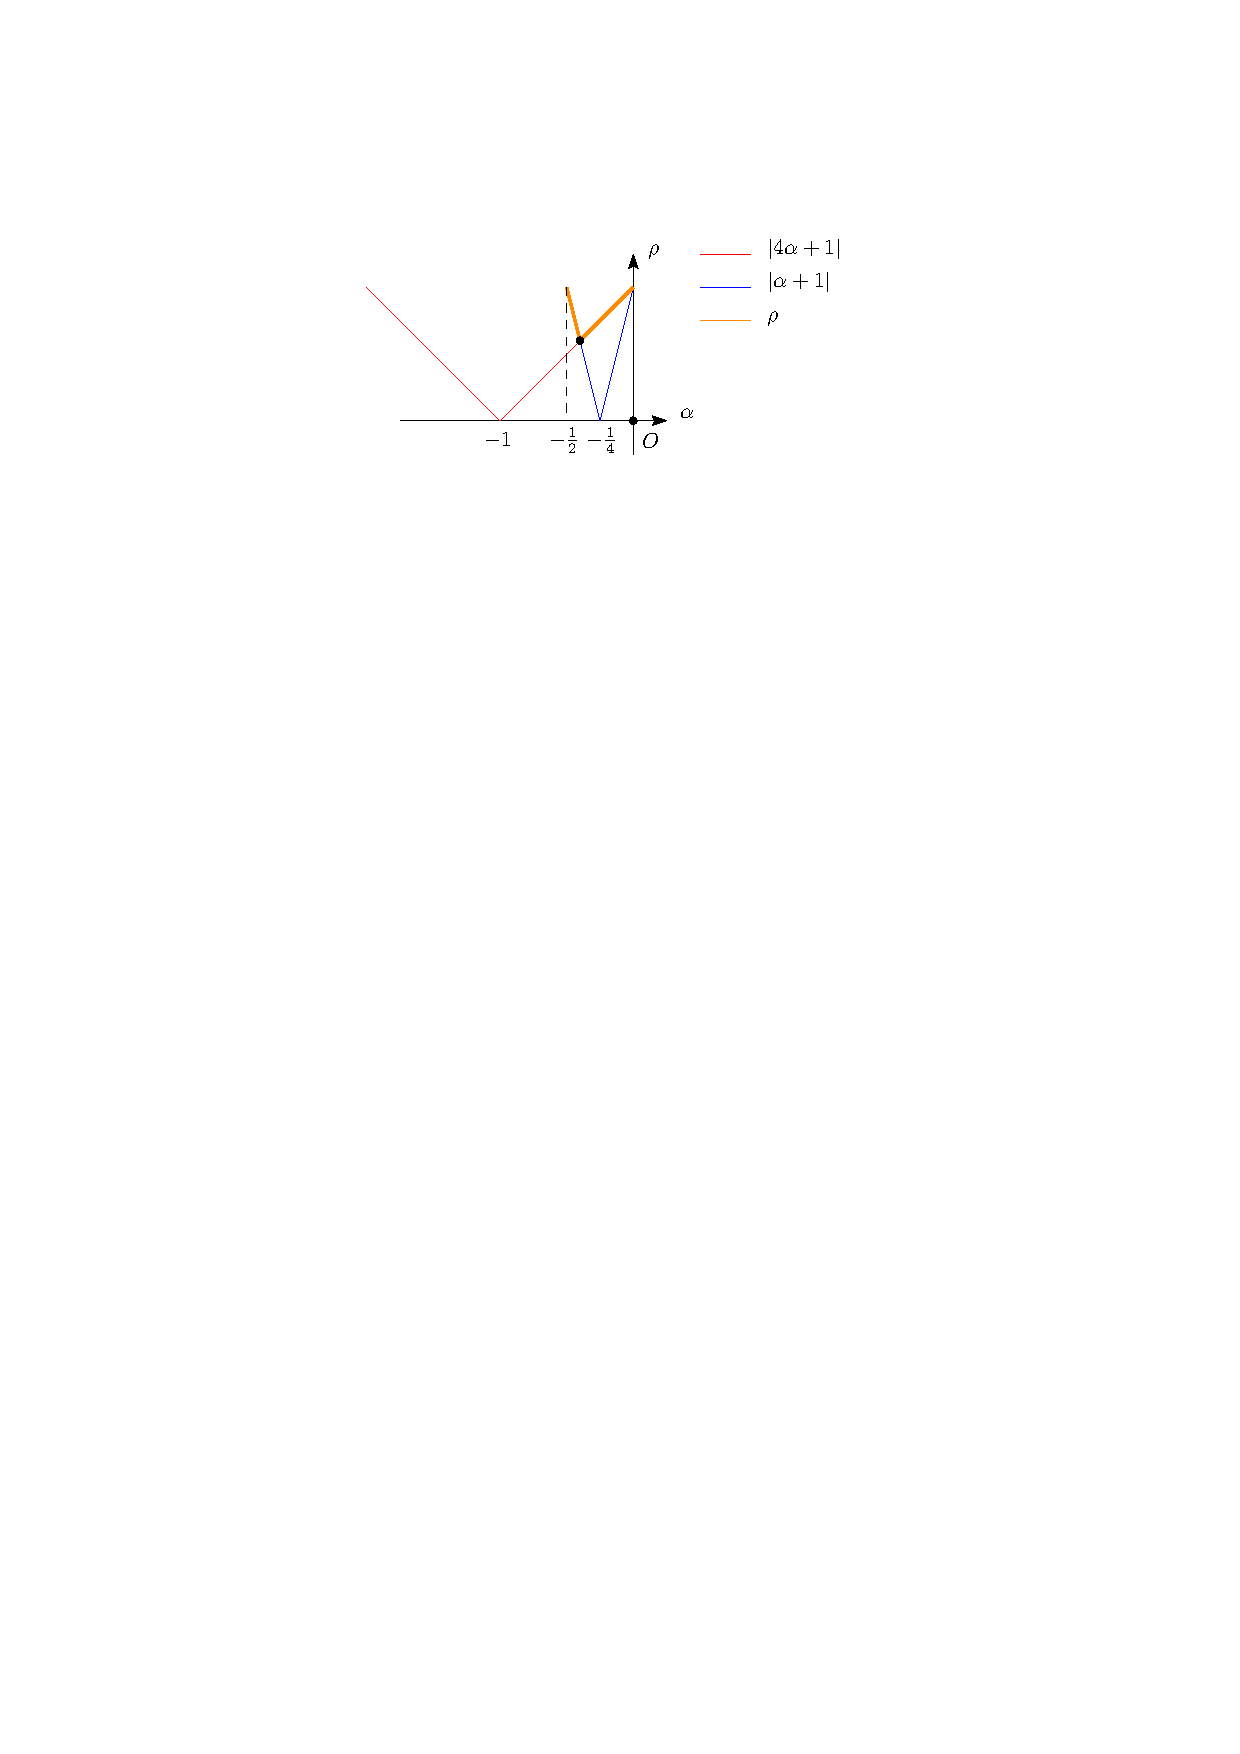
\includegraphics{image/迭代法rho-example.pdf}
        \end{figure}

        当$\alpha\in(-0.5,0)$时迭代收敛,$\alpha=-0.4$ 时迭代收敛最快
    \end{solution}
\end{example}
\subsubsection{Jacobi迭代法}
设$a_{ii}\neq 0,\,(i = 1,2,\cdots n),\,\boldsymbol{M} = \boldsymbol{D},\,\boldsymbol{N} = \boldsymbol{D}-\boldsymbol{A}$,有
\[
    \begin{array}{l}
        \boldsymbol{B}_{J} = \boldsymbol{D}^{-1}(\boldsymbol{D}-\boldsymbol{A}) = \boldsymbol{I}-\boldsymbol{D}^{-1}\boldsymbol{A} = \boldsymbol{D}^{-1}(\boldsymbol{L}+\boldsymbol{U})\\
        \boldsymbol{f} = \boldsymbol{D}^{-1}\boldsymbol{b}
    \end{array}
\]
\[
    \boldsymbol{x}^{(k+1)} = \boldsymbol{B}_{J}\boldsymbol{x}^{(k)}+\boldsymbol{f}
\]
\begin{theorem}[Jacobi迭代的收敛性定理]
    Jacobi迭代法收敛有以下结论
    \begin{itemize}
        \item Jacobi迭代法收敛的充分必要条件是
        \[
            \rho(\boldsymbol{B}_{J})<1        
        \]
        \item Jacobi迭代法收敛的充分条件是存在一种范数$\|\cdot\|$,使得$\|\boldsymbol{B}_{J}\|\leqslant 1$
    \end{itemize}
\end{theorem}
\subsubsection{Gauss-Seidel迭代法}
\[
    \begin{gathered}
        x_{1}^{(k+1)}=\frac{1}{a_{11}}(b_{1}-\sum_{j=2}^{n}a_{1j}x_{j}^{(k)}) \\
        \begin{aligned}x_{2}^{(k+1)}&=\frac{1}{a_{22}}(b_{2}-a_{21}x_{1}^{(k+1)}-\sum_{j=3}^{n}a_{2j}x_{j}^{(k)})\\&\cdots\cdots\end{aligned} \\
        x_{i}^{(k+1)}=\frac{1}{a_{ii}}(b_{i}-\sum_{j=1}^{i-1}a_{ij}x_{j}^{(k+1)}-\sum_{j=i+1}^{n}a_{ij}x_{j}^{(k)}) 
    \end{gathered}
\]
\[
    \boldsymbol{x}^{(k+1)} = \boldsymbol{G}\boldsymbol{x}^{(k)}+\boldsymbol{f}_{G}
\]
其中
\[
    \boldsymbol{G} = (\boldsymbol{D}-\boldsymbol{L})^{-1}\boldsymbol{U},\,\boldsymbol{f}_{G} = (\boldsymbol{D}-\boldsymbol{L})^{-1}\boldsymbol{b}
\]
\begin{theorem}[GS迭代的收敛性定理]
    GS迭代法收敛的充分必要条件是
    \begin{itemize}
        \item GS迭代法收敛的充分必要条件是
        \[
            \rho(\boldsymbol{G})<1        
        \]
        \item GS迭代法收敛的充分条件是存在一种范数$\|\cdot\|$,使得$\|\boldsymbol{G}\|\leqslant 1$
    \end{itemize}
\end{theorem}
\subsubsection{SOR}
\[
    \widetilde{x_i}^{(k+1)}=\frac1{a_{ii}}(b_i-\sum_{j=1}^{i-1}a_{ij}x_j^{(k+1)}-\sum_{j=i+1}^na_{ij}x_j^{(k)})
\]
\[
    \begin{aligned}
        x_{i}^{(k+1)}&=(1-\omega)x_{i}^{(k)}+\omega\widetilde{x}_{i}^{(k+1)}\\
        &=x_{i}^{(k)}+\omega\left(\widetilde{x}_{i}^{(k+1)}-x_{i}^{(k)}\right)\\
        &=(1-\omega)x_{i}^{(k)}+\frac{\omega}{a_{ii}}(b_{i}-\sum_{j=1}^{i-1}a_{ij}x_{j}^{^{(k+1)}}-\sum_{j=i+1}^{n}a_{ij}x_{j}^{^{(k)}})
    \end{aligned}
\]
其中$\omega$为可选择的松弛因子
\[
    \begin{array}{l}
        \boldsymbol{x}^{(k+1)} = (1-\omega)\boldsymbol{x}^{(k)}+\omega \boldsymbol{D}^{-1}\left( \boldsymbol{b}+\boldsymbol{L}\boldsymbol{x}^{(k+1)}+\boldsymbol{U}\boldsymbol{x}^{(k)} \right)\\
        (\boldsymbol{D}-\omega \boldsymbol{L})\boldsymbol{x}^{(k+1)} = [(1-\omega)\boldsymbol{D}+\omega \boldsymbol{U}]\boldsymbol{x}^{(k)} + \omega \boldsymbol{b}
    \end{array}
\]
表示为矩阵
\[
    \boldsymbol{x}^{(k+1)}=\boldsymbol{G}_\omega \boldsymbol{x}^{(k)}+\boldsymbol{f}_\omega 
\]
\[
    \boldsymbol{G}_\omega=(\boldsymbol{D}-\omega \boldsymbol{L})^{-1}[(1-\omega)\boldsymbol{D}+\omega \boldsymbol{U}]
\]
\[
    \boldsymbol{f}=\omega(\boldsymbol{D}-\omega \boldsymbol{L})^{-1}\boldsymbol{b}
\]
\begin{theorem}[(SOR方法收敛的必要条件)]
设解$\boldsymbol{Ax}=\boldsymbol{b}(\boldsymbol{A}\in\mathbb{R}^{n\times n})$的SOR方法收敛。则$0<\omega<2.$
\end{theorem}
\begin{proof}
    SOR法收敛就是$\rho(\boldsymbol{G}_\omega) <1$
    因为$\boldsymbol{G}_\omega = (D-\omega\boldsymbol{L})^{-1}[(1-\omega)\boldsymbol{D}+\omega\boldsymbol{U}]$
    \[
        |\det(\boldsymbol{D}-\omega \boldsymbol{L})| = \prod_{i = 1}^{n}|a_{ii}|
    \]
    \[
        |\det((1-\omega)\boldsymbol{D}+\omega \boldsymbol{U})| = |(1-\omega)^n|\prod_{i = 1}^{n}|a_{ii}|
    \]
    \[
        |\det (\boldsymbol{G}_{\omega})| = |(1-\omega)^n|\leq \rho(\boldsymbol{G}_{\omega})^{n}
    \]
    \[
        \begin{array}{l}
            |(1-\omega)|< \rho(\boldsymbol{G}_{\omega})<1\\
            -1<1-\omega<1\\
            0<\omega<2
        \end{array}
    \]
    证毕!
\end{proof}
\begin{note}
    关于解特殊方程组迭代法的收敛性
    \begin{definition}[对角占优]
        设$\boldsymbol{A}=(a_ij)\in\mathbb{R}^{n\times n}$,则
        \begin{itemize}
            \item 若$\mid a_{ii}\mid>\sum_{j=1}^{n}\mid a_{ij}\mid(i=1,2,\cdots,n)$,称$\boldsymbol{A}$为严格对角占优矩阵(或强占优阵)。
            \item 若$\mid a_ii\mid \geq \sum _{i= 1}^{n}\mid a_{ij}\mid ( j= 1, 2, \cdots , n)$, 且至少有一个不等式严格成立,则称$\boldsymbol{A}$为弱对角占优阵。
        \end{itemize}
    \end{definition}
    \begin{definition}[(可约与不可约阵)]
        设$\boldsymbol{A}=(a_{ij})\in\mathbb{R}^{n\times n}(n\geq2)$,如果存在置换矩阵 $\boldsymbol{P}$使
        \[
            \boldsymbol{P}^{\mathrm{T}}\boldsymbol{A}\boldsymbol{P}=\begin{pmatrix}\boldsymbol{A}_{11}&\boldsymbol{A}_{12}\\0&\boldsymbol{A}_{22}\end{pmatrix}
        \]
        其中$\boldsymbol{A}_{11}$为$r$阶方阵,$\boldsymbol{A}_{22}$为$n-r$阶方阵$(1\leq r<n)$,则称$\boldsymbol{A}$为可约矩阵;否则如果不存在这样的置换矩阵$\boldsymbol{P}$使上式成立,称$\boldsymbol{A}$为不可约阵.
    \end{definition}
    \[
        \boldsymbol{Ax} = \boldsymbol{b}\Rightarrow \boldsymbol{P}^{\mathrm{T}}\boldsymbol{A}\boldsymbol{P}\boldsymbol{P}^{\mathrm{T}}x = \boldsymbol{P}^{\mathrm{T}}\boldsymbol{b}
    \]
    \[
        \begin{pmatrix}\boldsymbol{A}_{11}&\boldsymbol{A}_{12}\\0&\boldsymbol{A}_{22}\end{pmatrix}\begin{pmatrix}
            y_1\\y_2
        \end{pmatrix} = \begin{pmatrix}
            \boldsymbol{C}_1\\\boldsymbol{C}_2
        \end{pmatrix}
    \]
\end{note}
\begin{theorem}
    设$\boldsymbol{Ax}=\boldsymbol{b}$,$\boldsymbol{A}=(a_{ij})\in\mathbb{R}^{n\times n}$,
    \begin{itemize}
        \item 如果$\boldsymbol{A}$为严格对角占优阵,则解方程组$\boldsymbol{Ax}=\boldsymbol{b}$的J法及GS法均收敛.
        \item 如果$\boldsymbol{A}$为弱对角占优阵且不可约阵,则解方程组 $\boldsymbol{Ax}=\boldsymbol{b}$的J法及GS法均收敛.
    \end{itemize}
\end{theorem}
\begin{theorem}
    设$\boldsymbol{A}=(a_{ij})\in\mathbb{R}^{n\times n}$,若
    \begin{enumerate}
        \item $\boldsymbol{A}$严格对角占优或弱对角占优且不可约,
        \item $0<\omega\leq1$,
    \end{enumerate}
    则解方程组$\boldsymbol{Ax}=\boldsymbol{b}$的SOR法收敛。
\end{theorem}
\begin{theorem}
    设$\boldsymbol{A}=(a_{ij})\in\mathbb{R}^{n\times n}$,若
    \begin{enumerate}
        \item $\boldsymbol{A}$为对称正定矩阵,
        \item $0< \omega < 2$,
    \end{enumerate}
    则解方程组$\boldsymbol{Ax}=\boldsymbol{b}$的SOR法收敛。
\end{theorem}
\begin{note}
    送代法的收敛速度

    记$\boldsymbol{\varepsilon}^{(k)}=\boldsymbol{x}^{(k)}-\boldsymbol{x}^{*}$,
    \[
        \begin{array}{l}
            \boldsymbol{x}^{(k+1)} = \boldsymbol{B}\boldsymbol{x}^{(k)}+f\\
            \boldsymbol{x}^{(*)} = \boldsymbol{B}\boldsymbol{x}^{(*)}+f\\
            \boldsymbol{\varepsilon}^{(k+1)}=\boldsymbol{B}\boldsymbol{\varepsilon}^{(k)} = \cdots =\boldsymbol{B}^{k+1}\boldsymbol{\varepsilon}^{(0)}
        \end{array}
    \]
    则有$\boldsymbol{\varepsilon}^{(k)}=\boldsymbol{B}^{k}\boldsymbol{\varepsilon}^{(0)}$

    若迭代$k$步后,有$\parallel\boldsymbol{\varepsilon}^{(k)}\parallel\leq10^{-m}\parallel\boldsymbol{\varepsilon}^{(0)}\parallel$

    误差模的缩减因子接近[$\rho(\boldsymbol{B})]^k$
    \[
        \boxed{[\rho(\boldsymbol{B})]^k\leq10^{-m}}
    \]
    称
    \[
        R(\boldsymbol{B})=-\ln\rho(\boldsymbol{B})
    \]
    为迭代法的渐近收敛速度。
\end{note}
\subsection{梯度法}
线性方程组($\boldsymbol{A}$对称正定):
\[
    \boldsymbol{Ax} = \boldsymbol{b}
\]
\begin{itemize}
    \item 经典算法:Gauss消元法、系数矩阵三角分解法
    \item 算法缺陷:计算时间随问题规模急速增长。
\end{itemize}

将问题转化为
\[
    \min f(\boldsymbol{x}) = \dfrac{1}{2}\boldsymbol{x}^{\mathrm{T}}\boldsymbol{Ax}-\boldsymbol{b}^{\mathrm{T}}\boldsymbol{x}
\]
\subsection{最速下降法}
\[
    \boldsymbol{d}_{k} = -\nabla f(\boldsymbol{x}_{k}) = \boldsymbol{b}-\boldsymbol{Ax}
\]
\[
    \alpha_{k} = \arg\min\limits_{\alpha\in \mathbb{R}}f(\boldsymbol{x}_{k}+\alpha \boldsymbol{d}_{k}) = \frac{\left<\boldsymbol{d}_{k},\boldsymbol{d}_{k}\right>}{\left<\boldsymbol{Ad}_{k},\boldsymbol{d}_{k}\right>}
\]
\subsubsection{共轭方向法}
\begin{definition}[共轭方向]
    对对称正定阵$\boldsymbol{A}$,若$\boldsymbol{d}_1,\boldsymbol{d}_2\in\mathbb{R}^n$,满足$\boldsymbol{d}_{1}^{\mathrm{T}}\boldsymbol{Ad}_2 = 0$,则称$\boldsymbol{d}_1,\boldsymbol{d}_2$关于矩阵$\boldsymbol{A}$共轭,并称其为$A$的共轭方向。

    \textcolor{red}{共轭是正交的推广。}
\end{definition}

\begin{definition}[线性共轭方向的推广]
    若向量组$\boldsymbol{d}_1,\boldsymbol{d}_2,\cdots,\boldsymbol{d}_n$关于对称正定阵$\boldsymbol{A}$两两共轭,即满足
    \[
        \boldsymbol{d}_i\boldsymbol{A}\boldsymbol{d}_j  = 0,\,1\leqslant i\neq j\leqslant k
    \]
\end{definition}
\begin{corollary}
    若向量组$\boldsymbol{d}_1,\boldsymbol{d}_2,\cdots,\boldsymbol{d}_n$,关于矩阵$\boldsymbol{A}$共轭,则它们线性无关。
\end{corollary}

\begin{note}
    线性共轭方向法:
    \[
    \min\limits_{\boldsymbol{x}\in\mathrm{R}^n} f(\boldsymbol{x}) = \dfrac{1}{2}\boldsymbol{x}^{\mathrm{T}}\boldsymbol{Ax}-\boldsymbol{b}^{\mathrm{T}}x
    \]
    \begin{enumerate}
        \item 初始点$\boldsymbol{x}_0$,搜索方向$\boldsymbol{d}_0$满足$\left< \boldsymbol{d}_0,\boldsymbol{g}_0 \right><0$,终止参数$\varepsilon\geqslant 0$,令$k=0$
        \item 若$\|\boldsymbol{g}_k\|\leqslant \varepsilon$,算法终止;否则,进入下一步
        \item 计算最优步长$\alpha = \arg\min\limits_{\alpha\geqslant 0}\left\{ f(\boldsymbol{x}_k+\alpha \boldsymbol{d}_{k}) \right\}$,令$\boldsymbol{x}_{k+1} = \boldsymbol{x}_k+\alpha_k\boldsymbol{d}_k$
        \item 构造$\boldsymbol{d}_{k+1}$使其与$\boldsymbol{d}_0,\cdots,\boldsymbol{d}_k$关于矩阵$\boldsymbol{A}$共轭,令$k \gets k+1$,返回步2
    \end{enumerate}
\end{note}

\begin{theorem}[二次终止性]
    对严格凸二次函数$\min f(\boldsymbol{x}) = \dfrac{1}{2}\boldsymbol{x}^{\mathrm{T}}\boldsymbol{Ax}-\boldsymbol{b}^{\mathrm{T}}\boldsymbol{x}$,向量组$\boldsymbol{d}_0,\boldsymbol{d}_1,\cdots,\boldsymbol{d}_{n-1}$关于$\boldsymbol{A}$共轭。共轭方向发产生点列$\left\{ \boldsymbol{x}_{k} \right\}$。则对任意$0\leqslant k\leqslant n-1$,$\boldsymbol{x}_{k+1}$是目标函数在仿射集$\boldsymbol{x}_0+\operatorname{span}\left[ \boldsymbol{d}_0,\cdots,\boldsymbol{d}_{k} \right]$上的最小值点,算法至多$n$步迭代后终止。
\end{theorem}
\begin{example}
    利用共轭梯度法求$\boldsymbol{Ax} = \boldsymbol{b}$或者说,利用共轭梯度法求$\min x_1^2+\dfrac{1}{2}x_2^2+\dfrac{1}{2}x_3^2$\quad\Stars{5}

    其中,
    \[
        \boldsymbol{A} = \begin{bmatrix}
            1 & 0 & 0\\
            0 & \frac{1}{2} & 0 \\
            0 & 0 & \frac{1}{2}
        \end{bmatrix},\quad
        \boldsymbol{b} = \begin{pmatrix}
            0\\0\\0
        \end{pmatrix}
    \]

    \begin{solution}
        取初始点$\boldsymbol{x}_0 = (1,1,1)^{\mathrm{T}} $,迭代过程:
        \begin{enumerate}
            \item $\boldsymbol{x}_0 = (1,1,1)^{\mathrm{T}} $,$\boldsymbol{g}_0 = \boldsymbol{Ax}_0-\boldsymbol{0} = (2,1,1)^{\mathrm{T}}$,$\beta_{-1} = 0$,$\boldsymbol{d}_{0} = -\boldsymbol{g}_0$.
            \[
                \begin{array}{ll}
                    \alpha &= \arg\min f(\boldsymbol{x}_0+\alpha \boldsymbol{d}_0)\\
                    & = (1-2\alpha)^2+\frac{1}{2}(1-\alpha)^2+\frac{1}{2}(1-\alpha)^2 = \frac{3}{5}
                \end{array}
            \]
            \item $\boldsymbol{x}_1 = \boldsymbol{x}_0+\alpha_0\boldsymbol{d}_0=\frac{1}{5}(-1,2,2)^{\mathrm{T}} $,$\boldsymbol{g}_0 = \boldsymbol{Ax}_1-\boldsymbol{0} = \frac{1}{5}(-1,2,2)^{\mathrm{T}}$,$\beta_{0} = \frac{\boldsymbol{g}_1^{\mathrm{T}}\boldsymbol{g}_1}{\boldsymbol{g}_0^{\mathrm{T}}\boldsymbol{g}_0}= \frac{2}{25}$ 
            \[
                \boldsymbol{d}_{1} = -\boldsymbol{g}_1+\beta_{0}\boldsymbol{g}_0 = -\frac{6}{25}(1,-2,-2)^{\mathrm{T}}
            \]
            \[
                \begin{array}{ll}
                    \alpha &= \arg\min f(\boldsymbol{x}_0+\alpha \boldsymbol{d}_0)\\
                    & = (1-2\alpha)^2+\frac{1}{2}(1-\alpha)^2+\frac{1}{2}(1-\alpha)^2 = \frac{3}{5}
                \end{array}
            \]
            \item $\boldsymbol{x}_2 = \boldsymbol{x}_1 + \alpha_1\boldsymbol{d}_1 = \boldsymbol{0}$,$\|\boldsymbol{g}_2\| = 0$,终止。
        \end{enumerate}

        \begin{table}[htbp]
            \centering
            \begin{tabular}{c|c|c|c|c|c}
                \hline
                $k$ & $\boldsymbol{x}_k$ & $\boldsymbol{g}_k$ & $\beta_{k-1}$ & $\boldsymbol{d}_k$ & $\alpha_k$\\\hline
                $0$ & $ (1,1,1)^{\mathrm{T}} $ & $(2,1,1)^{\mathrm{T}}$ & $0$ & $ -(2,1,1)^{\mathrm{T}} $ & $\frac{3}{5}$\\\hline
                $1$ & $ \frac{1}{5}(-1,2,2)^{\mathrm{T}} $ & $\frac{1}{5}(-2,2,2)^{\mathrm{T}}$ & $\frac{2}{25}$ & $ -\frac{6}{25}(1,-2,-2)^{\mathrm{T}} $ & $\frac{5}{6}$\\\hline
                $2$ & $(0,0,0)^{\mathrm{T}}$ & $(0,0,0)^{\mathrm{T}}$ & \\\hline
            \end{tabular}
        \end{table}
    \end{solution}
\end{example}
\begin{theorem}[收敛速度]
    对严格凸二次函数$f(\boldsymbol{x}) = \dfrac{1}{2}\boldsymbol{x}^{\mathrm{T}}\boldsymbol{Ax}-\boldsymbol{b}^{\mathrm{T}}\boldsymbol{x}$.若系数矩阵$\boldsymbol{A}$有$r$个相异特征根,则最优步长规则下的共轭梯度法至多$r$步迭代后终止。
\end{theorem}

\section{矩阵的特征值和特征向量的计算}
\subsection{特征值理论}
\begin{theorem}[Gerschgorin圆盘定理]
关于$\boldsymbol{A}$有以下结论
\begin{enumerate}
    \item 设$\boldsymbol{A}=(a_{ij})_{n\times n}$,则$\boldsymbol{A}$的每一个特征值必属于下述某 个 圆 盘 ; $\mid \lambda - a_{ii}\mid \leq r_{i}= \sum _{j\neq i}\mid a_{ij}\mid$ $( j= 1, 2, \cdots , n)$
    \item 若$\boldsymbol{A}$的$m$圆盘组成并集$S($连通的)且与余下的$n-m$个圆盘是分离的(即不相交),则S内恰包含$m$个$\boldsymbol{A}$的特征值。特别,当S是由一个圆盘组成且与其他$n-1$个圆盘是分离的(即为孤立圆盘),则S中精确地包含$\boldsymbol{A}$的一个特征值。
\end{enumerate}
\end{theorem}
\begin{proof}
    设$\boldsymbol{x}\neq \boldsymbol{0}$为$\boldsymbol{A}$的特征向量,那么有
    \[
        \boldsymbol{Ax} = \lambda\boldsymbol{x}
    \]
    取$\boldsymbol{x}$中分量的绝对值最大的一个,设为$x_{i}$
    \[
        \begin{aligned}
            &(\lambda -a_{ii})x_{i} = \sum_{\substack{j = 1\\j\neq i}}a_{ij}x_{j}\\
            \Rightarrow & |\lambda -a_{ii}||x_{i}| = |\sum_{\substack{j = 1\\j\neq i}}a_{ij}||x_{j}|  \\
            \Rightarrow & |\lambda -a_{ii}| = |\sum_{\substack{j = 1\\j\neq i}}a_{ij}|\left|\frac{x_{j}}{x_{i}}\right|< r_{i}  \\
        \end{aligned}
    \]
    证毕!
\end{proof}
\begin{theorem}
    设$\boldsymbol{A}\in\mathbb{R}^{n\times n}$为对称矩阵,其特征值为$\lambda_1\geq\lambda_2\geq\cdots\geq\lambda_n$,其对应的特征向量 $\boldsymbol{x}_1, \boldsymbol{x}_2, \cdots , \boldsymbol{x}_n$组成规范化正交组,则
\begin{enumerate}
    \item  $\lambda _n\leq \dfrac {( \boldsymbol{A}\boldsymbol{x}, \boldsymbol{x}) }{( \boldsymbol{x}, \boldsymbol{x}) }\leq \lambda _1$ $( \forall \boldsymbol{x}\in \mathbb{R} ^n, \boldsymbol{x}\neq 0)$
    \item $\lambda_1=\max\limits_{\boldsymbol{x}\in\mathbb{R}^n}R(\boldsymbol{x})$
    \item $\lambda_n=\min\limits_{\boldsymbol{x}\in\mathbb{R}^n}R(\boldsymbol{x})$
\end{enumerate}
\end{theorem}
\subsection{幂法}
\subsubsection{幂法}
一种计算矩阵主特征值(按模最大特征值) 及其特征向量的迭代法。设$\boldsymbol{A}=(a_{ij})\in\mathbb{R}^{n\times n}$,有一组线性无关的特征向量组
\[
    \boldsymbol{A}\boldsymbol{x}_i=\lambda_i\boldsymbol{x}_i\quad(i=1,2,\cdots,n)    
\]
其中$\{\boldsymbol{x}_1,\boldsymbol{x}_2,\cdots,\boldsymbol{x}_n\}$线性无关,且满足:$\mid\lambda_1\mid>\mid\lambda_2\mid\geq\cdots\geq\mid\lambda_n\mid$

\begin{note}
    基本思想:任取初始向量$\boldsymbol{v}_0\in\mathbb{R}^n$且$\boldsymbol{v}_0\neq0$
    \[
        \left\{
            \begin{array}{l}
                \boldsymbol{v}_1=\boldsymbol{A}\boldsymbol{v}_0\\
                \boldsymbol{v}_2=\boldsymbol{A}\boldsymbol{v}_1=\boldsymbol{A}^2\boldsymbol{v}_0\\
                \vdots\\
                \boldsymbol{v}_{k+1}=\boldsymbol{A}\boldsymbol{v}_k=\boldsymbol{A}^{k+1}\boldsymbol{v}_0\\
                \vdots
            \end{array}
            \right.
    \]
    设$\boldsymbol{v}_0 = \sum\limits_{i = 1}^{n}\alpha_{i} \boldsymbol{x}_{i}$,$\boldsymbol{v}_{k} = \boldsymbol{A}^{k}\boldsymbol{v}_0 = \boldsymbol{A}^{k}\left( \sum\limits_{i = 1}^{n}\alpha_{i} \boldsymbol{x}_{i} \right) = \sum\limits_{i = 1}^{n}\alpha_{i}\lambda_{i}^{k}\boldsymbol{x}_{i}$,两边同时除以$\lambda_{1}^{k}$
    \[
        \dfrac{\boldsymbol{v}_{k}}{\lambda_{1}^{k}} = \alpha_{1}\boldsymbol{x}_{1} + \sum\limits_{i = 2}^{n}\alpha_{i}\left( \dfrac{\lambda_{i}}{\lambda_{1}} \right)^{k}\boldsymbol{x}_{i}\approx \alpha_1\boldsymbol{x}_1
    \]
    有
    \[
        \begin{array}{l}
            \boldsymbol{v}_{k+1}\approx \alpha_1\lambda_1^{k+1}\boldsymbol{x}_1\\
            \boldsymbol{v}_{k}\approx \alpha_1\lambda_1^k\boldsymbol{x}_1
        \end{array}
    \]
    \[
        \lim_{k\to\infty}\frac{\boldsymbol{v}_k}{\lambda_1^k}=\alpha_1\boldsymbol{x}_1\quad\lim_{k\to\infty}\frac{(\boldsymbol{v}_{k+1})_i}{(\boldsymbol{v}_k)_i}=\lambda_1
    \]
\end{note}
\subsubsection{改进幂法}
设$\boldsymbol{u}_0=\boldsymbol{v}_0\neq \boldsymbol{0}(\alpha_1\neq0)$

迭代$\boldsymbol{v}_k= \boldsymbol{Au}_{k-1}$,$\mu _{k}= \max ( \boldsymbol{v}_{k})$,$k= 1, 2, \cdots$

规范化:$\boldsymbol{u}_k=\boldsymbol{v}_k/\mu_k$

% Table generated by Excel2LaTeX from sheet '改进幂法'
\begin{table}[htbp]
    \centering
    \begin{tabular}{cc}
        迭代序列 & 规范化序列 \\
        $\boldsymbol{v}_{1} = \boldsymbol{Au}_{0} =  \boldsymbol{Av}_{0}$ & $\boldsymbol{u}_{1} = \dfrac{\boldsymbol{Av}_{0}}{\max(\boldsymbol{Av}_{0})}$ \\
        $\boldsymbol{v}_{2} = \dfrac{\boldsymbol{A}^{2}\boldsymbol{v}_{0}}{\max(\boldsymbol{Av}_{0})}$ & $\boldsymbol{u}_{2} = \dfrac{\boldsymbol{A}^{2}\boldsymbol{v}_{0}}{\max(\boldsymbol{A}^{2}\boldsymbol{v}_{0})}$ \\
        $\cdots$ & $\cdots$ \\
        $\boldsymbol{v}_{k} = \dfrac{\boldsymbol{A}^{k}\boldsymbol{v}_{0}}{\max(\boldsymbol{A}^{k-1}\boldsymbol{v}_{0})}$ & $\boldsymbol{u}_{k} = \dfrac{\boldsymbol{A}^{k}\boldsymbol{v}_{0}}{\max(\boldsymbol{A}^{k}\boldsymbol{v}_{0})}$ \\
    \end{tabular}%
\end{table}%  
仍然设$\boldsymbol{v}_0 = \sum\limits_{i = 1}^{n}\alpha_{i} \boldsymbol{x}_{i}$,那么
\[
    \boldsymbol{u}_{k} = \dfrac{\sum\limits_{i = 1}^{n}\alpha_i \lambda_{i}^{k}\boldsymbol{x}_{i}}{\max\left( \sum\limits_{i = 1}^{n}\alpha_i \lambda_{i}^{k}\boldsymbol{x}_{i} \right)} \overset{\text{同时除以}\lambda_{1}^{k}}{=} \dfrac{\alpha_1 \boldsymbol{x}_{1}+\sum\limits_{i = 2}^{n}\alpha_i (\frac{\lambda_{i}}{\lambda_{1}})^{k}\boldsymbol{x}_{i}}{\max\left(\alpha_1 \boldsymbol{x}_{1}+ \sum\limits_{i = 2}^{n}\alpha_i (\frac{\lambda_{i}}{\lambda_{1}})^{k} \boldsymbol{x}_{i} \right)} = \dfrac{\boldsymbol{x}_{1}}{\max\left( \boldsymbol{x}_{1} \right)},\,k\to\infty 
\]
同时
\[
    \mu_{k} = \max\left( \boldsymbol{v}_{k} \right) = \lambda_1
\]
\begin{theorem}[改进幂法]
    设(1)$A=(a_{ij})\in\mathbb{R}^{n\times n}$有$n$个线性无关的特征向量;(2)设$A$的特征值满足$:|\lambda_1|>|\lambda_2|\geq\cdots\geq|\lambda_n|$且$ Ax_{i}= \lambda _{i}x_{i}$ $( i= 1, 2, \cdots , n)$;(3)$\{u_{k}\},\{\nu_{k}\}$由改进幂法得到,则有:
    \begin{enumerate}
        \item $\lim\limits_{k\to \infty}\boldsymbol{u}_{k} = \dfrac{\boldsymbol{x}_{1}}{\max\left( \boldsymbol{x}_{1} \right)}$
        \item $\mu_{k} = \max\left( \boldsymbol{v}_{k} \right) = \lambda_1$
        \item 且收敛速度$r = \left|\dfrac{\lambda_2}{\lambda_1}\right|$确定。
    \end{enumerate}
\end{theorem}
% \subsection{反幂法}
\section{2023春考试题目}
% 第一题
\begin{example}
    已知$f(1)=5,f^{\prime}(1)=7,f^{\prime}(0)=1$ ,试问满足上插值述条件的多项式是否适定?若不适定请说明理由;若适定,则求出该多项式并给出误差估计.\Stars{5}
\end{example}
\begin{solution}
    设插值多项式$p(x) = a_0+a_1x+a_2x^2$满足题述条件,那么有
    \[
        \left\{
            \begin{array}{l}
                a_0+a_1+a_2 = 5\\
                a_1+2a_2 = 7\\
                a_1 = 1
            \end{array}
        \right.
    \]
    解得$a_0 = 1,\,a_1 = 1,\,a_2 = 3$,方程组有唯一解,插值多项式适定。
    
    设插值误差为$R(x)$,并做$\varphi(t) = f(t)-p(t)-W(t)$满足$\varphi(x) = 0$,即
    \[
        W(x) =  R(x) 
    \]
    
    因为$R(x)$满足$R(1) = R'(1) = 0$,故而设$W(t) = (mt+n)(t-1)^2$,由$W'(0) = 0$可得
    \[
        m(0-1)^2+(m\cdot 0+n)\cdot 2\cdot (0-1) = 0
    \]
    解得$m = 2n$

    两次利用罗尔定理可得
    \[
        \varphi'''(\xi) = f'''(\xi)- 3!m = 0
    \]
    解得$m = \dfrac{f'''(\xi)}{6}$。故而
    \[
        R(x) = \frac{f'''(\xi)}{12}(x-1)^2(2x+1)
    \]
\end{solution}
% 第二题
\begin{example}
    设$f(x)=0$有单根$x^*$,$x=\varphi(x)$是$f(x)=0$的等价方程,若$\varphi(x)=x-m(x)f(x)$,且所有函数都充分光滑。证明:当$m(x^*)\neq\frac1{f^{\prime}(x^*)}$时, $x_{k+1}=\varphi(x_k)$至多是一阶收敛的;当$m(x^*)=\frac1{f^{\prime}(x^*)}$时,$x_{k+1}=\varphi(x_k)$至少是二阶收敛的。\Stars{5}
\end{example}
\begin{proof}
    % 容易知道
    % \[
    %     \begin{array}{l}
    %         x^{*} = \varphi(x^{*}) = x^*-m(x^*)f(x^*) \\
    %         x_{k+1} = \varphi(x_{k}) = x_{k}-m(x)f(x)
    %     \end{array}
    % \]
    % $\varphi(x_{k}$)在$x^*$处的泰勒展开为
    % \[
    %     x_{k+1} = \varphi(x^*) + \varphi'(x^*)(x_{k}-x^*)+\frac{\varphi''(x^*)}{2}(x_{k}-x^*)^2+\cdots
    % \]
    % 有
    % \[
    %     \begin{aligned}
    %         \frac{|x_{k+1}-x^{*}|}{|x_{k}-x^{*}|} &= \frac{|\varphi(x^*)-\varphi(x^*) - \varphi'(x^*)(x_{k}-x^*)-\frac{\varphi''(x^*)}{2}(x_{k}-x^*)^2+\cdots|}{|x_{k}-x^{*}|}\\
    %         &= \left|\varphi'(x^*) + \frac{\varphi''(x^*)}{2}(x_{k}-x^*)+\cdots\right|
    %     \end{aligned}
    % \]
    % $\varphi'(x^*)$为
    % \[
    %     \varphi'(x^*) = 1-m'(x^*)f(x^*)-m(x^*)f'(x^*)
    % \]
    % 当$m(x^*)\neq\frac1{f^{\prime}(x^*)}$时,
    % \[
    %     \varphi'(x^*) = 1-m'(x^*)f(x^*)-m(x^*)f'(x^*) =1-m(x^*)f'(x^*) \neq 0
    % \]
    % 则
    % \[
    %     \begin{aligned}
    %         \frac{|x_{k+1}-x^{*}|}{|x_{k}-x^{*}|} = \left|\varphi'(x^*) + \frac{\varphi''(x^*)}{2}(x_{k}-x^*)+\cdots\right| \to \left| \varphi'(x^*)  \right|,(k\to \infty)
    %     \end{aligned}
    % \]
    % 当$m(x^*)\neq\frac1{f^{\prime}(x^*)}$时, $x_{k+1}=\varphi(x_k)$至多是一阶收敛的;
    % \newline
    % 当$m(x^*)=\frac1{f^{\prime}(x^*)}$时,
    % \[
    %     \varphi'(x^*) = 1-m'(x^*)f(x^*)-m(x^*)f'(x^*) = 0
    % \]
    % 则
    % \[
    %     \begin{aligned}
    %         \frac{|x_{k+1}-x^{*}|}{|x_{k}-x^{*}|^2} = \left|\frac{\varphi''(x^*)}{2}+\frac{\varphi'''(x^*)}{3!}(x_{k}-x^*)+\cdots\right| \to \left| \frac{\varphi''(x^*)}{2} \right|,(k\to \infty)
    %     \end{aligned}
    % \]
    % 当$m(x^*)=\frac1{f^{\prime}(x^*)}$时,$x_k+1=\varphi(x_k)$至少是二阶收敛的
    由$x^*$是$f(x) = 0$的单根,有
    \[
        f(x^*) = 0,\,f'(x^*)\neq 0
    \]
    由$\varphi(x) = x-m(x)f(x)$,有
    \[
        \begin{array}{c}
            \varphi'(x) = 1-m'(x)f(x)-m(x)f'(x)\\
            \varphi'(x^*) = 1-m'(x)^*f(x^*)-m(x^*)f'(x^*) = 1-m(x^*)f'(x^*)           
        \end{array}
    \]
    由迭代阶的定理,当$m(x^*)\neq 1/f'(x^*)$时,$\varphi'(x^*) = 1-m(x^*)f'(x^*) \neq 0$.此时若$|\varphi'(x^*)|<1$,则迭代法$x_{k+1}=\varphi(x_k)$一阶收敛;若$|\varphi'(x^*)|\geq 1$,则迭代法$x_{k+1}=\varphi(x_k)$不收敛;故迭代法是最多是一阶收敛的。

    $m(x^*)= 1/f'(x^*)$时,$\varphi'(x^*) = 1-m(x^*)f'(x^*) = 0$.此时则迭代法$x_{k+1}=\varphi(x_k)$至少是二阶收敛的.
\end{proof}
% 第三题
\begin{example}
    对下列线性代数方程组给出使 Jacobi 迭代法和 Gauss-Seidel 迭代法均收敛的迭代格式,要求分别写出这两个迭代格式,并说明迭代法收敛的理由。\Stars{5}
    \[
        \left\{
            \begin{array}{l}
                2x_1-x_2+x_4=1\\
                x_1-x_3+5x_4=6\\
                x_2+4x_3-x_4=8\\
                -x_1+3x_2-x_3=3
            \end{array}
        \right.
    \]
\end{example}

\begin{solution}
    \[
        \begin{bmatrix}
            \boldsymbol{A} \mid \boldsymbol{b}
        \end{bmatrix}=
        \begin{bmatrix}
            2&-1&0&1&1\\1&0&-1&5&6\\0&1&4&-1&8\\-1&3&-1&0&3
        \end{bmatrix}
        \xrightarrow{\stackrel{r_2\leftrightarrow r_4}{r_1\times 10+r_2}}
        \begin{bmatrix}
            19&-7&-1&10&10\\-1&3&-1&0&3\\0&1&4&-1&8\\1&0&-1&5&6
        \end{bmatrix}
    \]
    因其变化后为等价方程组,且严格对角占优,故而Jacobi 迭代法和 Gauss-Seidel 迭代法均收敛。

    Jacobi 迭代格式为:
    \[
        \begin{aligned}
            \begin{cases}
                x_1^{(m+1)}=\frac{1}{19}(7x_2^{(m)}+x_3^{(m)}-10x_4^{(m)}+10)\\
                x_2^{(m+1)}=\frac{1}{3}(x_1^{(m)}+x_3^{(m)}+3)\\
                x_3^{(m+1)}=\frac{1}{4}(-x_2^{(m)}+x_4^{(m)}+8)\\
                x_4^{(m+1)}=\frac{1}{5}(-x_1^{(m)}+x_3^{(m)}+6)
            \end{cases}
            & (m=0,1,2,\cdots)
        \end{aligned}  
    \]
    Gauss-Seidel迭代格式:
    \[
        \begin{aligned}
            \begin{cases}
                x_1^{(m+1)}=\frac{1}{19}(7x_2^{(m)}+x_3^{(m)}-10x_4^{(m)}+10)\\
                x_2^{(m+1)}=\frac{1}{3}(x_1^{(m+1)}+x_3^{(m)}+3)\\
                x_3^{(m+1)}=\frac{1}{4}(-x_2^{(m+1)}+x_4^{(m)}+8)\\
                x_4^{(m+1)}=\frac{1}{5}(-x_1^{(m+1)}+x_3^{(m+1)}+6)
            \end{cases}
            & (m=0,1,2,\cdots)
        \end{aligned}  
    \]
\end{solution}
% 第四题
\begin{example}
    求$f\left(x\right)=3x^3+2x^2+x$在区间$\left[-1,1\right]$上的2次最佳一致逼近多项式。\Stars{5}
\end{example}
\begin{solution}
    切比雪夫多项式为
    \[
        \begin{array}{l}
            T_{0}(x) = 1\\
            T_{1}(x) = x\\
            T_{2}(x) = 2x^2-1\\
            T_{3}(x) = 2xT_{2}(x)-T_{1}(x) = 4x^3-3x
        \end{array}
    \]
    有
    \[
        \begin{array}{l}
            \dfrac{f(x)-p(x)}{3} = \dfrac{T_{3}(x)}{4}\\
            \Rightarrow p(x) = 2x^2+\dfrac{13}{4}x
        \end{array}
    \]
\end{solution}
% 第五题
\begin{example}
    已知$f(-1)=1,f(-0.5)=4,f(0)=6,f(0.5)=9,f(1)=2,$且$\mid f^{(4)}(x)\mid\leq M(\forall x\in[-1,1])$,$M$为常数,试估计用复合 Simpson 公式计算积分$\int_{-1}^{1}f(x)\diff x$的整体截断误差限.\Stars{5}
\end{example}
\begin{solution}
    因为
    \[
        \begin{aligned}
            \int_{-1}^{1}f(x)dx& =\int_{-1}^{0}f(x)\diff x+\int_{0}^{1}f(x)\diff x  \\
            &\approx[\frac{1}{6}f(-1)+\frac{4}{6}f(-0.5)+\frac{1}{6}f(0)]+[\frac{1}{6}f(0)+\frac{4}{6}f(0.5)+\frac{1}{6}f(1)]\\
            &\approx \frac{1}{6}[1+4\times4+6+6+4\times9+2]=\frac{67}{6}\approx 11.1667
        \end{aligned}
    \]
    误差
    \[
        \begin{aligned}
            \left|I-S_{2}\right| & \leq\left|\int_{-1}^{0}\frac{f^{(4)}(\xi_{1})}{4!}(x+1)(x+0.5)^{2}(x-0)\diff x\right|+\left|\int_{0}^{1}\frac{f^{(4)}(\xi_{2})}{4!}(x-0)(x-0.5)^{2}(x-1)\diff x\right|\\
            &\leq \frac{M}{24}\left[ \int_{-1}^{0}\Bigl|(x+1)(x+0.5)^{2}(x-0)\Bigr|\diff x+\int_{0}\Bigl|(x-0)(x-0.5)^{2}(x-1)\Bigr|\diff x \right]\\
            &\leq \frac{M}{12}\int_{0}^{1}\Bigl|(x-0)(x-0.5)^{2}(x-1)\Bigr|\diff x=\frac{M}{6}\int_{0}^{0.5}t^{2}(0.25-t^{2})\diff t=\frac{M}{6}\times0.0042\\
            & \leq 0.008M 
        \end{aligned}
    \]
\end{solution}
% 第六题
\begin{example}
    设$n$阶实矩阵$A$的特征值满足:$\lambda_1=\lambda_2,\lambda_1>|\lambda_3|\geq\cdots\geq|\lambda_n|$,试讨论用幂法如何求主特征值,并分析收敛性.
\end{example}
% 第八题
\begin{example}
    设多元函数$G:D\subset\mathbb{R}^n\to\mathbb{R}^n,\forall \boldsymbol{x},\boldsymbol{y}\in D_0\subset D$都有$\|G(\boldsymbol{x})-G(\boldsymbol{y})\|\leq\|\boldsymbol{x}-\boldsymbol{y}\|$,则称$G$在$D_0$为非膨胀映射,若当$\boldsymbol{x}\neq \boldsymbol{y}$时不等式严格成立,则称$G$在$D_0$为严格非膨胀映射.

    假定$G{:}D\subset\mathbb{R}^n\to\mathbb{R}^n$,在有界闭集$D_0\subset D$上是严格非膨胀映射,且$G(D_0)\subset D_0$,证明$G$在$D_0$中有唯一不动点.\Stars{5}
\end{example}
\begin{proof}
    设$\varphi(\boldsymbol{x}) = \|\boldsymbol{x}-\boldsymbol{G}(\boldsymbol{x})\|$
    
    显然,设$\varphi(\boldsymbol{x}) = \|\boldsymbol{x}-\boldsymbol{G}(\boldsymbol{x})\|$在$D_0$上连续,而$D_0$为闭集,故$\varphi(\boldsymbol{x})$在$D_0$上有最小值,记为$\varphi(\boldsymbol{x}^*) = \min\limits_{\boldsymbol{x}\in D_0}\|\boldsymbol{x}-\boldsymbol{G}(\boldsymbol{x})\|$

    若$\boldsymbol{G}(\boldsymbol{x}^*)\neq \boldsymbol{x}^*$,则有
    \[
        \varphi(\boldsymbol{G}(\boldsymbol{x}^*)) = \|\boldsymbol{G}(\boldsymbol{x}^*)-\boldsymbol{G}(\boldsymbol{G}(\boldsymbol{x}^*))\|<\|\boldsymbol{x}^*-\boldsymbol{G}(\boldsymbol{x}^*)\|
    \]矛盾!
    
    所以必有$\boldsymbol{G}(\boldsymbol{x}^*) = \boldsymbol{x}^*$。
\end{proof}
%\printbibliography[heading=bibintoc, title=\ebibname]
% 求$$\operatorname{prox}_{f}(\boldsymbol{x}) = \arg\min\limits_{\boldsymbol{y}\in \mathbb{R}^n}\left\{f(\boldsymbol{y})+\frac{1}{2}\|\boldsymbol{y}-\boldsymbol{x}\|^2  \right\}$$
% 其中$$f(\boldsymbol{x}) = \left\{
%   \begin{aligned}
%     0, & \|\boldsymbol{x}\|>1 \\
%     -1, & \|\boldsymbol{x}\|\leqslant 1
%   \end{aligned}
% \right.$$
\end{document}
